\documentclass[openany,scheme = chinese, linespread = 1.5]{ctexbook}
\usepackage[utf8]{inputenc}
\usepackage{ctex}
\usepackage{xeCJK}
\usepackage{geometry} % 页面设置
\usepackage{fancyhdr} % 页眉设置
\pagestyle{fancy}
\usepackage{graphicx} % 页眉插入图片
\title{杂志排版}
\author{\kaishu 王颖 }
\date{April 2017}

% 页眉插入图片
\newsavebox{\headpic}
\sbox{\headpic}{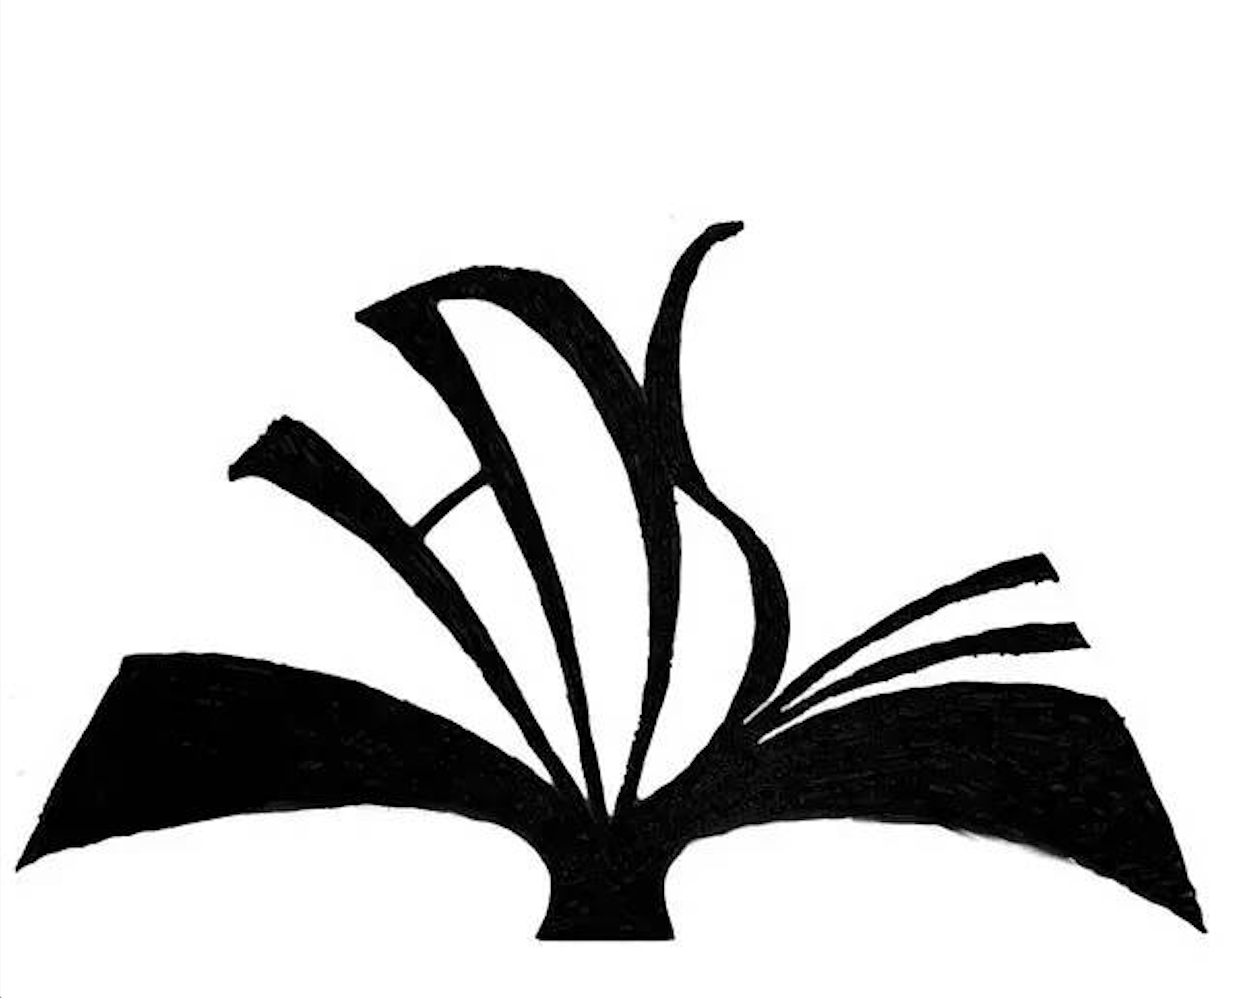
\includegraphics[totalheight = 0.5in]{logo.png}} %设置页眉logo页眉

% 页眉设置
\fancyhead{} % clear all fields 
\fancyfoot{} % clear all footer fields
\fancyhead[LO,RE]{\usebox{\headpic}}
\fancyhead[CH]{  \Large \kaishu 好读书} 
\fancyhead[LE,RO]{ \large \thepage}
\renewcommand{\headrulewidth}{0.4pt}
%\renewcommand{\footrulewidth}{0.4pt}

% ctexset
\ctexset{
chapter = {
    format = \raggedright,
    format += \Huge \kaishu \bfseries,
    pagestyle = empty,
    name = {},
    number = {}
},
%标题 楷体,加粗,二号,居中
section = {
    format = \centering,
    format +=  \bfseries \huge \kaishu 
},
%小标题(小四、加粗、楷体、居中)
subsection = {
    format = \centering,
    format += \bfseries \Large \kaishu
},
subsubsection = {
	format = \centering,
    format += \bfseries \large \kaishu
},
% 段落
% paragraph = {
%    format = \songti,
%    format += \normalsize
%},
space = auto,%如果空格后面是汉字,那么忽略,否则保留
punct = quanjiao,%标点符号为全角
}
% 章节出现在目录中而不显示编号
\renewcommand \thesection{}
\renewcommand \thechapter{}
% 姓名(小四、加粗、楷体、居中)
\newcommand \name[1]{\begin{center} \kaishu \Large \bfseries #1 \end{center}}
%\newcommand {\name}[1]{\kaishu{#1}}



% 页面设置
\geometry{left=2.5cm,right=2.5cm,top=2.5cm,bottom=2.5cm}
\setlength{\textwidth}{140mm}
\setlength{\textheight}{210mm}
\headheight 0.6in


% newcommand<命令>[<参数个数>][<首参数默认值>]{<具体定义>}
% newcommand 简单字符串替换
\newcommand\PRC[1]{People's Republic of \emph{#1}}
% newcommand 使用参数
% \newcommand\loves[2]{#1 喜欢 #2}
% newcommand 指定参数个数的时候同时指定了首个参数的默认值,那么这个命令的第一个参数成为可选参数
% \newcommand\loves[3][喜欢]{#2#1#3}

% renewcommand<命令>[<参数个数>][<首参数默认值>]{<具体定义>}

%\newenvironment{<环境名称>}[<参数个数>][<首参数默认值>]{<环境前定义>}{<环境后定义>}

\newenvironment{Quotation}[1]
{\newcommand\quotesource{#1}
    \begin{quotation}
    {\par\hfill ——《\textit{\quotesource}》}
    \end{quotation}
}
%封底

\newcommand \cover{
\raggedright

名誉顾问\qquad 贺美英\quad 白永毅

指导老师\qquad 贾 曦\quad  于 水\quad  池 净\quad 魏 晶\quad  顾彤彤
         
执行主编\qquad 谭明慧\quad 郎昆

责任编辑\qquad 王颖\quad 王书帆\quad 左婉\quad 孙泽华\quad 刘施扬\quad 陈俊新\quad 张凌波

封面设计\qquad 罗绮雪

出版发行\qquad 《好读书》编辑部

开\quad  本\qquad   210×140 1/32

印\quad  张\qquad   待定

字\quad  数\qquad  待定

版\quad  次\qquad   2017年4月第1版

印\quad  次\qquad   2017年4月第1次印刷

校内刊号\qquad TH-S-3006

印\quad  数\qquad   500册

}
%\renewenvironment{<环境名称>}[<参数个数>][<首参数默认值>]{<环境前定义>}{<环境后定义>}
\newcommand \undergraduate{

自动化系\qquad 颜钱明

精仪系\qquad 祝鹏飞

计算机系\qquad 姜伟峰

工业工程系\qquad 毛泽琪

社科学院\qquad 丁金萍\quad 靳天宇

化学系\qquad 梁家琦

电子系\qquad 余天呈\quad 张旭

热能系\qquad 邹逸宁

电机系\qquad 侯易岑\quad 杨欣淳

航院\qquad 陆俞朴\quad 袁李

经管学院\qquad 朱印\quad 胡惠怡\quad 罗汉\quad 刘康一\quad 王瑜

机械系\qquad 白怡杰\quad 王毅宣

软件学院\qquad 张育萌

土木系\qquad 樊双赫

交叉信息院\qquad 姚顺雨

法学院\qquad 李昱\quad 王志远\quad 王毅

新雅书院\qquad 张碧珊\quad 李怡恬

人文学院\qquad 屈晨钰\quad 姜宏志\quad 罗绮雪\quad 曾极麟\quad 廖青\quad 余娟\quad 李子平

生命学院\qquad 刘立荣\quad 吴妍

环境学院\qquad 王琦

汽车系\qquad 罗睿\quad 钱鹏

化工系\qquad 朱其盛

物理系\qquad 张世轩

数学系\qquad 黄臻

美术学院\qquad 刘德政\quad 高岑\quad 孙千雅\quad 徐洪斌

医学院\qquad 汪一凡

工物系\qquad 杨新宇\quad 周位鑫

水利系\qquad 嵇天颖

材料学院\qquad 梁宇晗

新闻学院\qquad 蒋茹茹\quad 陈芳婷\quad 高丽莹

建筑学院\qquad 杨晓霖\quad 薛靖凡

}

\newcommand \master{

自动化系\qquad 吕清

教育研究院\qquad 黄振中

精仪系\qquad 安迪

计算机系\qquad 王少清

新闻学院\qquad 张楚\quad 盛阳

化学系\qquad 邓耿

电子系\qquad 高玉荣

热能系\qquad 张琦

电机系\qquad 马子明

地学系\qquad 赖翔

机械工程系\qquad 于英飞

航院\qquad 白云祥

经管学院\qquad 尹西明

软件学院\qquad 刘瀚诚

汽车工程系\qquad 张晓前

水利系\qquad 王福山

交叉信息院\qquad 坑易澎

法学院\qquad 王玺

人文学院\qquad 修新羽

五道口金融学院\qquad 常华东

生命学院\qquad 汪伟

高研院\qquad 郑伟

深研院\qquad 魏乐业

马克思主义学院\qquad 付胜南

公管学院\qquad 凌争

微纳电子系\qquad 柏正奇

环境学院\qquad 何煦

化工系\qquad 蔡达理

物理系\qquad 邹昌炜\quad 陈佳斌

核研院\qquad 李明泽

美术学院\qquad 韦昊昱

工程物理系\qquad 赵骥

工业工程\qquad 王阳

医学院\qquad 黄镪

土木系\qquad 王庆

材料学院\qquad 冯一盟

社科学院\qquad 孙易

建筑学院\qquad 李紫薇

}
\begin{document}
\tableofcontents
%\name{我爱北京天安门}
%{\kaishu \raggedleft \Large 我爱北京天安门}
%\PRC{我爱北京天安门}
% \begin{Quotation}{易$\cdot$乾}
% 初九,潜龙勿用
% \end{Quotation}
% 字体族设置
%\rmfamily Roman Family or \textrm{}罗马字体
%\sffamily Sans Serif Family or \textsf{}无衬线字体
%\ttfamily Typewriter Family or \texttt{}打字机字体

% 字体系列设置(粗细,宽度)
%\mdseries{Medium Series} %\textmd{Medium Series}
%\bfseries{Boldface Series} %\textbf{Boldface Series}

% 字体形状(直立,斜体,伪斜体,小型大写)
%\upshape{Upright shape}%\textup{Upright shape}
%\itshape{}%\textit{Italic shape}
%\slshapl{}e%\textsl{Slanted shape}
%\scshape{}%\textsc{Small Caps shape}

% 中文字体
% {\songti{宋体}}
% {\heiti{黑体}}
% {\fangsong{仿宋}}
% {\kaishu{楷书}}
% \textbf{粗体}%中文的粗体用黑体表示
% \textit{斜体}%中文的斜体用楷书表示

% 字体大小
% \tiny{hello}
% \scriptsize{hello}
% \footnotesize{hello}
% \small{hello}
% \normalsize{hello}
% \large{hello}
% \Large{hello}
% \LARGE{hello}
% \huge{hello}
% \Huge{hello}
% \section{Introduction}

% 中文字号的设置

\chapter{清华读书人}
\newpage
\section{书香与流浪}
\name{曾小源}

我很高兴有这样一个机会,我们能够聚在一起,用自己的文字,谈谈经历,谈谈读书。
\subsection*{一 \quad 成长的书香}
既然是谈谈自己读书的经历和理解,我觉得就没有必要用太多学术性的话语,我的确也并无那种知识储备。对读书的理解,这真的是一个很大的话题。很多时候我们没办法给读书这个词下一个很准确的定义,它似乎是伴随着我们成长的一种自发行为。而我的读书经历,虽然大部分时间都与清华时光没有重叠,却无一不与清华有关。

为何?只因我在刚能记事的时候,我父亲告诉过我一句话——你的问题主要是读书不多而想得太多。

“这句话是谁说的?”

“清华的杨绛先生。”

不夸张的说,父亲在我那样年幼时告诉我的这句话让我第一次对清华有了初步的观感和向往,而读书习惯的养成,更是让我受益至今。也许唯有读书这件事,是我从乡野山村一直做到清华的,从后山、楼顶,到文图、北馆。似乎每读一本书,每经历一些事,每长一些年纪,对这句话的理解就会又多一分。

我已经记不得我读过的第一本书是什么了,不过我相信很少有人记得。小学二年级时,我偶然成为了《故事会》的忠实读者,每期都要买,每期都要看,连每月发行日期都记得清清楚楚,一个月两本,上半月八号出红版,下半月二十二号出绿版。我不知道为什么那个时候我会如此迷恋这本大众杂志,就像我也忘记了我什么时候开始对《故事会》感到厌倦,开始看《儿童文学》《少年文艺》,看曹文轩、王一梅、秦文君,也许是三年级下,也许是四年级。

五年级的时候,聚星天华出品的各种校园轻小说就像偶像剧一样在班上风靡起来,什么《天使街二十三号》、《麻雀要革命》、《泡沫之夏》、《会有天使替我爱你》等等,看了两本之后我发现我丝毫提不起兴趣,然后我迷上了网络小说。我想小学五年级到六年级这两年,我应该是把网络上有点名气的言情小说都看得差不多了,有些很出名的现在都拍成了电视剧,比如《后宫甄嬛传》、《步步惊心》、《美人心计》、《佳期如梦》、《来不及说我爱你》等等。

这之间也看过韩寒、郭敬明、张悦然、饶雪漫,也非主流过一段时间,看完了安妮宝贝的所有书,写了很多连自己都不清楚主旨的各种随笔,感觉就像是十一二岁的小男孩想写出自己四十岁的沧桑心态。但实际上我们都有这样一个“为赋新词强说愁”的年龄段,不经历这个过程,也没办法写出真正打动人心的东西。

然后,不知道从什么时候开始,也许是从初一的时候,我开始觉得我读的小说越发肤浅,总是一开头就能猜到结局,对书籍的选择也越来越挑剔了,在很长一段时间的书荒后,我开始看通俗文学,看中外名著,看钱钟书、王小波、陈忠实、契诃夫、茨威格等等,一直到现在。

回首我的阅读经历,就像是回顾我的成长历程。我很惊讶为什么有些家长要强迫孩子在三四年级的时候就去啃四大名著、唐诗宋词、诗经楚辞,那个时候我们连小学课本上的字都认不完能够有多懂得、多喜欢那些东西?如果真的看下来了,那也一定很痛苦,也许比我们现在去做考研英语的完型GRE的阅读还要痛苦。

我一直觉得阅读一定是要为了快乐,无论是知识的增长也好,字里行间的机智幽默也好,情节的扣人心弦也好,一定要让我们觉得快乐,觉得愿意读下去,如果觉得痛苦的话,真的没什么意思,我们没有到那样一个时间段,自然读不懂那个时间段的书。我们在每个年龄段读的书自然是不一样的,当然这个年龄段不是统一的。我觉得用这样一个词来形容这种过程最为贴切,就是“水到渠成”。

我觉得我做很多事情都遵循这样一个理念,细水长流,水到渠成,急不得。读书如此,学习也一样,很多东西都是融会贯通、相互联系的。就拿背单词来说,我有位高中同学高一开学就买了一本新东方的六级词汇,看起来无比高大上。我当然没有这个胆量。我是先背的高考核心词汇,然后背的考纲词汇,然后背拓展词汇,接着背了四级,最后涉猎了一下六级词汇。可能有些人觉得我这种方法好麻烦,但至少最后我的确完成了我的目标并且非常轻松,而那个同学高一开学买的那本六级词汇,我扫了一眼好像他还没有背完a开头的单词。我想原因一定是他看到满书的生单词就像小学生看到红楼梦一样,觉得痛苦,很悲哀,很绝望,觉得自己很渺小,很愚蠢,很孱弱,所以才不会成功,心急吃不了热豆腐。

我还想起了以前清华读书会推荐过一本书,叫《蒋勋说唐诗》,写得很好。蒋勋在里面写到,诗像是一粒珍珠,我觉得这个比喻很有意思。因为我们需要蚌壳慢慢地,慢慢地琢磨,最后才能得到一粒圆润无暇的珍珠,这需要时间,需要耐心。所以才很好解释为什么一到唐代,就像是历史的宿命一样,最好的诗,最好的诗人似乎都像是事先做了约定一样结伴而生。因为这之前有一段细水长流的准备期,魏晋南北朝漫长的三百年,就是琢磨“唐诗”这粒珍珠的过程,所以所有的惊心动魄,才方可珠圆玉润。你看,从阅读,学习功课,记忆单词,到一个人的成长甚至一个国家的兴盛文化进程的推动,都是细水长流水到渠成的一个过程。所以读书应该慢慢来,它会促使我们成长,也是我们成长的映照。

叶嘉莹先生去年在凤凰卫视华人盛典获奖时,我有幸在新清华学堂的现场聆其教诲。她说,写诗词或者文章要用心,这心在走路,那自然就写好了。其实读书的过程也便是读心的过程。说实话,高中以来我写过一些万能作文,每次只要小聪明似地改改段落,换一下开头结尾和标题,就马上改头换面,完美切合考场题目,然后无一例外地得分不低。我想一定有一些同学和我一样,并且对自己的机智颇为得意。但很多时候其实我很困惑,我们写了千遍万遍的李白苏轼,柳永陆游,陶渊明李清照,我们肆意引用故事里的风花雪月、风霜雪雨来为考场作文增分添彩,可我们真的了解他们吗?我们真的被他们感动过吗?也许我们自以为自己很懂得他们,但实际上,我们对此一无所知。

因为我们了解他们的目的时也许就是肤浅且功利性的。所以问我们关于古典诗词,我们也许知道很多,但我们从未亲身踏足于几千年前的长安城,秦淮河,几千年前的燕山雨雪,大漠风沙,我们宛如一张白纸的人生阅历如何足以体会里面真正的爱,真正的美,真正的欢乐,真正的悲哀。我们没有惊世才华,也没有被时代误解,更没有被时代抛弃,没有荣光万丈过,也没有独自出走,所以很难真正懂得李白“冠盖满京华,斯人独憔悴”的那种自负和孤独,前不见古人,后不见来者的自负和孤独,所以我们无法拥有李清照那种清高和超越时空的悲痛。

问我们关于信仰,我们也许知道很多。我们会联想到政治书上提过的民族区域自治制度,想到佛教道教基督教伊斯兰教,想到释迦摩尼老子耶稣真主安拉,想到十字军东征文艺复兴宗教改革,可是我们也许从未明白何为信仰,可我们也许从未到过藏地,看到那里天空湛蓝经幡摆动,看到蓬头垢面的藏民目光虔诚眼神坚定,对着苍天大地一步一叩,哪怕嘴唇干裂,膝盖流血,他们仍然要这样做。是什么支撑他们这样做?是信仰。所以我们可能不会懂得也不会拥有,因为我们怀疑一切,我们没有信仰。

如果问我们四大名著,我们也许知道很多,可我们也许并未经历过真正的繁华,真正的失去,我们没有经历过几十年的风雨飘摇,爱恨情仇,相聚别离,尘埃落定,所以如何真真正正体会到曹老 “满纸荒唐言,一把辛酸泪”、“败草枯杨曾为歌舞场”、白茫茫一片大地真干净”里的沉重和悲哀。只有我们真正地踏上那片土地,走过他们走过的路,呼吸他们呼吸过的空气,用眼观察用心感受,我们才会觉得我们到过的地方和看过的书形成了一种真正的相得益彰,在同一时间赋予了彼此更为深刻的意义和价值。因为有感同身受,才能够生出感动。这才是我对博览群书的理解。读书的过程,也是读心的历程,我们读书不仅要读得广,还要读得深。我们读的不仅仅是书,还是书里的那个世界,而我们看到的不仅仅是书里那个世界,还是书里的那个自己。也许那个自己很年轻,很青涩,他发现自己读得越多,知道得越少,没有关系,只要设身处地用心阅读,就能读到自己的成长,读到自己的心。

然而时至今日,这个园子的,或者说整个清北的功利心,是令我感到有些失望的。

高中课文也见,暑期学校也见,几番反复,才知道自己是不大情愿直面隔壁的蔡元培老先生的就职演说的 “入法科者,非为做官;入商科者,非为致富”“平时则放荡冶游,考试则熟读讲义,不问学问之有无,惟争分数之多寡;试验既终,书籍束之高阁,毫不过问,敷衍三四年,潦草塞责,文凭到手,即可借此活动于社会”。只觉每一句话都打脸生疼,不是我的脸,是好些人的脸,但总算是清北的脸。

我一直在想,蔡老所说的大学,和现在的大学,究竟是不是同一种东西。大学者,研究高深之学问也。现在的清北,又有多少人是认真读书、研究高深学问者,又有多少人成为了庞大社会机器各个角落的齿轮?清北仿佛已经不再是当年的清北。

这里有十数米高的建筑限制,雾霾太重时不见天日,人来人往,行走在瘆人的滤镜中。

社交,觥筹,活动或是玩乐,或是为了玩乐的活动,唱歌,跳舞,五颜六色的灯光,吵吵闹闹的音响,围桌而坐,不知聊些什么话题。而我总是那样一个人,在万人欢笑间独自沉默。

夜晚的冷风,吹醒了每晚颜色不同的夜空,吹散了多少梦。

终于明白,这毕竟是一个几万人的小社会,是一个不同观点碰撞的大熔炉,一个个体感受能够渺小到被乱流或群体呐喊淹没无声的清北乡。这里也不过是一群高智商,甚至只是成绩好的人的聚居地,不过是另一个小小的社会,不过是三千浊水中的一瓢均质。有人努力,有人堕落,有人看到希望,有人感到迷茫。一个蟹缸里,不过是另一个蟹缸,养着在同样均质中的涸辙之鲋。所以,别轻易谈起什么梦想。不是每个人都高举火把,更不会每个人都发光发亮。

钱理群老先生说,这里培养的是一群精致的利己主义者。实在是绝妙的说法,让人忍不住用“返璞归真”来形容。那些关乎人生的话题被遗忘,关乎未来的难题被回避,关乎信仰的问题被嘲笑,统统被这个浮躁社会中的浮躁小社会的碎片割裂,反射出有心人才能看见的冷光。

写到这里,抬眼看了看窗外。天已经黑了,被吹走雾霾的夜空之下,我看见清华园子的某些地方依然发着微光。我又想起杨绛先生那句话:

“你的问题是想得太多而书读得太少。”

于是我走进那钥匙形状的建筑物,站在一层的圆环正中心,旋转着,一圈又一圈。无数的书籍将我环绕,上通天文,下至地理,而我也许一辈子都读不了其中的万一。那时,我终于露出了一丝卑微,害怕错过了那么些人,那么些事,那么一段人生;怕自己配不上这国内顶尖学府,配不上那么多大神。

想到这些,我的眼里几乎是噙着泪的。

会错过么?
\subsection*{二 \quad 流浪生死}
\begin{center}
当秋天攀爬于藤蔓间

泪水滴落成蓝色的盐

亲爱的,在爱你之前,我一无所有

像危地马拉杜瑟河的河口

像矿山孤僻的手

像西藏的雪

像波兰的石头

我熟悉满布灰尘的房间

月亮所住的隧道

道别的严酷的飞机棚

荒漠一意孤行的风

……

——巴勃罗·聂鲁达

\end{center}
关于园子有多少值得回忆的事情呢,想起来竟然总是一些无关紧要的画面。

一天选修课的课间,老师让写一首自己喜欢的诗。我想起巴勃罗的诗集,却怎么也记不完整明晰,然后凭直觉拼凑一些印象中的句子,开始写字时发现,几个月没动笔,碳素墨水已然干涸。

一天下午一点开始的英语课,没有睡午觉的我瘫在桌子上,灯光,放映的幻灯片,模糊的人像,都成了虚幻不清的影子,嘴里竟然喃喃念到,山静似太古,日长如小年。

一个骑车的傍晚,看见操场上有熙熙攘攘的人在锻炼,看见街道旁接吻的情侣,看见飘落的两瓣梅花,地上的一个松果,擦肩而过的路人,零落的星子。走到五道口的十字路口,红灯有一分半钟,车辆经行的繁盛,如水流花开。那个宇宙中心的大世界仿似忽然变得很小,这一勺之地,却有沧海的水。

一天雾里的深夜,触目所及都是幻梦的景象,那天发了一条动态,说感觉自己像是走在澡堂里。被雾气感染的玻璃窗上,写下一串莫名的句子。

\begin{center}
你是哀伤弥漫眼前

雾气缭绕瞬间

词穷只剩画面

你是叶角细雪花边

日日夜夜晚安

秋水蒸煮细面

……

\end{center}

我希望周围的日子能繁忙起来,甚至希望有一丝危机和波澜,美丽的声色犬马,须臾的热闹喧哗,暗含漩涡,笙鼓齐作,我渴望这样的生活。我把所有水课都换成专业课,去了读书会,去了图书馆,开始拾起丢了很久的书。第一堂英语写作课,布置了一个作业,是写给未来自己的一封信。有同学问,为什么不能是写给过去自己的信呢?老师说,因为时光无法倒流,过去总是比当下慢半拍,而且只能被更遥远的事物已决定。你无法让过去的自己看到这封信,而未来的自己可以。那么未来,自己会怎样看这封信呢?就像时光胶囊,就像未名邮戳,就像蒙太奇。蒙太奇。这三个字让我想起之前那些为数不多的片段,就像把玩青苔,描摹残花,总是能唤起关于时间的回忆。然后时流如潮水,潮水逐烟尘,又总是不愿过多追思。在电影里,佳梅拿着玻璃瓶子当作话筒,黄昏显得落魄憔悴,风吹过乱发,弱不胜衣,她唱的是郑秀文的《娃娃看天下》。
\begin{center}

“脸上泛着微热

发上结着红蝴蝶

正是那段往事

我思忆中的七月”

\end{center}

七月。七月流火,八月未央。以前总以为是说七月燥热。某次做阅读摘抄,才弄明白“七月流火”是说大火星西行,天气转凉。一直认为这是一个很美的场景,如果在脑海里设想一下的话,有些经历,就像这个成语。小时候在茶店,夏夜总是澳热和溽湿,没有空调只有蒲扇,床单会被汗水润得汗涔涔的。此后很多年很多个夜晚,总是有意无意地回忆起这种单纯的潮湿,用回忆的力度仔细地摩挲复写之后,想起的却只有繁星满天,夜凉如水,就像激情褪去后的清冷与温柔。青春是一些相同情绪的代入,是模糊混乱的记忆,是散落的卡牌,定格在卡牌里的景色,又被重新拾起编写。比如铜梁安居的长街,比如磁器口的夏天,比如人民广场和中央公园,或者,在沙南街天桥旁三十五块一日的旅馆,窗内是摇摇欲坠的石灰和蛛网,窗外是破落的绿叶和灿烂急促的灯光,心思也这样破落而急促,无色的指甲油和无色的唇膏,涟漪一样的光芒,藏青色的天空,七月流火,八月未央。想起旁听的美学课上讲到,情感总是需要一些沉淀、间离和淡化,就像酿酒,在平静里回忆起来的冲动和悔恨,才有机会被真实地书写,就像如蝴蝶般颤动的七八月,往事不能被往事真实地记得。

在唇齿间缠绵缱绻多次的句子,何当共剪西窗烛,却话巴山夜雨时。可惜,这样的情境,却好久没在现实中重演。上中国文学史的老师在第一节课上感叹,他每周的课总是在周五,周五总让人想到离去,总是在下雨,下雨总让人觉得忧愁。有一种美的东西,人们接触到他的时候,往往会感到一种惆怅,陷入寂寞而无可奈何的境地。

老师说,人生五恨。一恨鲥鱼多骨。二恨金橘大酸。三恨莼菜性冷。四恨海棠无香。五恨曾巩不诗。

后来张爱玲改一恨,是红楼梦无续。

老师问,你有什么恨?

我有五恨。一恨水萍无根。二恨莲子有心。三恨微花易逝。四恨山海难平。五恨所念为君。

在自己的许多文章里提到自己初三时在冬夜里喝醉,下笔数行,情绪突破范式,当真以泪写成。那之后再没这样的体会,或是再没有醉酒的机会,也没有写文章的能力,愁绪难以排解,却逐渐找不到方式。黄山谷说,余不饮酒十五年,欲善其事而器不利,行笔处常常蹇蹶,总不如醉时所书。蹇蹶的原不是笔,束缚的是心,愁之一字,本就是心上之秋,哪怕啕号大哭一次,愁情并不能像泪水一样覆水难收,反之愈发汹涌。

看山是山。却总是不能懂得。

心生则种种法生,心灭则种种法灭。世间存在之法,生灭迁流,都无常住。为无常。

佛说,刹那永劫。

劫是一种浩大的时间概念。我们总是不知道在生命哪个片段,某个瞬间被无限复制,某个刹那能成为永恒。这些片段被长久地记忆,在生命的时空里产生扩大的意义,知无量劫只是一念,知一念为无量劫,当下恒远,刹那永劫。有一诗,记得绿罗裙,处处怜芳草。谁会在意草的绿色?可是对于这个人来说,心爱的人曾在春草尽头,罗裙浅绿,笑靥盈盈。这是一种很私人化的体验。一个人的记忆对于其他人来说,可能就是无足轻重,但对于自己来说,即是沧海天涯。

我时常会克制不住地想一位姑娘,连我自己都不知道怎么会有这些情绪,关于那些被定格和收摄的瞬间。老师讲王安石写《明妃曲》,意态由来画不成,当时枉杀毛延寿。他站在讲台上怔怔地问,你们生命中有没有见过这种美?真正的美是画不出来的。那一刻恍然,比如那天,春三月的某个公园,你在微笑,我突然有些发愣,然后时间固化成散碎的片段,像打碎的玻璃,像愁绪,像荧光,遇之匪深,及之愈希,无可描摹,只能存在于回忆中。

那真的很抱歉,我的双眼能看到整个世界,却只能在你的眸中看到我自己。而你的样子却在我印象里越来越模糊,可能再过不了几年,我会彻底忘记你的样子,只剩下一些微妙模糊的片段,比如袖口,比如睫毛,比如脸颊的雀斑,比如手的骨节,比如半透明的指甲。春镜即碎,破镜难圆,只剩下零星的玻璃渣子,予人徒劳拾撮。或许再过几年,我只能借助这些碎片的再现,别人看来毫无意义的物件,来印证你的存在,就像去年冬日看的那部电影,军车的前灯的亮光无意打在章子怡的耳垂上,那是晶亮璀璨的金黄色的樱花,会让日本人想到故国,想到脆弱易逝的惆怅。或者那天下午看的《爱乐之城》,广播里的钢琴曲响起,米娅突然泪流满面。所爱俱往,都是昨夜星光,胜过繁花无数,是无声念想。深情眷念凝结,流落于一个普通的耳坠,或是一首让人扫兴的钢琴曲。那将来我会怎样表达这种感情,以暴力,以深情,或以不能自已的哭泣?

佛说,梦幻泡影。

是夜,上完晚课,在紫荆公寓打着夜灯零零碎碎看完了《斯黛拉》,斯黛拉,她眼里的淡漠和成熟就像生长的枝蔓,年龄和身体却是晚开的花朵,深夜两三点,她坐在她深爱的金发老男人旁边,听着沉郁哀婉的音乐,看着彻夜狂欢经久不息的人群。那个人摸了摸她的头,让她去睡了。她的卧室通宵亮着灯,她能整夜听见楼下来往的行人,或亲吻,或谩骂,或打斗。她父母开了一家旅店,她和她父母一样,可能一生住在旅店里,混淆黑夜和白天的界限,含糊仓促又缓慢的时间,见惯游子浪人。

曾有人问,南开对于你来说是什么?南开对于我,就像这样一个旅店。说完这句话后冷场许久,再无后话。那时候想起自己半成年时的高一下,就像故事中的斯黛拉,困倦于那些焦躁不安的夏天,又不得安眠。南国阴柔萎弱的梅雨后,是蒸腾膨胀的湿气,还有四楼密闭的教室里,被中央空调冷却的关于夏季的热情。意兴阑珊的傍晚,电风扇转着,墨绿黑板上是向量的板书,课桌上是九块一杯的西瓜汁。无意间翻到那本黄色封面的教材,是王羲之的《兰亭集序》。是日也,天朗气清,惠风和畅。夫人之相与,俯仰一世。然后树叶簌簌零落,像在做梦,那一瞬间,想到一世。想到此地。我们都不可能永远呆在这里,只是或短暂或长期地寓居。这是旅店。我们,哪怕在死亡发生前,都不太知道自己是否在一个大梦之中,或以各地为逆旅,生生无所依。很多宗教或哲学流派都宣称,人有一个最终归宿,却不知道这个归宿在哪里,无归宿之前,即是在身体里客居,是在世界上做梦。做梦。寒暑假,或者在园子里的周末周日,常常无事可干,一梦就是一下午,是清明梦。在清明梦中,可以通过一些方法知道自己在做梦,比如捏住自己鼻子,发现自己还可以呼吸。既然是知道在做梦,总是想执意一响贪欢。在梦里可以执意去见想见的人而不必踌躇后果,可以上天入海体会失重的感觉,不必担心死,因为与梦对立的不是死,而是醒。而在普通梦境中,我们总是不能够知道自己做梦,所以即便梦中,也如有桎梏枷锁,做事常常夷犹,对失去无可奈何,正如人生某些片段,正如片段叠合的人生。这一刻突然想起庄周,想起李煜,想起苏轼,想起《红楼梦》,叹人生如梦的众位,或是真正在大梦中清醒,而不愿醒来。青春鹦鹉,杨柳楼台,如享太牢,如登春台,撕心裂肺的眷念,割舍不下的拘牵,难以磨灭的欲望,清醒者一响贪欢,因为醉生梦死,须臾之后,树倒猢狲散,食尽鸟投林。

佛说,流浪生死。

在塞北,在秦淮,在黄土高原的田垄上;在《百年孤独》的马孔多小镇,在《门口的野蛮人》里的KKR公司,在《忏悔录》里的圣皮埃尔岛…我在书页与现实间总是造次颠沛,流离失所,无枝可栖。伶俜于天地,环堵尽萧然。过于期待完美,却不能破烦恼之贼。人间世里,说到散木。散木也,以为舟则沉,以为棺椁则速腐,以为器则速毁,是不材之木,不可所用,能长寿。山木里,又说到雁,一只能鸣,一只不鸣,杀不鸣者。学生问庄子,山中之木,以不材终其天年,主人之雁,以不材死,先生将何处?庄子,在材与不材之间,似之而非也,故未免乎累。故未免乎累,就像庄周梦蝶。而自己也似乎也总是在两种极端之间,故总是觉得疲惫。内心是一个乱世,蛛为蝶之敌国,蜘蛛庸庸碌碌,蝴蝶翩翩起舞,故内心总是困兽犹斗,破碎支离,战事连绵,摇摆不定。
\begin{center}

如何是解脱之道?

佛说,谁缚你?

何处净土?

佛说,谁弄脏你?

如何是我自己?

佛说,骑驴找驴。

雪山喻大涅槃,心心如木石,什么是摩诃般若?

佛说。

雪落茫茫。
\end{center}

关于读书,关于清华,所有的经历与思考,大抵如此吧。也许与我同龄的太多人像我一样,总是感情太强烈太丰沛,而书看得太少。腹有诗书气自华,有理不在声高。我希望,身边的大家都能沉下心来爱上读书,做到真正意义上的博览群书,让园子书香弥漫的那一刻,便是配得上“大学”二字的那一刻。
\newpage

\section{灵性智慧$\cdot$读书}
\name{胡颖英}

下面我从世界观、人生观、价值观、读书四个角度梳理从书籍中获得的滋养。

\subsection*{世界观:关于“宜”}
天空下雨,伞儿撑起;雨滴入水,圈圈涟漪。我们是万千人群中小小的一员,行走在深深浅浅的路上。这幅巨大无比的画卷,有你有我,我装点了你,你塑造了我,无法分离。

三月的桃花像是春说的一句话,新绿的草叶喷薄着动人的气息,自由度极高的闲云,悠悠飘在蓝天上,原野上踱步的绵羊,闲散自在。我闭着眼听了片刻风的声音,细细的音乐,细细的喜悦……

经历着相同的晴雨,世界上的一切如此相宜,共存在同呼吸。

   “那阳光泄泄融融地铺开,桌、椅、窗棂,浴在澄明的光霭中,看上去像是静物图案。”是林徽因眼中的岁月静好;
   
   “请不要怀疑生命本身,在纯净的内心世界里,没有贫富之分,没有金钱的诱惑,更没有仇恨、贪欲的立足之地。以一颗质朴的心灵对抗一切世俗的侵扰。”是《小王子》童话里的世界;
   
   “微风在园中唤起一阵阵花浪,就像那静谧、柔弱的大海。浪花在绿叶丛中流逝,于是又现出花园和绿色的大海。”是米沃什倾听的《牧歌》;
   
   “一个孩子站着。他望着流水。远处:一匹马,背托一抹夕阳。”是哈瑞·马丁勾勒的《背景》;
   
   “吃豆花、看电视、为花草浇水、帮小猫搔痒……”是畿米优哉游哉的生活。
   
一切都峥嵘地存在着,却没有谁是一座孤岛。所有的宁静与纷乱,自由与禁锢,暴力与和平,黑暗与光明交织缠绕、更迭转换,有时相克,有时和解。有的只是常态,只是平衡,只是相宜。

\subsection*{世界观:关于“开”}

    牛根生:“凡系统,开放则生,封闭则死。人亦如此。” 
    
    鲁迅《呐喊》:“我虽然自有我的确信,然而说到希望,却是不能抹杀的,因为希望是在于将来,决不能以我之必无的证明,来折服了他之所谓可有。”
    
纪伯伦《哲思录》:“你们是道路,也是行路者。当你们中的一个人跌倒,他是为后面的人失足,使他们小心避开绊脚的石头。噢,他也是为了前面的人失足,因为他们步履虽然轻捷坚定,然而却没有挪开绊脚石。”
做一个心态开放、有逻辑思维能力的人很重要。我们总是先认识了身边的人,才认识了这个世界。封闭自己,不与外界沟通,会日渐狭隘;人家说什么就信什么,也挺傻的。认真阅读几本关于科学史和科学方法的书籍,很有必要。《把时间当作朋友》这本书不仅重点介绍了柳比歇夫“事件—时间日志”的记录方法,还给出了一些逻辑问题的处理建议,比如从多层面分析因果关系、进行辨析感悟(注意到“道理”和“感悟”之间的巨大差异)、交流守则等,强调专心提升自己,学习更多更好的技能,成为一个值得他人交往的人,并且独善其身,用自己的独立赢得尊重。

   《世界上最伟大的推销员》中有这样一个对话:
   
   “这里的人怎么样?”
   
   “你上一次经过的地方,那里的人怎么样?”
   
很大程度上,我们自己的处世方式决定了感知到的世界对我们的态度。不妨学习一下荷马·柯罗伊的方法。他并不年轻、英俊、富裕,也不假装久经世故,但每个见到荷马·柯罗伊的人很快就知道他是喜欢自己的。他让大家喜欢他的秘诀很简单:真诚地爱别人。问那个陌生人有关的一切:他来自什么地方?做什么事?有没有成家?他并非好管闲事,而是真正的对这位新识感兴趣,真心想知道这些。

\subsection*{人生观:关于“暖”}

   “兔子妈妈抱着我上山去看云,抱着我下山去看海。但山上的白云,山下的大海,我早都忘了,我只记得,兔子妈妈温暖柔软的怀抱…… ”——畿米《妈妈的怀抱》
   
快乐大概是上帝赐予我们最珍贵的礼物,快乐的笑容是活的,是灵动的,是颤抖着的,夫子“莞尔”,美人“嫣然”。只有真正快乐的自己,才能带给别人真正的快乐。

特蕾莎修女曾说:“我们做事的规模是否庞大并不重要,重要的是我们放了多少爱进去。”

快乐的服务生每天早晨总是连续3遍地问候:“早安!早安!早安!”态度诚恳;街上卖袜子的小伙儿热情地展示:“请您看看这些袜子有多美、多漂亮,真是好看极了!”脸上洋溢着庄严和神圣的喜悦,像是在向大家展示他所信奉的宗教的真理;小妹妹不小心摔了一跤,委屈得哭了,小哥哥竟在哭泣的妹妹身边故意也摔了一跤,同时一边看着妹妹一边笑个不停。这些平凡的小事,也是点点滴滴温暖的瞬间,因为有爱在散发光芒。

厄内斯特·海明威《老人与海》:“孩子走出了门,老头儿又睡着了。他依旧脸朝下睡着,孩子坐在一旁守护他。老头儿正梦见狮子。”

托尼·莫里森《宠儿》:“她把他给她的耳环包在衬裙里带走,不是为了要戴,而是为了留着。那对耳环使她相信,白人里也有好人。”

    川端康成《伊豆的舞女》:“舞女蹲在路边,用粉红的梳子替小狗梳理长毛。”
    
    陆幼青《生命的留言》:“雨,仍下个不停,但我分明感受到一种灿烂的金黄,向日葵般耀眼,莫非这正是陆幼青生命中最闪亮的颜色。”
    
这温暖的一幕幕,调亮了我们生活中温暖的底色。爱是一个正常心智的明媚选择,它积聚了一个人的精神能量和所有的素养智慧,是综合力量的体现。因为爱,我们有勇气面对困难和挑战;因为暖,我们不怕黑夜和冷雨的侵袭。正如奥格·曼狄诺所说,“没有一件值得一做的事情,可以在你的一生中完成,因此你需要希望。没有一样美丽的东西,可以在瞬间展现它的华彩,因此你需要信心。没有一件值得一做的事情,可以一个人完成,因此你需要爱。”每一天都是特别的日子,愿我们用心享受灵质的透明的美丽的快乐。

人生观:关于“守”

   “今早老太太起来的时候,其实老头已经醒来了。他从老伴的神情当中看出了她在想念死去的儿子,他有些不忍心丢下她撒手人寰。他心里想着:我要是撒手归天了,就只剩下可怜的她一个人了,那个时候,她一定不需要坐在那里煮咖啡了,想吃的东西还没有钱去买。今天又是个晴天,我一定要多割点草,中午的时候,我去把那片草地都割完。
   
    ……
    
他感到身体越来越支撑不住,但没多久,一捆牧草就归拢好了。他抬起头看看老太婆来了没有,好帮他扛在肩上,可她没有来。他试着一个人把一大捆牧草扛在肩上,但是牧草实在是太多了。他又试着背了一次,结果一下子摔在了地上。

……

老头子的脑海中还在幻想着明天去教堂、牧草如何长得更快、冬天该怎么过、儿子还没有尽孝道等事情。他望着天空,乌云在天上翻滚,仿佛死神铁青着脸看着他。

最后,他温柔地看了看妻子,慢慢地闭上了眼……”
                      ——节选自弗兰斯·埃米尔·西兰帕《暮年》
                      
作者的语言那么单纯、简练、客观,像泉水般清澈,反映出一个艺术家的慧眼所捕捉到的事物,从日常生活中创造出美,一份固执的守护,一种平淡的幸福。

    有人说,人生就像等公交车,有的人一会儿就等到了,而有的人却要等很久;有人说,只是期待就给了我内心无限的快乐;有人说,找一个喜欢的人、想回的家;有人说,世界上所有的美好,都有有效期限;有人说,若好事可以长久呢?
    
关于这个问题,我还没有想太明白。才刚体会到相信的重要性,我们要相信美好的事情会发生,或者即将发生,也只有当我们毋庸置疑地如此相信的时候,美好的事情才会当真发生。倘若必须选择相信好的事情会发生或者担心不好的事情会发生,何不选择相信美好呢。倘若觉得自己当下刚好遇见了幸福,那就尽最大努力去欢喜接受吧,不要再畏畏缩缩,再迟疑。一旦选择了,尽力去守护,凡是值得做的事情,都值得慢慢去做,做很久很久。

再分享两个故事:

作家E·J·哈地曾经写过,在纽西兰某处的墓地有一块陈旧的墓碑,上面刻着一个女人的名字和一些字:“她是多么温柔可爱。”这位哀伤的丈夫,把这些字刻在他妻子的墓碑上,想必一定拥有数不尽的幸福回忆。

作家三毛在《撒哈拉的故事》中描述丈夫荷西做完工回家时的情形:“六年了,回家时的他,怎么仍是一样跑着来的,不能慢慢地走吗?六年一瞬,结婚好似是昨天的事情,而两人已共过了多少悲欢岁月。”“不要去想五年后的情景,在我心里,荷西,你永远是活着的,一遍又一遍地跑着在回家,跑回家来看望你的妻。”

\subsection*{价值观:关于“格”}

    高尚的品格,具有非凡的魅力,是骨子里的高贵。
    
黄炎培写信勉励儿子:“和若春风,肃若秋霜;取向于钱,外圆内方。”这是谦逊、正直的品格;“若要优美的嘴唇,要讲亲切的话;若要可爱的眼睛,要看到别人的好处;若要苗条的身材,把你的食物分给饥饿的人;若要美丽的头发,让小孩子一天抚摩一次你的头发;若要优雅的姿态,走路要记住行人不止你一个。”这是奥黛丽·赫本的优雅;“科学本身就具有伟大的美。一位从事研究工作的科学家,不仅是一个技术人员,并且他是一个小孩,在大自然的景色中,好像迷醉于神话故事一般。”这是居里夫人对科学的痴迷。

做一个正直的人,干出漂亮的工作,活的充实精彩,有自己的理想和追求,还有一颗慈悲心,尽己之力帮助他人,大概是活出了自信的格调。

萨缪尔·贝克特《等待戈多》:“咱们走吧。咱们不能!干吗不能?咱们在等待戈多。”这是一份执着的等待;余秋雨《甘地遗言》:甘地墓碑上刻着“哦,罗摩!”,这是一颗崇尚和平的慈悲心;索尔仁尼琴《克列切托夫卡车站上发生的一件事》:历经几番交涉,佐托夫终于做到了让急缺补给的军车脱挂:“我只能为你做我职权范围以内的事,现在把你们脱挂,你们明天早上十点整出发吧……”这是超越忠于职守之外的体恤他人的善良。

这种心底的明媚,滋养出旷日持久的灵魂香气,指引着我们自立自强,努力做人,踏实做事,成为一个有责任、有担当的大写的人。“天行健,君子以自强不息;地势坤,君子以厚德载物。”作为年轻一代的科研工作者,投身研究,有所造诣,是我们肩负的历史使命,责无旁贷而无尚荣光。

\subsection*{价值观:关于“实”}

这里的实包括两个方面:感性层面的真实和理性层面能力的坚实。

    徐小斌在《羽蛇》中说:“无论多么精密的技术都永远代替不了‘感受’,那是一种亘古长存的真理。”人首先要忠于自己,忠于自己的心意。很多时候会为了别人难为了自己,跟自己说句辛苦。慢慢懂得,“度”字的分量。《传习录》曰:“人须有为己之心,方能克己;能克己,方能成己。”与自己的相处是一门大学问,自己是自己的知己、教练、最佳助手。塞菲里斯《茉莉花》:“不管是黄昏,还是初露曙色,茉莉花,总是白的。”无论遭遇什么,快乐也好,忧伤也罢,拯救自己的最终是也必然是自己本身,所以请善待自己,珍惜这一生的玩伴,一世的陪伴。
    
    理性层面能力的坚实主要指成长,或者说知识的学习与运用的一个实实在在的理由就是使得心灵能够成长。智慧与才华永远都是大受欢迎的,被需要是一种奢侈的幸福。
    
马尔科姆·格拉德威尔在《引爆点》一书中明确指出,引爆流行的三项法则:个别人物法则、附着力法则、环境威力法则,其中,一旦建议变得实际且符合个人需要,它就会令人难忘,任何观念要对人产生震撼作用,关键在于其内在质量。故要达成某个目标,非有志者不能成也,非有力者不能至也。自身能力的提高至关重要,且除了依靠自己勤奋之外别无他法。希望我们能够学而优则仕,不汲汲于富贵,亦可追求诗和远方。

\subsection*{读书:关于“灵性智慧”}

    “波提切利的《春》,描绘了这样轻灵幽美的一幕。春的女神抱着鲜花前行,轻盈的衣裙中散满着花朵。她后面,跟着花神与微风之神,更远处,三女神手牵手在跳舞,正中是一个高贵的女神维纳斯……至于三女神后面的那个人物,即是雄辩之神在采撷果实。天空还有一个爱神在散放几支爱箭。
    
草地上、树枝上、春神衣裾上、花神口唇上,到处是美丽的鲜花,整个世界布满着春的气象。”
                                    ——节选自傅雷《世界美术名作二十讲》
                                    
吴冠中先生的画作《长日无风》和徐悲鸿先生的画作《晨曲》有异曲同工之妙,交错的枝桠上栖息着三三两两的鸟儿,和谐而静谧,给人安宁的感受。

艺术创作是灵感的喷涌迸发,带给我们美的陶冶。

卡内蒂在《孔夫子做媒》一文中如此描述女管家对书的珍爱,基恩兑现允诺借书给女管家,他取了一本旧年装帧粗糙的书给她,她却把他的书放在一个天鹅绒绣花枕头上阅读,手上还戴着洁净的手套,她喃喃地说:“书永远是美的,人们应该理解到这一点。”

阅读是一件幸福的事,有时候读着别人的故事流着自己的眼泪,有时候觉得相见恨晚,书里描绘的可不就是自己的经历,顿悟我并不孤独,书籍就像纽带,让我们走进彼此的心里,娓娓道来的桩桩古事,呵护了我们的成长。读书是生活的一部分,感谢有书相伴。

书就像是可以飞到世界上任何角落的白色信燕,传递着跨越时空心灵相通的消息。

有幸与书结缘,故事未完待续……
\newpage

\section{我、书和三天}
\name{田佳丁}
\subsection*{第一天}
我的桌子上放着一本《流水四韵》。我坐在自己的凳子上,感觉有一丝的不爽。我是一个喜爱归类的人,而现在我却无法给这书找到一个让我完全满意的栖身之所。我试着回想这摞纸来到我的身边的原因,这一定是个莽撞的决定。我又在学校南门外的万圣书店漫无目的地闲逛。那是一个灰白色的雾霾笼罩的下午。几个小时前,我的签到课程因为老师有公务而调时间了,寂寞的梧桐叶还在冲着匆匆的路人招手。我已经在这熟悉的咖啡味中伫足良久了。在一排佛教经典和心理书籍的俯瞰下,一摊畅销书静静地躺着。

畅销书区的流动性很高,很多打着畅销书旗号进驻这一区域的书如果不能在登陆不久就给书商创造爆发式增长的收益的话,就会被请出去。当然也有部分书籍由于作者已经十分有名,或者有其他推广的需要,即使事实上无人问津,也可以在这里安然处之。推着嘎吱作响的手推车在店里转来转去的服务小生,把一摞一摞的书码放在柜上,就像厨师在上菜。畅销,就是诱使着这一列列张牙舞爪的作家们源源不断生产文字,并供养了一大批印刷厂和手捧着必备书单的文艺小清新以及商务人士的原动力。可经受住时间考验的畅销书往往是在它们跻身普通书架上的时候红起来的。

我在高中一年级的课堂上偷偷看从网上买来的整套刘慈欣的《三体》系列,书被物理老师冷不丁地从身后抽走了。下课铃声一响,他兴高采烈、如获至宝、大摇大摆地走向他的轿车,我竟然大胆地追出去了,我朝着他的背影有些焦急地问:“老师,书还能还给我吗?”老师打开驾驶座,冲我露出一个微笑,关上了车门,然后倒车起步而去。这书后来成了畅销书,在去年登上了“最受清华大学学生喜爱的书籍”榜单。同样是在高一的时候,我被《追风筝的人》橘黄色的霞光封面所吸引,如饥似渴地在贵阳的西西弗书店一口气看完之,还在看完后意犹未尽地买了下来。这书后来也成了畅销书。

我挨着把畅销书区里的生面孔翻了个遍,却没找见买书的欲望。我在书架的缝隙里转悠,不知什么时候,已经在回来的路上了,风呼啊呼啊地刮进我的领口,冷得我直发抖,我赶快锁上自行车,一口气跑上五楼,钻进了我的宿舍。

我凝视着一下午没上课的成果——一本素净的小说。在它的封面上,印刷的细的水纹由疏到密,由远及近,竖排的“流水四韵”每个字有一个笔画被拉长,指向四个独自的方向。下方还有竖排的四个字,“曹乃谦著”,底部是三联书店的广告语。朴素得有些派头的包装,这倒像是一本畅销书了。为什么我会在书店逛了一下午的历史和建筑书架后,买回这样一本书?我倒像是被这书背后的评语所蛊惑了——“像莫言一样,乃谦的天才好像是生来的。我读完《初小九题》的时候,恨不得马上把这优秀的著作译成瑞典文。”落款马悦然。这非常有外国人起名风格的名字,简短又侧面的评论,加上声称要翻译成瑞典文,虽然我对这个评论者一无所知,也并不熟悉莫言的作品,但这本书必定有些来路。

在浓郁的霾身后怠工了一天的太阳也要下班了,天色由白转为深黄,宿舍的楼道里也开始躁动起来。我现在毫无食欲,两只眼睛在书架上游弋着,想着将这本书塞到最好是一个不容易被看到的角落,如此,也许我就会很快忘掉这本有些另类的书,然后我就可以找几个伴儿,开始星期五的夜晚,直到某个阳光明媚的日子里来再次发现我的书架。

但我却想起了老师早上的话:“明天来加班呀。”这时,手已经下意识地撕开了透明的塑料封皮,细腻的纸页终于暴露在我的触觉下。一种莫名的期待让我打消了晚间娱乐的念头,催促着我快一些拿起这本书,最好在我的眼睛下班之前了解一下这书的看点。

于是我终于挣脱了我的凳子,抓着书转身走出寝室,推门进入了对面的隔壁的宿舍,然后绕过中厅,进入了也就是我的宿舍对面的宿舍,迅速占领了一把舒适的躺椅。我不在我自己的宿舍看这本书,一方面是因为对面房间有舒服的椅子可以让我躺下,另一方面是因为,我不喜欢我现在的舍友,他正疯狂地敲打着他的电脑游戏鼠标,拖鞋来回兴奋地搓动地板,噪声持续不断地刺激着我的神经。

我躺在祝鹏飞的椅子上,他的房间里飘溢着熟咖啡的味道,一台加湿器在吞云吐雾,窗外已经看不透天空,房间里一片漆黑。我打开夹在书架上的台灯。作者的第一章的标题是“进城”,我的眼睛快速地搜索着故事的人物。

“我妈是带着姨姨到大同看病去了,我已经有好长好长时间没有见到我妈了。我高兴得‘妈妈妈’地叫着,张开双臂迎着她跑过去。当我跑到了她跟前,她一下子把我给推向一旁。我没防住她会这样,后退了两步没站稳,冲后倒在地上,跌了个屁股蹲儿。我愣了一下后,正要张开嘴哭,可她却先哭开了。她不是哭,她是放声嚎,‘妈唉——妈唉——’。她就嚎就往院里走。我妈这么一嚎,我不敢哭了。”

我目不转睛地往下看。书的第一章就在说死人的事情,母亲带着姨姨进城去看病,姨姨却病死在城里,母亲用小平车把姨姨的尸体拖了回来,村里的亲人们都过来看了,姥姥、七妗妗,还有姨姨的女儿,七手八脚地开始料理丧事,办酒席。一些日子过去了,还没上小学的主人公“我”似乎已经忘掉这件事了,母亲突然决定要让“我”去大同县城念书,“我”只好跟着母亲上路。“我”和母亲起初坐大卡车,在路上颠簸了一整天,吸了一整天难闻的汽油烟味,车竟绝望地坏在距离大同县城二十多里的半路上,母亲和“我”只得走路,而母亲身上背着一百多斤的粮食,“我”只得自己走路,先是穿着磨脚的新鞋,后来干脆脱掉了鞋子,忍着痛光脚追着母亲的背影走了起来。

我用手撩了一下垂下的头发。这时书中的“我”已经双脚鲜血直流地跑到了大同,接着被母亲拉着前往小学报名。可是这时母亲却被告知,春季不招生,而且“我”的年龄还不到七岁,无法入学。母亲让“我”给教导主任背书,我背了“天地黄煌,宇宙黄黄,赵钱孙李。周吴郑王,寒来暑往,秋收冬藏……猪狗牛羊,沙果铜瓢。红枣黄梨,花生核桃。叉耙扫帚,锄头铁锹。豆角葫芦,萝卜山药……”逗得一个办公室的老师都笑起来了。然而学校还是不要“我”念书。就这样,“我”又返回了村里,直到八月份又回到大同,开始了初小的学习。

我不禁回忆起我的小学,那时我很能背诗,班主任语文老师让同学先在自己的座位上背熟练,背好了就到讲台上当着老师的面默写。我总是第一个上去的。而且一首新的诗只需要过目就能记住,所以往往我默写完了之后,过很长时间才会有第二个人到讲台上默写,不过老师似乎从来没有因为我背得快而表扬我。

书中的“我”则刚进入小学就接连受到了打击。先是班上有个叫“常吃肉”的同学要和我打架,而“我”记得母亲对我说过“到了学校甭跟同学打架”而不敢动手,后来“我”又被新班的班主任瞧不起,她骂“我”是“村猴”。晚上,母亲吹灭了煤油灯,“我”对于今后的学校生活越想越害怕,在床上哭了起来。

“嘿。”一只手朝我肩膀上拍过来,我惊得一下子坐直了,原来是看书看得太用力,鹏飞站在我的身边,看着我的脸说,“你在干啥?能让我一下吗?”我只好挪到另一个人的躺椅上。这个房间的四个人都买了可调后背的躺椅,不过“怀大师”最近去外地旅游了,近期不会回来。“天大”自从推上了经管学院的硕士,与女朋友在外租了一套房子,宿舍里包括自己的椅子都成为了仅用作放垃圾的场所。还有一个人“晖霸”非常邋遢,桌子上堆满了数学书、编代码的书、不知什么时候又买的水果,以及脏袜子。那水果总是吸引着远近周遭的果蝇围着它飞,我几乎没见过果蝇停下来过,它们就一直这样飞呀飞呀,也不觉得疲倦。我没有选择,只能就挪到去旅游的“怀大师”的位置上。

“你什么时候回来的?”我问道。

“我刚从实验室回来,今天老板一直待到十点半才走,学长学姐们都在那,我也不好离开,所以现在才回来。”他回答道,看起来很精神。我打诨道:“那你该不会是睡到了天黑才起床去的吧。”

“这怎么可能?老板看到我下午没去肯定又要说我呀。最近白天就在办公室里查资料、看文献,没完没了地。今天我找‘泷弟’借到了他的《银河帝国》,这个是讲科幻的,我觉得有意思就向他要过来了。”边说着,他掏出一本黑色封皮的书,直接打开了中间的某一页,凑到台灯的光线下开始了阅读。到了这时,楼道里一双双鞋的骚动声这时才传到我的脑子里,那些开完会、喝完酒、忙完作业和实验的男生们这时鱼贯而归,此时正是寝室的夜生活开始之际,往后的四个小时里楼道都将被这家的摔键盘声,那家的水龙头放水声,还有洗衣机的轰隆声填充。

自从高中那次被没收书之后,因为我的学习压力确实比较大,科幻书就没怎么看过,在大学里这几年,看着当年被没收的《三体》日渐走红,却不知怎么再也提不起重拾的兴趣,以至于看到鹏飞开始看一本翻译的外国科幻书,我竟一时也插不上嘴。我按开这张桌上的台灯,继续看起了手里捧着的《流水四韵》。

“‘‘我’一下子放开了哭声:‘妈,我想回姥姥家。’我妈说:‘咋了?’‘我’说:‘这里不好,我不想在这里,我想到大庙书房念书。’我妈坐起来,点着煤油灯。她看见‘我’满脸都是泪:‘孩子们欺负你了?’我说:‘嗯。’她问:‘那你不会告老师?’我抽泣着说:‘老师,也骂我,骂我村猴。’我妈说:‘好了。男子汉。不哭。’她一把把我按倒在枕头上,吹灭了灯。”

我搓捏着书页。我小学的时候,有个女生老是欺负我,不知她从哪里看的动画片还是电视剧,总喜欢学着那种城里人家庭剧的剧情,莫名其妙地冲到我面前,照着我的脸狠狠打一巴掌,然后跑开。我被打了好多天,竟然没有告老师,因为我从来不和别人打架,在此之前也从没有和其他同学打过架,甚至不知道这种事情是可以告诉老师的。后来有一次,我的脸被那个女生打得通红,回家后终于引起了妈妈的注意。她问出有个疯姑娘喜欢打我之后,去告诉了老师,老师在班上点了那个女生的名,也没惩罚她,不过此后那个女生再也不敢打我了,见到我都躲得远远的。这件事虽然妈妈其实没有出面,但我总觉得妈妈很了不起,那么霸道的疯女孩她都有办法治。小的时候,大家就是这样依赖母亲吧。

“第二天早自习课,张老师坐在讲桌前判作业。我妈领着我进了教室,她先跟‘我’说:‘俺娃回到你的座位去。’然后一转身,冲着张老师说:‘你跟我到校长那儿一趟。张老师直起身问:‘去校长那儿干啥?’我妈说:‘去校长那说说啥叫做村猴。’张老师嘴一张一张的,没发声。’我妈指着她,大声地喝问:‘说!什么叫村候?’说着,左手一把揪住张老师的领子……推着把张老师摁在了教室的门上……把她按得半蹲下……”

我正看得有些上劲,鹏飞突然转到我的身后,拍了我的肩膀,我回头看着他。

“周六去博物馆吗?我想去国博看个展览。”他说。

我想起明天要加班做实验、做设备,慢慢地摇摇头。

“走嘛,陪我去嘛,一天窝在宿舍这旮沓憋得慌,出门透透气也好让脑子清净一下,这样会帮助你思考更专注。”他说得一副很有道理的样子,台灯把他的眼镜照得白晃晃的。

此时我正看书看得进入状态呢,我回应:“我周末要在实验室加班,最近任务那么多,再不去实验室,老板就要上门来抓人了。”老板是我们学生对导师的称呼。

他看了看我的眼神,欲言又止,说:“好吧。”

我站起身,抖擞了几下肩膀,拿上我的书,走回了我的房间。室友正摇头晃脑地玩着他的卡牌类网游,念叨着:“来呀,来呀,你不是有伤害吗?我看你怎么办!” 头戴一副能将其与世隔绝的耳机。

我爬上了床,困乏得深深地陷入了被窝。我对这本无法归类的《流水四韵》正充满着新奇感,我觉得它像一缕紫烟,回香袅袅,我不想让它没有归宿地躺在桌子上,于是将它带上了我的床。我睁大了眼睛看着一行行字。

“张老师乖乖地站起来,稍停了一下,大声说:‘同学们,我说曹乃谦村猴不对。我错了。’我妈指着外面说:‘把这话到校长哪儿也说说去。’张老师两手合一起,连连地给我妈作揖,低声说:‘不能。不能。求您了,我,还没转正。我错了。求您了。’‘你还没转正?那好,爷爷放你一马。’我妈‘哼’地冷笑一声,转身走了。”

\subsection*{第二天}

我醒来时已经是八点了,今天是星期六,楼道里一片寂静。我的室友被先前那一拨早上约着出去玩儿的人在楼道里窜进窜出的躁动吵醒,现在正翻来覆去地试着入睡。长期熬夜玩电脑游戏的人在夜里往往很躁动,只能通过充分吸收早晨照射进宿舍的阳光来补充睡眠。我得赶紧穿衣洗漱,开始新一天的实验室加班劳作。昨晚被我放在床头的这本书,夜里一定睡得不踏实,我醒来后发现它躺在我的床脚,大概是被我睡觉时的翻来覆去给蹬到那里去的。

我将它放在了床下的桌面上,置于一堆辞典和工具书的上面。这些书虽然躺在我的书桌上,但因为长期不用,也蒙上了一层灰尘。

我做毕业设计的地方是一个被称为超净间的房间,在那里,为了避免实验器具受到空气中漂浮的粉尘或棉絮、头发等杂质的影响,每个进入的人都要把自己用专用的实验服从头到脚包裹起来,并在进入超净间之前经过一个密闭的隔间,吹淋衣物外附着的粉尘。在超净间内,不能使用手机或者自己带入的电脑等设备,甚至连未经清洁处理的笔记本和笔也不可以。整个区域被空气净化设备的轰鸣声所统治,宛如一个与世隔绝的太空城堡,四周被白色的塑料墙板包裹,黄色的乳胶地面上倒映着室内的每一处细节。

这是一个保密实验室,在第一次进入这里之前,我就要经过保密教育,其中最基本的就是不能与非该区域工作的人员讨论、说起任何涉及实现项目功能的具体的设备、设施或者结构。

我习惯开始干活之前先看时间,这样可以让我保持对我的效率的把握。房间内唯一能计时的工具是角落里的一台电脑,这台电脑是经过了无尘处理进入这里的,它控制着房间内的所有可以通过电脑控制的实验设备,平时我和这里的师兄、师姐和工程师们就通过看屏幕右下角来知晓时间。然而今天,这台电脑并没有开启。一位师兄告诉我,今天所有人都要进行零部件的加工,不需要用到电脑控制的设备,所以电脑也不开。

“别担心,到点会让你走的。”师兄告诉我。

我没有再问,转身投入了岗位。今天我给自己的任务是将一台设备的金属外壳加工好。外壳的毛坯已经委托工厂加工好了,我所要做的就是根据需要摆放连接的其他部件的尺寸和结构,在合适的位置上用电钻打孔、钻出螺纹,然后将细碎的零部件逐个安装、调试。在空气净化设备的轰鸣声中,整个过程显得十分地安静,只是我需要不停地抬起、翻转这个笨重的金属外壳,以找到合适的位置安装那些充满想象力且造型各异的自制零部件,就像翻动《海底两万里》中的机器一样。房间内有的工序需要暗光环境,因此在白天我也必须打着台灯,就像在看书一样凝视着我的作品。

我拿着一个零件在金属外壳上比划,嘴里念叨着:“我们做这种东西的时候就应该标准化,全部零件都做成一个系列的,固定连接的方式都成套,省得还要给每个零件单独测量、打洞、找螺丝。”

距离我的右手两米之外的师兄并没有反应,他正专心地用显微镜看着一些零件。我以为他应该与我有同样的感受,因为零件的尺寸、外观、表面位置各异,也给他的观察和检测带来了很多困扰,一些表面位置无法摆放在镜头下,或者镜头被阻挡而无法伸到聚焦的位置,另一些则无法很好地照明。

我又说:“这种装配的工作简直就是浪费时间,把零件做成一个样子就省时间多了。”

这不经意的话让我想起小的时候,妈妈总是喜欢说一句话:“思前想后。”她要求我把饺子包成一样大的,说这样储存的时候就不占地方,那时候家里用的冰箱是很小的,放东西必须提前规划。她要我先解冻大肉,等一会儿再拿出肉沫,先捡豆后切菜,这样就可以左右开工,节约时间。她连花盆都要求是一样大的,说这样子一个坏了可以把里面所有的花、土都挪到新一个里面,我说:“到时候再买不就行了嘛。”她连连摇头,说:“你就照我说的这么做罢。”

在这样的影响之下,我对事前的规划也形成了执念,喜欢把事情提前做完,喜欢提前将能想到的都准备好,有时甚至形成了某种强迫症。我买一样的矿泉水,一样的卫生纸,连是架上的书都是按照纸张的从大到小排列起来的。但是我又认为,这种排列必须要照顾书的种类,不能将内容不相关、以至于不能让我在阅读时产生相近的联想的书放在一起,因此,我在买书时又多了一套标准:书的尺寸。如果一本书的印刷开张太大或者太小,以至于和我已有的同类书无法放在一起时,一种无形的力量会让我放弃买下它。

这时我又想起了那本《流水四韵》,它现在应该还躺在我的桌上,在书架上没有它的归宿。

在我的左手两米外的工程师听到了我的抱怨,他对我说:“这些东西都是以前一代又一代的学生、工程师慢慢做出来的,原本也是从他们做完、用完、不用了的设备上拆下来的。每个人的设计思路、用途不一样,东西的结构尺寸什么的当然就不一样了。你现在是在捡漏,就只能将就了。”

我说:“那他们也应该考虑一下回收利用的可能性,总不可能自己不用了就扔掉吧。”

工程师笑了:“那就看你以后了,你做自己的系统的时候能不能想到别人想要用什么了。哈哈。”

时间过得很快,我继续埋头干活,时不时地给其他人搭把手,直到工程师伸了个懒腰,我知道上午的工作结束了——工程师是这个房间里最年长的人了,他的生物钟已经十分精准,当他感到疲倦时,就说明到了该午饭的点了。我的打孔任务还没有进行到一半,可我已经抱着这个沉重的铁玩意儿翻过来翻过去,累得气喘吁吁地,一点儿继续的力气都没有了。

中午饭是在离实验室不远的食堂解决的,一个南方人在北京待了四年,也习惯了馒头包子和稀饭,面条豆浆煮鸡蛋的饮食。当需要进行整天的脑力活动,比如数值计算、仿真、编程序时,中午就吃两个鸡蛋。现在是体力劳动时刻,所以我打了肉包子与稀饭,一开动就停不住,三下两下就把盘子刨了个干净。我回到宿舍换了身薄衣服,洗了洗脸。我的室友已经不在床上了,根据我的经验,这时他们大概会先吃饭,然后直接去自己进行毕业设计的地方,直到下午才回来。这时,我又看到了桌面上的《流水四韵》,这本书的封面白里泛黄,与深色的辞典一点儿也不搭。我爬上了床,中午的燥热让我睡不着,刚才在实验室中的困意神奇地一扫而光,取而代之的是窗外球场上的喧闹和电动车的报警声,还有风刮过树上枯叶的沙沙作响。

我迅速打开了书的下一章。书中的“我”需要完成学校布置的“积肥”任务,也就是去捡粪。“我”与那个霸道的“常吃肉”同学这时已经是好朋友了,由于城里的卫生改善,加上到处都在掀起“积肥”运动,马路上已经很难找到合适的动物粪便。此时,听“常吃肉”的介绍,“我”铤而走险地爬上了城墙,希望在一个常有人拉屎的地方找到需要的粪便,可最后却失望而归,因为这个地方的大粪全都被人铲走了。正在“我”为此感到无比懊恼,却又不敢告诉母亲自己需要积肥——因为母亲早就嘱咐过“我”,不允许上城墙,因为太危险,上了就要“打断我的狗腿”——的时候,母亲却带着学校开出的“大粪一筐”的收据回来,对我说:“学生不好好儿让学习,一天就让扫盲呀积肥呀。一满是不念书了。行了,这个礼拜你就好好儿在家学习吧。”“我”正感到诧异,问母亲在哪里找到了那么多的粪便,母亲说,是在城墙上。

这一章是我对这本书印象最深的一段,在这里,没有复杂的人物,在母亲出现之前,只有“我”和“我”的小伙伴两个人,童年的探险记忆就这样生动地回到了脑海,让我不禁失声笑出来。我想起了我在农村外婆家的童年,我在那里待到了三岁,那时可以在田间地头四处探险,可以和表哥们躲开大人的监视在清澈的小河边玩水,每次回到家被发现身上湿漉漉的,表哥们就要被狠狠训斥,而我却安然无恙。母亲在末尾带着“积肥”证明的出现着实出乎意料,而母亲自己去了不允许“我”去的“危险地点”捡粪,在这样的文字无声的冲击下的我几乎忘记了时间。

等到我往后翻了多页,却发现母亲在书里出现得越来越少,而“我”已经念到高小(那时的学制是初小、高小、初中、高中)时,时间不知不觉就过去了两个小时。我看了一下时间,急急忙忙将这本书夹在衬衣里,以最快的速度赶往实验室。整个下午我给这个笨重的铁壳打好螺孔又攻丝,然后将形形色色的零部件挨个儿装配上,然后还要将发挥功能的器件小心翼翼地固定在其上,连接各种线路,再将试验台清理干净,摆放上各种测量仪器,调整好位置。这一切的进行都十分安静,与身边的人配合默契到没有什么语言交流,时间也就过得异常地慢,干完这些已经是六点了。

本来昨天下午也应该像今日这样在超净间的隆隆声中忙碌的。昨天下午的课因为任课教师的原因暂停了一次,但我没有及时告知实验室的众人,他们以为我还在教室上着课,而我竟也捡了这个空闲,习惯性地去逛了书店。


我近来的晚饭也十分简单,一碗素菜,一碗面,几元钱就解决了。在这个季节里,乌鸦的喧嚣、食堂灶具和油烟机的轰鸣,都让我仿佛置身于实验室,催促着我以最快的速度完成我的“任务”。食物本该是人类最大的享受,历代文人大都不去写“吃”,因为怕俗,但只要写得好了像“停杯投箸不能食”,就能成为名句经典。可在我的生活里,吃饭真正地已经被淡化成为一个不起眼的片段,如果不是我的肠胃还保持着对饥饿的识别的话,我根本不会想起吃饭这件事。

我又进入了祝鹏飞的寝室,打开了一盏台灯,躺在了一张舒适的椅子上。这里依旧是一个人都没有,鹏飞去逛他的博物馆了还没回来,他的室友一个在旅游,另外两个在陪伴女朋友。而我的室友们现在正在我的房间里摇头晃脑地玩着电脑游戏。

我的阅读速度飞快,新的、旧的人物们在我的眼前群魔乱舞。书中的“我”寄居在大同县城里的五妗妗家,和院子里的邻居们成为了好朋友。母亲回到农村去种地了,因为她预感到国家的形势变化,知道三年自然灾害要来了,于是到农村去垦荒,给“我”在城里的生活屯粮去了。有一次母亲趁着半夜,坐着拖拉机回到城里,都没有进五妗妗家的门,等“我”赶出来,她已经返回了。“我”问五妗妗她来做啥,五妗妗把几盒苍蝇和几根耗子尾巴交给“我”,说这是母亲给我完成了“除四害”的任务,要我好好学习呢。又有一次,母亲趁着夜色坐拖拉机进城了,这一次,“我”半夜醒着,终于把母亲等到了,冲出五妗妗家去追母亲离开的拖拉机,终于看到了母亲被拖拉机的尾气和路上的风吹得灰头土脸的样子。后来“我”上了初中,再往后又上了高中,到了与哥们儿一起躲在校外喝酒的年纪,岁月里来往的人如织,作者行云流水的文字,不温不火,将一幅幅难忘的童年到青年的成长图景展开,濛濛似尘埃。母亲依然在那个村的那块地上耕种着庄稼,时而出现在城里“我”的身旁,给“我”送些好吃的,叮嘱我好好学习,否则要“打断我的狗腿”。

后来也不知是什么时候,我发现这间宿舍的唯一常住民祝鹏飞已经回来了。我问他今天做了什么,他说今天看了文献,拿了快递,打了篮球,在自己的实验室组会做了报告,和阔别多时的高中同学在五道口吃了东西,给自己的妈妈打了电话。我说这不同的实验室过的日子真实天差地别啊。他翘着嘴说:“这不就是个人的选择吗。选一个做商用产品的实验室,反正我也不会他们那些复杂的软件、算法,就水一水文献调研就好了呗。反正我已经推了经管的硕士,之后也不会再做这个行业了。”

他又开始和我畅聊他的《银河帝国》里的故事。那些剧情我也听得很是有趣,不过我知道那是科幻的瑰丽想象。在他的书架上,也摆满了书,虽然并不是书店畅销柜台上的那些,不过其内容都是讲金融、管理、现代名人传记、心理、成功一类的,另外,还有几本诗词书,也可堪支撑门面。鹏飞把这些各类的书无序地码放在书架上,有心情时就随意取阅,这大概也形成了他健谈的风格,想到哪里就说到哪里,轻松自在。

“现在是大四了,往昔一起玩耍的同学,如今连看见的机会都很少。我这个长期占着同学地盘的寄居生物,多了解一下朋友的意识家园,又有何妨呢?”我想。

\subsection*{第三天}

我早早地就醒来,虽然才七点,天已经亮了。今天又是一个大晴天,春风吹散了烟云,蓝色的天穹显得十分纯净,阳台外的梧桐上,枯叶在风中簌簌地作响。

今天是星期日,工程师们的休息日,我不用去实验室了。我起了床,发现我的《流水四韵》正躺在我的洗脸盆里。我连忙把书拿了起来,它只是沾湿了一个角,却并没有影响到里面的字迹。我的洗脸盆就放置在床下的地面上,脸帕则挂在床的一侧的挂钩上。“难道是昨晚看书太晚,忘了洗脸?”我几乎要这样说出来。

我的室友依然在熟睡,我收拾完卫生,小心翼翼地收起了几本书,背上书包溜出了寝室,来到逸夫图书馆的深处。反正这些人再过一会儿就会被楼道里其他人的唱歌声、关门声、洗衣机工作的声音惊醒,我可不想在他们醒来时被看到正在屋里,那样他们又要作出一副扭捏的样子,用晚上的疯狂敲键盘和晃凳子的声响来表达他们那“隐隐”的不满了。

书中的“我”有几个好朋友,“常吃肉”算资格最老的一个,他在小学刚开始时看“我”不顺眼,但在他的妹妹的干预下对“我”逐渐改变看法,我们成了死党,不过后来在学校组织的上山采集草药的活动中,因为“我”的建议,他的妹妹吃下了有毒的苍耳,死掉了,这件事儿“我”一直没有完全告诉“常吃肉”,我们的友谊得以维系。有一个叫“栓儿”的,是邻居狄大大家的儿子,一次在菜园里捡菜时与其他群体的小孩起冲突,栓儿为了保护“我”把另一个孩子打伤了,“我”由于钱不多,只能借给他二十块钱作为赔偿,他又为了凑剩下的赔偿去偷窃,结果被送进了少管所,后来时隔多年再次见到时,他还记得借了“我”的钱,并当面还给了我二十块,我推不掉,只好收下了。

我又想起了我小时候的玩伴们,王彬铸、唐冰、刘雪君这些人,大了之后也没了联系。我会和他们在院坝里爬树,有一次我贪玩了,本来应该去上书法兴趣班,自己不但没去,还给他们谎报“军情”,说是老师说了放假,结果下一次见到老师,我又对老师说是王彬铸告诉我不用来上学的,结果王彬铸被好好地“收拾”了一顿。不过这并没有影响到我们的友情,直到他转到其他的小学之前,我们都是好朋友。我在我家先前住的院坝里玩耍的邻居小孩,后来更是杳无音讯。是生活的轨迹将我们的童年岁月切割成晶莹的碎颗粒,每一颗都闪闪发光,每一颗都倒映出一轮完整的月亮,却无法被我完整地捧起珍藏,有一些就随着记忆的退却而消弭在泥土里。

在“文革”时,书中的“我”学习成绩优秀,自然要被塑造成代表,因为人缘也不错,就成了学校“文革小组”的成员。书中没有具体描写“我”在这一组织中做了什么,不过“我”却有机会经历了自己童年最崇敬也最亲爱的老师加朋友慈法师父被批斗折磨的过程。“我”在得知慈法师父被红卫兵找上门之后,跑回慈法师父家的院子住下,扶起了趴在地上奄奄一息的慈法师父,本想自己能做些什么保护他,却不想半夜里慈法师父上吊自杀了。这样沉痛的剧变让“我”的心灵有了巨大的转折,“我”自此失去了对“文革”的兴趣,逐渐淡出了学校的各种政治活动。五舅舅因为年轻时给国民党当过兵,这时也被审查,最后家人设法让他“压缩”到村里,才捡了一条命。而曾经打过抗日游击的母亲,对于种种乱象也不能做什么,只是尽力地出现在“我”的身边。在整个“文革”时期,母亲出现得比读书时候的次数频繁得多,这样的出现往往是带着“我”回乡下走亲戚、过年、吃酒宴,在那个“乱哄哄的”时候,这样的画风着实让“我”的世界温暖了不少。

我在图书馆的座位上一动不动地看完了整本书,太阳已经换了一边天空端坐了。

我站了起来,长长地伸了个懒腰,仿佛刚从时空穿梭旅行回来。我打开手机,想看看出去游玩的大家都有什么美图上传,却看到实验室的师兄更新了一条状态,说:“在实验室打电话给我妈抱怨工资待遇太低,竟然被老板听到了……”我一下子笑出了声。

我跑到图书馆外面,给妈妈打了个电话。我妈接了电话,先是问我吃了晚饭没,我当然照例无论吃了还是没吃都说吃过了。妈妈又开启了一连串的发问:“最近学习忙不忙?实验室有天天去吗?”我说天天都去,很累,她就说要注意休息,然后又问:“要和导师、师兄、师姐好好相处。”我满口答应。她又开始催我赶紧谈个女朋友,我也只能是不断地安慰她说现在正忙着,等到毕业了以后再说。

我妈说:“毕业了会不会更忙呀!你最好找个师姐带带你哇!我今天还在和医院的这些姨妈们说你,人家都打算给你介绍一个姑娘呀,这个妈妈看过的,又懂事又长得漂亮……”我连连推脱说:“哎呀妈呀,你别给我那么早操心了,我还要读书哇,以后会给你找的,我这种性质的方向以后也很难回家就业的,你可别老早给我规划这样规划那样的了,计划赶不上变化的。”我妈又放慢语速,跟我说:“那你就要好好加油,一定要留在国家需要的岗位,就在北京安家了,争取搞出点成就来。”我妈又开始跟我说家里的大事小务、姨妈舅舅们的动态,打完电话时天已经完全黑了。

不知什么时候开始,大概是从我高中离开家乡到省城读书之时起,我已经习惯了这样和我妈的长途通话。因为我妈不会用智能手机,她只习惯打电话,所以现在虽然有网络聊天工具,但我们还是坚持用电话的方式聊天。这样倒也省去了视频面对面时我回答她这些问题时的尴尬。

我妈妈是一名钢铁企业附属医院的医生,我小的时候她很少有时间带我,她最早教会我做的事情就是拿着钱去餐馆吃饭。那时候路边有一家餐馆,我在那里吃一顿肉菜只要五块钱,妈妈加班、值班回不来时,我就在餐馆吃饭,时间长了,妈妈和那里的老板也熟了。那个老板是女的,她的男人早前和她离婚了,她独自一人带着一个孩子,后来和在她家店里打工的一个男伙计好上了,剧情几乎就与后来有个叫《武林外传》的电视剧一样。后来,妈妈当上了科主任,加班、值班的时候终于减少了,可我却到了该读高中的年龄,妈妈仔细考虑后,还是决定让我到省城里的高中读书,自此我们家开始了三地分居的生活——我爸从我小学时起就开始在外地四处打工挣钱。

妈妈在我离开家的一段时间,先是尝试了去听流行音乐,然后又是学电脑,城里的孩子干什么她学什么。后来我考上清华大学、报了我现在这个专业后,她又开始关注国际新闻。现在我推上了直博生,她又开始关注军事动态,为了看一些军事、政治评论节目而雷打不动地守在电视机旁,堪比我见过的最狂热的韩剧女粉丝。这次与妈妈打电话,她又和我讨论了好些国防相关的话题,我说:“你这一天担心这个担心那个的,让我好担心哇,你应该多想想和平的事情。”我妈妈用她一贯的纠正语气对我说:“诶诶诶,你说的不对!你肯定要时时刻刻想着国家的发展、世界的局势,你们这种岗位上的人可一点也懈怠不得。”

每当这个时候,我就会感到选择了这个专业是多么幸运。

我还转过两扇门,看到了正在创作新的诗词的鹏飞。他对着窗外一片漆黑的夜色吟诵了一首新诗:
\begin{center}
问道精仪系,诗书对落霞。

远游三万里,看遍五洲花。

曾愿东篱看晴雨,今夕诗酒趁年华。

逝者如斯远,快哉共此风。

经纶谋宇内,入世化征鸿。

前路关山漫,此生风雨同。

归来对山月,百载一辈中。
\end{center}

我径直问他:“你今后的理想是什么?”

这样直白的问题可能不太诗意,回答不好就会很俗。他果然很俗地回答了我:“嗯。就是找个好工作,买个房子,生儿育女,孝敬父母呗。你突然问这个干嘛?吃错药了?”

我紧接着问:“那如果只能实现一部分怎么办?”他很配合地思忖了片刻,对我说:“那就先孝敬父母,生儿育女呗。”

我说:“我知道为什么咱俩儿合得来了。”

他用疑惑的眼神看看我,我注意到他的书桌上又入手了一本《基地》,科幻真也是写诗的灵感吗?

后来我跑了出去,在我的书架上为这本《流水四韵》腾出一截新的分区。细细数来,这又是我一个新的阅读习惯的起点。在我的书架上,第一层右边是我的实验室工作所需要的书,左边是我的科研笔记和读书笔记;第二层右边是历史类的书,包括各种史书、会要、通鉴、志疑,以及现代学者所写作的通俗史、杂谈,左边是语言和艺术类的书,既有学术类著作,也有书法、风水、语言词典和韵书;再往上,我有一些外国小说,它们虽然也多少可以算是与历史相关,但其视角和目标都与中国书籍有较大的区别,我不可能把它们放在一起。这样的书籍结构里,我没有为《流水四韵》这样的口述史、生活故事留出任何空间。我一直相信自己很强大,能够随心地驾驭我的人生,故而学习需要增长的就是知识和眼界。今天我却受到一点小小的打击,这书架也终于要承担起更多的意义。

我还给正在郁闷的师兄发去了一条微信消息,向与我同样工作在机器的轰鸣中的孩子推介起了一本书,我只告诉他,我的意念已经被强化了……

那一晚,我再一次看了书后的第二条评论,“流水四韵,三十六题,是作者沉淀一生的关于母亲的记忆。篇篇都在写‘我’,却又篇篇都在写‘母亲’。一位不识字的农妇的一生,本应是庞杂博大的一本书,但在曹乃谦笔下化为形式感十足的三十六则小品,篇篇都可独立阅读,却又相互勾连,最终显影出上世纪生活于中国北方农村的一位典型的母亲形象和其艰难波折的人生际遇。”署名王干。我又看了作者的后记。作者披露,自己是母亲捡来的孩子,母亲这辈子没有自己生育孩子,就带着“我”这个捡来的孩子,走过了风雨壮阔的一生,直到后来得了老年痴呆,再也不认识孩子了。

躺在夜幕里,我想,大学里读书的目的就是大学,在明明德,在止于至善。在信息的爆炸和碎片化同步进行的时代,珍贵的情绪往往是短促的,如被下岗、搬家、升学所割裂的童年记忆一样,唯有将这些细碎的簌簌声记住,通过自己的持之以恒的耕耘和磨练,才能演奏振聋发聩的人生乐章,这一路上,少不了生活的教导、感动、影响。三天与一本《流水四韵》,使我又想起妈妈忙碌的身影和我努力的过去,我要把书和这股澎湃的记忆,用生活的语言,传递给需要力量的同志们,让流水奏响凯旋的歌曲。
\newpage

\section{在阅读中醒来}
\name{岳廷}

唐诺在《查令十字街84号》的后记中写道:“人类发明了文字,懂得写成并印刷成书籍,我们便不再徒然无策地只受时间的摆弄宰制,我们甚至可以局部地、甚负意义地击败时间。”我一直以为,这是对阅读意义的最好阐释。

二十余年来,我从山村里对一切知识嗷嗷待哺的孩童,一步步走进了心中的知识圣殿清华园。这中间,无论迷茫失落、放浪张狂,始终有一页页的文字和书香在我左右,始终有古今中外的先哲智者陪伴身旁。我一度试图去解析阅读在成长时光里发生的化学反应,往往发现只是徒劳。或许,无论世界如何喧嚣,可以带着自己走进书的世界,然后再被缓缓合上的封底叫醒,如此周而复始,如此保持思考,就是读书对于我的意义吧。

说来惭愧,我的阅读启蒙从“偷书”开始。

一次轻描淡写的投资失败,让我的父母深陷一场与温饱有关的战斗十余年。这十年,是我的童年和少年时光。在那个不足百户的村庄里,我借不到书。而这个温饱线上挣扎的家庭,并不能拿出多余的钱给我买教材以外的任何书籍。我的哥哥大我七岁,那时已是一个挺拔骄傲的青年。他时常会带我到县城的新华书店看书。两个人充耳不闻售货员的责骂和驱赶,坐在冰凉的水泥地上如痴如醉得看一整天。但县城毕竟太远。

那时候,哥哥十分痛恨我们的乡村小学,最主要的原因便是小学的图书室只为迎接检查,从不对学生开放。于是在一个夜黑风高的当口,他做了一次精神财富的窃贼,从那间对我来说无比神秘的小屋子里盗窃了几十本书回来。因为这次盗窃,他度过了一段心惊胆战的时光。这些扉页上“图书馆资料”印记被哥哥用签名章遮盖掉的图书,有自然百科,有历史传记,有英雄故事,有童话传说。我一直认为,这一批来历不光彩的书籍,是我小学期间最隐秘而伟大的宝藏。

正是从这个巧合的机缘开始,阅读开始成为我这个寒门后生不可或缺的一部分。知识的丰富和灵魂的充盈是我在贫苦的求学时光中最引以为傲的资本。阅读,恰如一丝春天的细雨,寂静无声地滋润着原本干涸的心灵。

2013年我从清华毕业进入军队工作。初入行伍,一切都那么的不尽如人意:我找不到可以推心置腹的朋友,每天单调乏味的训练和公差让人实在找不到生活的乐趣。恰好在那个时候,我发现了一块宝地:连队的学习室。每天九点半,当确认所有战士已经有序就寝,我关掉楼道和洗漱间的灯光,一个人走进这间不大的屋子。那里有一个令人安心的书架,文学、历史、党建,麻雀虽小,五脏俱全。我会在这里平心静气地读一本书,或者只是发呆,或者胡乱地写一些零碎的文字。半年之后,我已经与所有战士打成一片,甚至有几个也爱上了阅读,每天在军号响过后,陪我一起来到这间学习室。那些零碎的文字也慢慢汇聚成河,有的发表在了杂志上,有的讲进剧本成故事,得到了广电总局电影局的扶持和认可。

就这样,阅读,永恒地与我的成长不可分割。

北岛说:“中文是我唯一的行李。”单此一句,就写尽了中文的分量和瑰丽。行李是一个容器,阅读让行李沉甸甸起来,写作则是一次对文字的重新发明和创造。这种内化和外化的互动和统一,是我用清华的四年时间学到的。

从大一开始,我成为了《清新时报》的一员;到大三时,我担任起这份学生媒体的文化版负责人。一年多的时间里,“文化”选题和写作的重压下,我开始大量地阅读有关清华历史文化的书籍。朱自清的《我所见的清华精神》,梁实秋的《清华八年》,三联书店的《清华历史讲堂三编》……正是这些书籍的阅读,让我更加了解了何谓“清华人”,让我有底气去书写今日清华人对这所学校的爱恋和思考。而这几年间的文字,也给我的清华时光留下了无数氤氲着历史气息的注脚。

2012年,适逢清新时报社十周年社庆,我有幸代表报社同仁,负责了十年清新人的作品整理和编纂工作。我给这本书取名叫《微观清华》。“微观”者,英文所谓“micro”,常态所不可见也,想了解最原汁原味的清华所不可或缺者也。这份以“清新”为名的报纸,在清华园的世纪沧桑中度过了自己的十岁生日,她的记者和编辑是清华园里一代又一代的本科生。21世纪最初的十年已经过去,大时代下的清华园里有多少大事小情正在悄悄地淡入历史的浓雾;所幸,这群孩子们用朴实的笔触、学生的视角记录历史、描摹人物、摄录春秋、评点时代,留下了这样一本迥异于清华宣传材料的真实体悟。

《微观清华》从那年暑假开始编纂,期间几次讨论和修改,最终于年底定稿交付清华大学出版社。奈何出版流程的限制,只能在十年社庆半年之后、101年校庆之时面世。半年时间里,全社同学齐动员,对书进行了多遍校对;这半年,学院的赵曙光老师先行帮我们印出一百本样书撑起了清新十年的庆典;这半年,我和同窗好友一起完成了三个版本的封面设计,最终有了成书的样子;这半年,我骑着一辆破自行车往返于编辑室和出版社,也算对出版的流程领悟了许多。在我毕业之际,这些回忆都被夹在了这本书的纸页之间,慢慢地飘散出无尽墨香,陪我走向天涯,行向海角。

就这样,《微观清华》,成为了我四年阅读和写作的总结,更是我走上工作岗位的“唯一的行李”。

对于我,热爱读书,如同岩浆崩裂一般不可遏制,是从本科毕业之后开始。正因如此,当我2015年回到清华园的时候,读书的热情相比起本科四年,更加汹涌澎湃。

我两年的工作中,很重要的一部分,是拍摄重大题材理论文献纪录片。特别大的选题,特别小的团队。初生牛犊不怕虎的精神,使我有胆量一个人挑起了一集的解说词撰写、拍摄文案写作、拍摄、采访和后期剪辑的工作。所有的领域都是全新的,千头万绪对于我都是挑战。

2014年夏天,我接到了拍摄澳门回归祖国15周年纪念纪录片的工作,分配给我的分集主题是“幸福”。策划阶段的全无头绪,我唯有再次选择到书中去寻找答案。一个月的时间,摆在我案头的,是杰弗里·冈恩的《澳门史》,是几大本的澳门经济年鉴,是各类关于澳门的文学作品。这些文字开始在我的脑海中拼凑出一个过去和现在都如此鲜活的澳门来。等到我踏上这片在脑海中由文字构建起来的土地,那些关于亚婆井的传说,那些市井小巷的百姓生活,开始与眼前的景象、采访的交谈慢慢契合起来。我想,这是每个读书人最想拥有的互文体会——恰如童年的我读完《猎人笔记》后开始无限地向往西伯利亚的猎人生活一样。

第二年,我的新任务是拍摄台湾的抗战史。于是,又是一次酣畅淋漓的阅读和探访体验。

回到清华园,我开始尝试一种新的读书方法:在每本书读完之后,只写自己感触最深的点,只写与自己思考切实有关的内容,完成一篇三百字左右的书评。如此一年多时间,我忽然觉得豁然开朗。我仿佛可以看见一本本书在我的生命中展开。他们形态各异,姿态万千,但都或多或少地与我的生命共鸣着,关照着我的过去、现在和未来。

去年冬天,我看完了齐邦媛的《巨流河》。我持久地回忆着我出生和长大的那个小村子,感慨旧时光与新生活之间二十年的沧海桑田,我在书评里写道:“逝去的时代和他人的故事,最大的意义当是展现一种生命的精神和风骨,当让你在书页翻动中回想起自己的人生。毕竟,幸或不幸,这都是我值得用信仰和爱去创造的时代啊!”

写罢,潸然泪下。

就这样,阅读以一种柔软的方式,持续不断地打磨着我的人生。

\newpage
\section{组诗之华园三幕}
\name{叶健文}
\subsection*{我所看到的凌晨两点的清华}
\begin{center}
路保留着灯光

情人保留着最后一个湿吻

从而把呼吸放慢双手抱紧\\
\ \\
寂寞深埋在紧闭的窗里

风隐藏着低温的秘密

横跨马路的猫大摇大摆

从来没有的得意忘形\\
\ \\
从学堂路的正南走向正北

带着点白天未燃尽的干劲,来——

一百二十度的扭头加六十度的转身

这个角度可以完美地诠释一次人生\\
\ \\
这里的夜是书页合上后被挤压的光

而总有在夹缝中无法入睡的人

担心明天来了,后天来了……

自己却依旧一尘不变

\end{center}
\subsection*{我所喝过的十年咖啡}
\begin{center}

我习惯了咖啡

温热,苦涩,和两片

从来多余的糖\\
\ \\
我喜欢独处

散文,诗歌,和耳边

不请自来的嘈杂

我热爱解剖

灵魂,肉体,和两性

复杂的同居关系\\
\ \\
我等待爱情

铅笔,毛笔,和钢笔

第一次划开的痕迹\\
\ \\
当然,我喝过

白的酒,真假

难辨,也抽过

卷的烟,焦油

尼古丁,记不得

什么样的味\\
\ \\
还当过演员,说谎

流泪,走心的自卑

做过盗贼\\
\ \\
童年,少年,青年

日积月累的罪

时刻都在忏悔\\
\ \\
但,最重要的是

我写过诗,长的

短的,尽是些

坍塌的文字
\end{center}

\subsection*{我在书中所未能遇见的}

\begin{center}

与你相隔

我孤身翻阅卷宗流淌的墨迹

暗黑的房间里不需要灯

以一个失明者的身份\\
\ \\
与你相隔

我始终跟随寺院的钟声

绕行青松千年遒劲的年轮

以一身杂念捆绑的俗人\\
\ \\
与您相隔

我努力穿越夜的半径直抵黎明

如同大海追念地平线上不灭的晨光

以一双残疾的腿日夜兼程\\
\ \\
与你相隔

岁月之两端,无法对折

我所深情发声的器官都失去功能

独白的悬念,只留给你一人\\
\ \\
与你相隔

方块字的演变史,至此至今

我吞咽过所有沸腾的文字,所以

平常的字句,并非没有深意

\end{center}

\newpage
\section{杂说$\cdot$读书在清华}
\name{潘子异}
\subsection*{一}
我以为,读书,重点不在书上。

写书的人儿千千万,初出茅庐的新写手、举世闻名的大文豪、之乎者也的诸子百家、怀才不遇的骚客文人、动荡一生的知青学者、标新立异的九零后。择书的人儿亦千千万,随眼缘儿的、奔着作者去的、旁人做媒的——自是千万种人,踩出千万条路。

书,虽有深浅,却是没有所谓好与不好的。正如要相亲的主儿,择书便是相亲,冷暖自知,媳妇儿哪有什么三六九等。合适的,便是好媳妇。读书之人自有择书之智,自择之人方有自读之趣。人生须臾,所读之书,自是沧海一粟;故所谓,读书,重点不在书上。

读书,重点也不在读上。

醉翁喜畅饮;读书人,你可爱酣畅淋漓,一气呵成?还是白酒太烈,只得小口抿,每日品上几页?你可爱唤来一碟花生米,做几笔摘抄?读书人,你爱去酒馆热闹;还是一人独酌,对饮三人?你的青眼,因陈年老酒而横?因新酿而横?还是洋酒?

读书人,你就是我,我便是你!怎样的读不是读,自是肠中千回百转,醉意朦胧!
\subsection*{二}
我以为,读书,重点是滋养,滋己养身。

这根茎渐见充实,它为一种崭新的感觉而动心;纤纤少女感觉到自己的乳房在圆胀起来时,亦是如此。——罗丹

不妨再加上一句:书读成了,亦是如此。

纵然在大白天,书中精髓完全被照亮,倘若不求助于心灵与思想,不在时间与生活的舞台上被自己全新演绎,则肉眼所能看到的,也不会比黑夜所见更多。也就是说,读书是一场自我修行与修炼。

“读后思,思后行”——这是一次修炼的全过程。限于经历与阅历,“思后行”确实不易;但“读后思”,是滋养自身的必然阶段。思想,冯虚凌空,以自我为基石,将书中精华,融以自我意识的浇铸,被吸收,从而达到新的眼界与心界——继而再择书,再读,再滋养。西天取经,九九八十一难,或易或难;一辈子的阅读,择书,或浅或深。打的妖怪多了,自然本领愈加地好;思的深了,自然修炼更深,择书的眼界也愈加地好。自我思想愈加成熟,自会尝些未试过的新的酒种,品更难懂的好酒,和那些本不起兴的苦涩的药酒;即使再尝浅酒,亦会品出新的意味来,而品酒的方式亦会愈加成熟。是所谓良性循环,也是“读书,重点不在‘读’与‘书’上”的根源:毕竟思的好了,“读”之法可自通;“书”之择可自选。

\subsection*{三}
    博尔赫斯说:“如果有天堂,应是图书馆的模样。”
    
    想来,自己是多么幸福啊!在最好的年代,遇到了最好的“天堂”。这是清华园的慷慨。
    
    这“天堂”里,你什么都可求。专业知识,人生感悟,脑洞,世界观,情绪,共鸣。这是著书人的慷慨。
    
    你可求,你渴求。如此才算不辜负这慷慨!
    
\subsection*{四}
    帕斯卡说:“人是一根能思想的芦苇”。
    
    那么,书,便是坻上的白色芦花呐。这些芦花,是一群大天使,展翅冲天,互相点头致意。它们日日便在这图书馆里,嬉戏玩耍,守着园里的学者与学子。

\subsection*{五}
\begin{center}

你说,什么会比那吟花的弱水

更涓涓长流?

是文字呐!

木挂绳结头,龟刻甲骨文

青鼎铸金文,丝织将墨留

一宣纸诉尽千万风流\\
\ \\
你说,什么会比那沉睡的青山

更亘古不枯?

唯有书啊!

子韦编三绝,生囊萤映雪

品诗词歌赋,藏四库全书

读书人尝尽五经四书
\end{center}

    如今,却是时代变了。手机呐,太容易便能牵来人的注目,咀嚼人的时间。它帮你把文字截成一屏屏的,帮你把时间切得碎碎的。只为留住你那转瞬即逝的注意力呐,它一遍遍地上演着“娱乐至死”的戏码。

于是这书啊,是一天比一天“难”读了。自省!

\subsection*{六}
有人戏说,那西游,不过是一场精心安排成自杀的谋杀。因为最终成佛为空。空即无,无即死。

读书何尝不是另一场西游呢?可这条取经之路,却是上帝精心安排的一场自救。你可以爬在作者的思想之上,拯救自己的无知引起的恐惧与茫然。读吧,思吧,自救吧!读书人!
\newpage
\chapter{水木书榜}
\newpage
\section{唯敢于想象者可与宇宙齐辉}
\name{梁乐萌}

多年之后,如果我已经把黑暗森林理论和面壁者计划都忘却了,《三体》唯一能够留在我脑海中的,或许只有这样一幅画面:

夜色沉暗,寂寥空旷的荒野中,只有一人安静地立着。在他的头顶,是广袤无垠的星空,群星大而鲜艳夺目,有梵高画作的浪漫风格。没有灯火,只有星星的光投在他的身上,拉出一道锋利的影子。这人仰头眺望着星空,没有望远镜也没有探测仪,他的目光却似乎穿越了生命本身难以跨越的时间空间,将宇宙尽头的奥秘投射在思想荡起的涟漪中。

读《三体》,感受到的是冷的光芒。因其笔墨纵横扫过太广的距离与太久的光阴,故给人以敬之寒畏之冷。可这种冷不是海沟最深处绝望的死寂,而是站在雪峰之巅,四下苍茫朔风砭骨之时,一道光束撕破天空从天而降,那是属于悲壮的勇敢者的光芒。

无论是《黑暗森林》最后超越人类理解范围的残酷宇宙生存理论,还是《死神永生》末尾宇宙告别田园时代,文明被二维化化作绚美至极的一张长卷,人类扮演的总是类似孤胆英雄的角色。宇宙的庞大与人类社会的渺小形成让人头晕目眩的对比,在这对比下,人类比被丢弃在茫茫沙漠中的婴孩更无助,无论面对宇宙真理本身还是高级文明的屠戮,人类完全无能为力。

可弱小至此,人类群体中仍迸发出几点细碎的光亮,在探索并维护文明的征途上留下了一笔华章。

《三体》中每个人有悲有喜,每个个体的故事都值得细细品味,但若将其中所有人物看作人类的整体,种种不同的特质与经历融为一体,却立刻展现出一种宏大的悲壮与美丽。

这悲与美,纵览整本书,又像是对现实中人类文明的隐喻。

《地球往事》的射手假设和农场主假设是这部书中众多光辉处之一,凡是追求真理的人看到此处大概都会心生寒意。“火鸡问题”最早由罗素提出,用来讽刺归纳主义者的荒谬可笑,可是刘慈欣拿来揭示人类对真理的探求程度并不能算是耸人听闻。

近代以来,人类的科学知识——无论是理论研究还是实际应用——都以千百倍于古代的速度发展飞跃,以至早在19世纪人们就认为已有的物理学知识已经是完备的真理,后人需要做的不过是数据的完善。可是,相对论如平地一声惊雷将沉醉于成就的人们炸起,量子力学、不完全定理,无不将人们原以为亘古不变的所谓真理推倒、撕裂。别怕,原来的理论不是错的,它们只是更广阔的真理的冰山一角。

以现在的视角来看,六百年前日心说是错误的,但是,它的意义并不仅仅是否认了“更错”的地心说。宇宙中心的改变,暗示着宇宙可能根本没有中心。同样,全新的科学理论做到的也并不只是对原有理论的推翻和扩展。当雄立几个世纪、简直被当作偶像崇拜的“真理”被质疑,人类被丢到了另一个恐慌之境:

宇宙间究竟有没有真理?

即便有,我们能否获得?

科学发展到今天,具有理性的人都应该认识到,不仅是皓首伏案倾其一生,就算用尽人类拥有的全部光阴,也不可能发现宇宙间的全部真理。一众科研工作者兀兀穷年,获得层出不穷的、令人眼花缭乱的新发现,也只不过像是比故事中还要渺小百倍的愚公,一次搬走一粒砂石,面前是望不到顶的巨峰。

人类的小,宇宙的大,对照来看总是让人绝望。人类不可能用脚步、也不可能用真理征服宇宙,可是人本身还具备着另一样强大的力量,强大到足以使人近乎造物的神明。

那就是想象力。

偏激的人认为想象是落后,是愚昧,是站在科学的对立面。那是痴人做梦,不是想象。想象不是顽固地扭过头不正视科学,一味沉浸在自己编织出的绚彩幻梦中,而是勇敢地挣脱旧思想模式的束缚,对事物给出自己合情合理的富有创造性的理解与判断。

想象不仅不与科学相抵触,还常常帮助科学发现打开新的天地。如果没有超凡的想象力,达尔文会安然接受统治几个世纪的万物神创,孟德尔不会把目光移向田野里的各类豌豆,薛定谔又怎敢对物质存在形式提出质疑?科学是想象落地后的延伸,想象很多时候可以为科学开路。

想象的意义不止于此,它赋予人的还有哲学意味上的高贵。

古代中国有天圆地方之说,“天之包地,犹壳之裹黄”。古印度人认为乌龟蹲在蛇身上,支撑大地的象群站在乌龟背上,太阳在上方旋转。现在的我们觉得这些说法荒诞不经,甚至斥之为愚昧无知,可是我们现有的知识,在宇宙真理的视角来看,或许只是五十步笑百步。

人是渺小而脆弱的,可他的伟大之处在于有心、有意识,也就有了对宇宙万物的想象。他目光所及只是宇宙空间尺度中的一隅,却能在想象中飞跃无尽的距离。他存在的日子只是宇宙时间尺度中的一瞬,却能在想象中游历无穷的光阴。

这正是老庄的伟大之处。如果说儒家心有天下,道家则是心有宇宙。老子说,“道生一,一生二,二生三,三生万物,万物负阴而抱阳,冲气以为和。”庄子说,“野马也,尘埃也,生物之以息相吹也。天之苍苍,其正色邪?其远而无所至极邪?”时代局限了他们对狭义科学的探求,却没能禁锢住他们对天地万物恣意汪洋的想象。他们冲破了天命观,不再将一切挂靠在一个高度人格化的狭窄的“天”上,而是想象出了“道”这一玄妙至极、广远至极的概念。他们说道创造了万事万物,人类的想象却创造了道。

这也正是《三体》以及其他科幻文学的伟大之处。我们不应该苛求科幻文学中的想象就是绝对的真理,更不应该苛求它们在日后被科学发现所证实,毕竟科幻文学不是科普读物。从开山之作《弗兰肯斯坦》,到诡异怪诞的《最早登上月球的人》,再到刘慈欣的《三体》、郝景芳的《北京折叠》,科幻文学作家的可贵之处在于,他们作为人类群体中的一员,勇敢地用想象挑战宇宙的广漠与神秘,引着人们暂时从生活琐事中抽身,将思想投向只有思想能到达的地方,并使人们在那些存在于另一个时空的人物身上得以窥见自身的影子。

2017年2月末,美国国家航空航天局(NASA)宣布,在距离地球近四十光年的地方发现了七个大小与地球相仿的行星,并公布了一组“高清大图”。在图像中,七颗行星有的被灰白的岩石包裹,有的泛着微绿的柔光,有的上空蒸腾着斑驳繁复的云雾,新奇,却又亲切。

然而,这些图像其实只是天文学家和艺术家在已知数据基础上合作的艺术品。NASA手中真正拿到的,只有探测器传回的断断续续的电波。

可是,面对这些美的让人屏住呼吸的图像,谁能责怪天文学家胡思乱想?谁能不被这些永远不能亲身到达的星球的美所震撼并浮想联翩,反而坚持认为想象有违科学的严谨?有这样一群人,他们不因获得数据之少而绝望,不因永远无法看到星星的真实面貌而消沉,还能以乐观幽默的态度用想象力为星星画像,这正是可与宇宙比肩的伟大勇气与胸怀。

因为有想象,人才可以在一拳之大的心中放下整个宇宙,张开双臂便是六合八荒。也正是因为敢于想象,人们才不会在宇宙面前像个柔弱的孩童一般抱紧身体畏缩不前,而是勇敢地将自己微小的生命掷入宇宙之中,一次次去验证自己的想象,一次次用想象对宇宙作可歌可叹的征服。

宇宙之伟大在于包罗万物。如果人能以想象在心中创造万物,虽然渺小,也就不比宇宙逊色。

从前读书时觉得万户愚蠢。可现在我说,没有万户心中乘火药风筝之力升空的想象,就没有今日飞机凌驾白云之上的飞翔。

\newpage
\section{男人,女人,执剑人\\——解读《三体》中的人物:罗辑}
\name{朱大有}

面对强大的三体世界和未知宇宙中潜在的威胁,人类命运的转折点,是后来被评价为“幼稚”的面壁计划和“面壁者”罗辑。作为人类文明中的独特人物,也作为《三体》承上启下的第二部《黑暗森林》的核心人物,罗辑这个角色串联起了许多个性各异、却恰恰因此组成了人类这一群体的人物。逐个分析、对照这些人物之后,我们也得以全面地把握、解读罗辑。以下便以这样的方式行文,虽以其他人物作为小标题,但全文意在展现罗辑这一人物,可谓罗辑的人物志。

\subsection*{跳出人类局限的第一人:叶文洁}

在第二部开头,叶文洁教给罗辑宇宙社会学的两条基本法则,为之后罗辑的黑暗森林理论奠基。如果不是叶文洁选择了罗辑,人类就无法从地球背叛者与智子通信的记录中获得罗辑这个名字,罗辑也就不可能成为面壁者。值得推敲的是叶文洁为什么选择了罗辑。除去罗辑是叶文洁女儿杨冬的同学的巧合,叶文洁应当还有其它考虑因素。

经历了文革磨难又独自在红岸基地秘密与外星球交流,叶文洁的心智已非比常人。她亲手杀死丈夫,并不是出于仇恨等属于人类情绪的因素,而毋宁说是超出人类之外的某种意义——叶文洁坚信三体世界的发现对整个人类有更高层级的意义。人类的局限性就在于爱,这一点在《三体》的后文中多次印证。叶文洁是跳出这一局限的第一人,在杀死丈夫的那一刻她就已超越爱情与亲情。讽刺的是,杀死丈夫之后,叶文洁经历了她人生中最温情的时光,产下女儿杨冬后住在村民家中,受到村民无微不至的照顾,俗世的生活使她再度找回人类世界的美好。但那时的叶文洁已然回不去了,刘慈欣写道“在叶文洁的记忆中,这段日子不像是属于自己的,仿佛是某片从别的人生中飘落的片断,像一片羽毛般飞入自己的生活。”既已超越人类的喜怒哀乐,这样的生活就再不可能真正属于她。

罗辑具有类似特征。罗辑缺乏作为一个普通人的爱,起初在爱情和事业上他都采取玩世不恭、得过且过的态度,很难看到他有因为热爱而生发的热情。倒是他因幻想而生的爱情,很有几分超越俗世人类的特质。在刘慈欣的描写中,无论是作为地球三体组织领袖的叶文洁,还是作为执剑者的罗辑和程心,事实上都不再被视作普通人类,而具有近似“神”的地位。

成为一名执剑者,最紧要的素质是威慑度(根据第三部的内容,只有三体世界有评测威慑度的技术,地球世界没有,否则不会选择威慑度只有10\% 上下的程心)。威慑度说白了就是毁灭地球的决心,因为毁灭作为敌人的三体世界并不需要下什么决心。对于一个拯救地球的人来说,最大的障碍就是地球本身,谁越能下决心毁灭地球,谁的威慑度就越高,就越能拯救地球。这正是程心的困境,她从来没有下毁灭地球的决心,“她在潜意识中不相信现在的事情会发生(第三部,第136页)”。这是一场和三体人的赌博,地球人手里的筹码太少。

因为筹码少,所以就要像维德说的一样“不择手段”。执剑者不但不能有爱,甚至不能有最基本的道德,他必须拥有一颗随时承受毁灭一个文明的压力的心。人类的对手文明程度比人类高太多,要拯救人类,就要超越人类。在超越杀戮与道德这一点上,没有一位“面壁者”例外,叶文洁是开始,维德是结束。

\subsection*{大史:生存即谦虚}

大史是《三体》中罗辑唯一的知己,尽管相对于叶文洁、罗辑和程心,大史只是个普通得不能再普通的人,但他却是唯一理解了罗辑的人。他曾对罗辑说,他和罗辑是一类人(第二部某处)。

二人共同之处是谦虚。大史虽然粗犷,却总能知道自己能做到什么,应该做什么,然后好好去做,而从不逾越自己的权限范围。儿子犯了罪,他说的是帮不了儿子,儿子得自己承担责任。尽管拥有职权,大史始终把自己当作普通人看待,在地球舰队被水滴毁灭后的混乱中,大史被任命官职时表现出的诚惶诚恐之态便是印证。

其实罗辑同样想做一个普通人,这是刘慈欣描写的罗辑这个人物的矛盾之处。他玩世不恭的态度有出离普通人的趋向,然而他又始终安于现状并不奢求,愿意混混日子做一个“俗人”。在获得面壁者的权力之后,他的第一反应是承认自己不可能拯救地球。在利用面壁者的权力找到庄颜在雪山下定居后,他再不动用权力调动任何资源,安于个人美好的生活。要不是行星防御理事会逼迫他,他一定想不起还有两条宇宙社会学定理。

大史因谦虚而谨慎,这一点使他救了许多人的命,包括罗辑。四位面壁者中,泰勒、雷迪亚兹和希恩斯看起来都比罗辑合格,然而谦虚的罗辑才是救世主,前三人制造的希望被证明只是泡影,而罗辑发出的看起来像泡影的广播信号才是最终拯救人类的钥匙。刘慈欣在《三体》中反复强调,人类要想在黑暗森林般的宇宙中生存,就必须保持谦虚,大史和罗辑无疑是这样的“人类”代表。

\subsection*{雷迪亚兹:英雄死于道德}
面壁者的计划中,雷迪亚兹的计划其实和罗辑的计划最为相像,都是制造对三体世界的威慑,唯一且关键的区别在于,雷迪亚兹的计划实现难度大,威慑发生时间长,使三体人有很大的阻止可能性,所以无法像罗辑的计划一样把地球和三体世界拉到同等的地位上对话。

因此雷迪亚兹的结局也就比罗辑悲惨很多。罗辑面壁五十年得来“不感谢”,而雷迪亚兹满含深情地呼唤本国人民,换来的是压死他的漫天石块。对于这两个为人类生存付出部分或全部生命的人,人类并不视为英雄,反倒像是仇人。因为二人都有可能毁灭全人类的生存,就不可免地受到谴责。这种谴责忽视了二人的前提都是为了人类生存,而只顾及道德上的意义。扔雷迪亚兹最后一块石头的老太太说,“恶人,你要杀所有的人,那里面可是有我的孙子,你竟想杀我的孙子!(第二部,第274页)”,对这位老太太来说,全人类的生存未必比其孙子更重要,道德高于生存,或者说,个体往往无法超越于自身的道德伦理,而站在人类的整体立场上承担生存的重任。

然而要在宇宙中生存,生存就要高于道德,但当生存危机不那么迫近的时候,人类往往容易忽略生存的重要性。如果人类没能生存下来,青铜时代号也不会遭到审判,而结果相反,人类生存后捡起道德,用道德杀死了青铜时代号。三体世界不允许爱,歌者世界甚至不允许精神自由,在生存面前,道德和爱一起变成了人类的局限性。

\subsection*{程心与维德:相信人类?}

罗辑为什么把“剑”交给程心是令我疑惑的。尽管人类无法评测威慑度,但罗辑是第一个执剑者,五十年威慑岁月不仅洗白了他的头发和胡须,同样也必定使他的精神和眼光达到了人类从未有过的高度。罗辑很有可能看出程心的威慑度远低于自己,是一个和自己很不同的人。那么罗辑为什么愿意拱手把全人类的命运交给一个不合格的执剑者?

可能的解释有:一,政府和行星防御理事会的压力,这个不太讲得通,因为罗辑一贯不太在乎此二者,他选择成为执剑者也很难说是慑于它们的压力,何况它们还用庄颜作为手段逼迫他工作;二,在漫长的岁月中自己已经疲累,同样讲不通,后文可看到罗辑过百岁仍然精神矍铄,而且既然他选择成为执剑者,必然不会以此为由逃避责任。

唯一的解释是他选择相信程心,在程心的身上,他看到了极低的威慑度,也看到了与他相同的人性与爱。他当然可以根据自己的判断,提出为了全人类的生存,程心不适合成为执剑者,然后握起剑柄威慑地球。可这没有意义,如果人类必须永远庇护在他的身后,就会是永远长不大的孩子。如果他威慑地球,维持自己的执剑者地位,地球会再度陷入恐慌,他会成为和三体人一般无二的对地球的威胁。这时的罗辑扮演的是人类父亲的角色(第三部的罗辑的角色已变得平面化和脸谱化,但在最后太阳系二维化的过程中罗辑和程心的关系明显很像是父亲和女儿),他愿意再赌一把,看看人类依靠自己的选择,而不是外在的“威慑力量”支撑,是否能在宇宙中生存下去。

维德的选择其实同样如此。维德是个守规矩的人吗?这是个可笑的问题。情况类似的是,此时的维德也已是一位老人,他对地球目前形势的判断很可能比程心精准,他自己也知道这一点。他可以违背诺言,拿起反物质武器为人类的自由而战,那将成为他最后而永恒的辉煌,只要他愿意。但他选择了相信程心,注意程心是一直年轻的——在这一连串的危机与变革中,人类时常流露出幼稚的地方,也始终有足够成熟的人站出来,但只有他们是不够的,人类幼稚的一大来源是因为有爱,是因为做不到“把自己的妈妈卖到妓院(维德语)”,那么,即使这些足够成熟的人以限制甚至扼杀人类的爱的非常的手段暂时延续了人类的生存,如果人类自己不变得成熟,也没有意义。

换言之,既然人类作为一个物种和文明选择了拥有爱,而不是像三体世界一样禁止爱,像歌者世界一样甚至没有精神自由,那么,人类就必须努力让自己的选择能够生存下来,找到属于自己的生存方式。

\subsection*{罗辑与庄颜:男人与女人}

作为一名执剑者,罗辑只有唯一不合格的地方——庄颜和他们的孩子。他不敢保有这人类最朴素也是最深沉的情感,因为此时的他已经超越人类之上,不得不选择让庄颜离开。虽然萨伊曾告诉罗辑庄颜的出现是计划好的,刘慈欣也没有详细描绘他们之间的感情是如何产生的,但第二部结局证明了二人的深厚感情,第三部第428页罗辑与《蒙娜丽莎》的重逢是他们爱情最终的印证。刘慈欣在第二部结尾没有揭示这一矛盾,而要留到第三部,我猜想或许也是因为他在这个爱情故事里倾注了足够的情感,想给读者留一份美好。

罗辑是《三体》最令我感动的人物,他玩世不恭,起初不以他人为意,却被选为拯救全人类的面壁者,“罗辑与三体世界对视了五十四年,他由一个玩世不恭的人,变成一位面壁五十四年的真正面壁者,一位五十四年执剑待发的地球文明的守护人(第三部,第132页)”;在末日的恐惧和焦虑面前,他平静从容,全身心地投入爱情;但当他被逼迫不得不面对残酷的现实——庄颜不会爱一个不爱他们后代的男人——他终于找到了自己的命运之路:到达终点的时候,他会赢得人类文明史上无人能及的胜利,同时失去爱情——他最初上路的目的。

中国汉字中的“男”源自官职名和爵位名(《禹贡》伪孔传:“男,任也,任王事者。又是古爵位的第五等:王侯之制禄爵,公、侯、伯、子、男,凡五等。),男人更偏向于政治,掌握权力与势力,女人则似乎一般离此甚远。第三部中,威慑纪元下的人类已全体女性化,因此希望女人程心成为执剑人,此时有好几个男人前来找程心,试图说服程心她并不适合成为执剑人,全地球最大的权力不应该属于一个女人。事实也印证了他们的判断是正确的。

在第三部临近末尾的时候,程心和关一帆曾有一段关于男人的颇值玩味的对话(第三部,第501页):

“那倒是……”关一帆蔫了一些,“在太空中,我从来不觉得自己是个合格的男人。” 

以太空的标准,合格的男人不多,程心也不会喜欢那样的男人。她想到了一个合格的男人,他的声音犹在耳边:前进,前进!不择手段地前进!

这里“太空的标准”,某种意义上就是执剑人的标准,威慑度,某种意义上就是“把自己的妈妈卖到妓院”。女人更为完整地保留着人类爱的特性,而在宇宙中,只有抹杀掉爱的男人才是合格的,才能有力地保证女人的生存与自由。

罗辑为了人类而不得不放弃庄颜的故事,表面上是一对个体的爱情故事,实质上想要表达的是男人与女人的关系问题。男人与女人的天性存在矛盾,有时这种矛盾就呈现为生存与爱、道德的矛盾。但特别的地方在于,这两方面是互相定义的,没有生存,爱无法存在,但生存的目的必然走向爱,才能实现生存的意义,这或许就如同男人和女人的区分,正是在彼此那里得到发现、印证和成就的。
\newpage
\section{围城内外}
\name{戎娇}
“你不讨厌,可是全无用处”——这是赵辛楣给方鸿渐打的评语。是人物注脚,也是挣脱不掉的宿命。这里所说的宿命,是指小说里评价人物常用的“人物的性格以及暗示了其悲剧性的结局”中的宿命。

方鸿渐是“无用的”,因着这无用,他不敢直截了当地向苏小姐表达拒绝,只用“无法解释”来当自己的挡箭牌和护身符,惹了别人恨,生了自己的愧疚,到头来是相互地恨;因着这无用,他无法争取和挽留唐小姐,自己的谎言被心上人戳穿,就得了不敢辩解的病,连真话也不敢再说,只让人叹怯懦的可怜而又可恨;因着这无用,他稀里糊涂地娶了孙小姐,跌跌撞撞地继续着婚后的生活,陷在现实的泥潭里,同时又缺乏挣脱的勇气,被三个家庭牵来扯去,既学不会大家庭和乱世中的委曲逢迎,也无法处理好小家庭里的种种琐屑。

方鸿渐是“无用的”,是因为他性格中怯懦、被动、无能、意志不坚都一起涌现出来,共同组成了一个庸常的知识分子,这样的一个方鸿渐难以应对那些复杂的人际交往、难以处理事业和婚姻中的窘境、更难以凭着知识分子的清高而成为动乱时代里的英雄。他不坏,学校里的割据倾轧他不参与、报社里的站队表态他又不屑、看见落魄的小贩还略略施舍;但是他无用,他想从三闾大学的围城中出来却发现人家根本不打算续聘、想从报社的围城里出来跟随报社里正义的王先生却发现自己是第一个准辞的、他施舍小贩也并非出于善良,而是因为借小贩的玩具想到了自己的无人过问,同情自己罢了。这样的一个方鸿渐只能在拥挤中孤寂、热闹里凄凉,心里失掉理性、信仰,人生全没有热情和期望。读书时哄不好先生做不出文章,鸿渐只能采用非常手段买一纸空文凭,等到失了恋爱、工作不顺又后悔彼时不甚用功;在三闾大学教书,畏惧人家的倾轧,到了上海,又恨人家的冷淡,反倒觉得倾轧还是瞧得起自己;不知道自己爱不爱孙小姐,但是又担心她被人家夺了去,牵扯不清,反倒因此陷进了孙小姐布置的婚姻的网里。方鸿渐在人生的选择题里摇摆不定、在欲望的围城里求之不得,他说自己“倒霉”,但其实他只是像普通人一样被推到了生活里去而已。哪等你思前想后考虑周全出一个两全之法,人生的欲望就已经指引着你去选择了。学业、事业、婚姻等都是如此,在围城之外羡慕城内的安逸光鲜,想冲进去,等冲到了城内却发现,城内有城内的风险,就又想逃出去。可怕的是,方鸿渐们或凭着知识分子的操守、或凭着普通人的良知在围城内外仍有犹豫盘桓,但是有些人,譬如高松年、李梅亭、汪处厚,早已经进了名利声色的围城不肯出来了,再如苏文纨,清高如斯,也心甘情愿地进了市侩的围城,发国难之财,不肯逃离。

与其说方鸿渐活在围城之中,不如说他活在枷锁之中,前者是形象的比喻,后者是不加修饰的描述。“城外的人想冲进去,城里的人想逃出来”,恐怕围城不仅仅是“围困之城”,更是“自围之城”。别人为我们设置障碍,我们尚可拼一拼孤勇,试一试胆量,反抗挣扎一二;但是自己为自己“定做”的枷锁却怎样也无法摆脱。在时代的褶皱里生活的人,全然感觉不到新的生机和信仰,只被夹在新旧的夹缝中不伦不类的生活。以前所依凭的东西被战争打破,“生存竞争渐渐脱去文饰和面具,露出原始的狠毒。廉耻并不廉,许多人维持它不起”,新的价值和信仰还没有扎根,这其中的人就百无聊赖、空虚迷茫。方鸿渐就是一个好的代表,他正如其他庸常空虚的人一样,找不到寄托、缺少精神世界的支撑和信仰,既生活在“孤岛”之上,心灵也好似个“孤岛”,反复在围城的难题里“向前冲”和“向外逃”。他们无所适从,无处可去,只在围城内外来回奔波,在人性的枷锁里挣扎。

假使方鸿渐聪明一些,如赵辛楣,也许不会“倒霉”到这般田地。方鸿渐这一群人当中,我最欣赏赵辛楣。苏文纨太做作虚伪、唐晓芙意气又有些重、孙嘉柔总使人害怕女人的狡猾与心计、董斜川、褚慎明则有些卖弄和陈腐、李梅亭、高松年之流又令人非常地不屑,但是赵辛楣是其中比较不同的。于爱情,他倾慕苏文纨多年,爱得坦荡也果决;于学问事业,有自己的成就和经营;于交往,在和方鸿渐解除误会之后也坦诚相待、始终襄助;于为人处世,同方鸿渐两人一起不勾结、不营私,作风较为正派。作者笔法辛辣讽刺,对于赵辛楣算得上宽容,假使赵辛楣精神上再充实些,视野宽广眼光长远一些,应当能够看破围城之困。作者最后未提及辛楣,但是我愿他有自己的信仰,并且充满热情地生活。

读《围城》的过程中,我尤其好奇小说的结局,准确地来说是好奇方鸿渐的命运,好奇这样一个方鸿渐能走到哪里,将在哪里找到他自己的安顿。但是书中的故事却戛然而止了,连同方鸿渐未来的“下落”一起停止。我怅惘了一会儿,又觉得这样的安排不无适合,因为方鸿渐人生里的“讽刺和感伤”,已经不需要言语和啼笑来介绍了。书中这一批人的其人其事或不可究,但是我仍想说:围城内外,人人都是方鸿渐。人的欲望、人的矛盾、人的得失总是这样让人不知如何是好,无论是婚姻、事业还是其他。超脱者,应当有之,但是我的想象力不够,不知道这人该是如何潇洒,才能完全不受困,才能彻底摆脱人生的枷锁与羁缚。不过,不能超脱者亦有不能超脱的活法。

作者不写方鸿渐有没有逃出婚姻的围城,我想是因为小说中的种种已经交代了方鸿渐性格里暗含的宿命,逃得出一座围城,难保不会冲进另一座围城,一个“全无用处”的人,总是要更艰难地在其中挣扎。方鸿渐有没有走出围城不重要,重要的是,既然人人都无法避免围城的难题和困境,那围城内外又有什么意义?既然挣扎不掉,又何必徒劳、白费力气?我想还是有意义的,围城内外只是一种选择,是困境和欲望带来的结果,但是围城内外的奔波和犹豫却既展示着人生的困境,又锤炼着奔波和犹豫的人。这奔波不止体现着人的欲望和挣扎,还说明了生而为人应当抱持的热情和信仰,倘有一天没有了热情和信仰的支撑,人也就仅仅安顿在城内或城外了。围城的困境促使着我们挣扎,带着热情、理性和信仰地去挣扎,这不会没有意义的。

我读书常有一种毛病,读完之后总觉得主人公好像就生活在自己的周围,或者是自己的一个熟人,或者是自己的一个影子,或者就是自己。假若我身边有这样一位“方鸿渐”,我会竭力忍住不劝他“出城”或“进城”,因为“围城内外”的选择和盘桓,正是人的矛盾之处,是人间的困局,人只要有欲望,就注定在“城里城外”之间犹豫一生;但是同时我会告诉他,围城内外的选择具体如何,也许远不如一个深受其困,却在以理性、热情和信仰用力挣扎的人生。

有句歌词这样道:“苦海里翻起爱恨,在世间难逃命运”,我想套用在这里可以改为:围城内外犹豫盘桓,在世间难逃困境。但是比之更重要的,是困境之中的人何以自处。

\newpage
\section{混乱中的秩序:\\为什么我们这样痴迷于《百年孤独》}
\name{季婧儿}
 
“多年以后,面对这样或那样的瞬间,是否还会有人想起,我们那些争相疯狂模仿《百年孤独》疯狂写东西的午后。”

我其实一直不太明白,为什么这样一部作品在我们所处的这样一个流行社会,会经历潮涌般的追捧热潮。获得诺奖已经是二三十年前的事,第一次引入中译本也是数年前的事。像《平凡的世界》那样,有对于最平常的日子最切骨的讲述,我们由此获得共鸣,这自然是在意料之中的。而马孔多、奥雷里亚诺一氏、香蕉园、雨林和小金鱼,他们离我们的生活太过遥远,或者我们可以说,这些是完全在我们生活之外的。

“一个身形肥大的吉普赛人,胡须蓬乱,手如雀爪,自称梅尔基亚德斯,当众进行了一场可惊可怖的展示,号称是出自马其顿诸位炼金大师之手的第八大奇迹。他拖着两块金属锭走家串户,引发的景象使所有人目瞪口呆:铁锅、铁盆、铁钳、小铁炉纷纷跌落,木板因钉子绝望挣扎、螺丝奋力挣脱而吱嘎作响,甚至连那些丢失多日的物件也在久寻不见的地方出现,一窝蜂似的追随在梅尔基亚德斯的魔铁后面。‘万物皆有灵性’ 吉普赛人用嘶哑的嗓音宣告,‘只需唤起它们的灵性’。”

我觉得这是开篇之初马尔克斯早早布下的谶语。在作品面前,我们就是那些初遇磁铁的马孔多人,是那些被从未经历的磁力震慑,几乎不受控制地接近那些文字的铁锅、铁盆、铁钳、小铁炉。

我们对那些来自地球另一面的奇异事物感到好奇,更为马尔克斯大胆的笔调所折服。

更吸引我们的是,在那些混乱、旋转、模糊、前所未见之间,我们意外地看见了自己。当蕾梅黛丝掀开头巾,以朦胧的微笑接过那支黄玫瑰;当十九个同父兄弟的额间接连被标上灰色印记,相继丧命;当乌尔苏拉随着年岁不断萎缩,窝在摇椅上不断衰老;当记录这个家族一切过去的羊皮卷,文字开始一点点永恒地消失……

我们忽然发现面前玻璃后的幕布被揭开了,越过充斥在不同时空维度中洋洋洒洒的纱幔与尘埃,我们看见了内心第一次的悸动,永远会定格在那一刻的遇见,再无法回头的际遇,看见了每个人自己曾经的爱别离,怨憎会,求不得。

马孔多不再是那一边遥远的故事,在这之上,覆盖上了属于我们自己的印象,层层错错,影影幢幢。陌生的似曾相似,熟悉的距离感,交织在一起,不远不近,让我们在阅读中不断期待下一次奇迹,下一处重逢。

有人告诉我,好的作品,不仅能传达出他们的故事,更能让我们看见我们的故事。

他们笔下的那些人物渐渐从文字间走出来,成为同一个时空的存在;又渐渐变得透明,让我们能够穿过他们的躯体,远远看见一些故人、重拾一些旧事;再慢慢地实在起来,真实可触,融入我们的记忆深层,重又成为我们的旧人旧事,成为未来某一个时刻触发之下,我们可能再次发现的过往。

“一个作品,即使被印成书,读者没阅读之前,始终也只是半成品。”姚斯这话很有几分道理,《百年孤独》如果只是作为马尔克斯写给自己看的家族史,那它就真的仅仅是“一个村子里奇怪家族的百年故事”;而非现在这样,无数人的百年,无数人的孤独。

法国作家法朗士在《乐图之花》中这样说:“书是什么?主要的只是一连串小的印成的记号而已,它是要读者自己添补形成色彩和情感,才好使那些记号相应地活跃起来,一本书是否呆板乏味,或是生气盎然,情感是否热如火,冷如冰,还要靠读者自己的体验。或者换句话说,书中的每一个字都是魔灵的手指,它只拨动我们脑纤维的琴弦和灵魂的音板,而激发出来的声音却与我们心灵相关”。

“接受美学”理论在学界很有些地位,但其实对于大多数非研究型的读者而言,我们更在意读到这些文字时自己的感受。“阅读是一个人的盛宴”,某种程度上是的。

不得不说,马尔克斯在讲述这样一个漫长故事的时候并不安分。后来的追证告诉我们,以那些重复类似的组合命名,并非当地习俗如此,而可以说是马尔克斯对于读者的玩笑与小小恶意。更甚者,马尔克斯的笔调很容易给人一种独特的带入性旋转感、迷离感。当何塞在风雨中暴晒中无数个日夜被束锢在树上,当奥雷里亚诺上校疯狂地锻造小金鱼,当浸在爱情回忆中的丽贝卡不管不顾地不停吃土,当拥有绝世容颜的蕾梅黛丝在一无所知中让非分者丧命于“死亡的气息”……与其说是被这些深深吸引,不如说是被由此带来的眩晕感铐住了。

我们游走在这些文字中,在迭起的高潮中感到兴奋,灵魂几乎已经悬到了半空。我们一面惊叹赌咒怎么会有这样的作品,一面企图从中抽身而不得。书以外的世界已经到了我们之外,我们得到了暂时的栖息与唤醒。

“他再次跳读去搜索自己死亡的日期和情形,但没看到最后一行便已明白自己不会再走出这房间。因为可以预料这座镜子之城——或蜃景之城——将在奥雷里亚诺·巴比伦全部译出羊皮卷之时被飓风抹去,从世人记忆中根除。羊皮卷上所载一切自永远至永远不会再重复,因为注定经受百年孤独的家族不会有第二次机会在大地上出现。

你问马尔克斯在讲什么,爱情,生死,宿命,存在,永恒轮回,还是孤独?

你说在讲什么就是什么。那是写给你的书。

这就是最好的秩序。

后来马尔克斯的一些访谈面世,他告诉采访者,有些魔幻对他来说,就是现实。有人大失所望,认为原本痴痴倾慕的作者的传奇想象力不过如此。

没必要失望,遇到每一部作品都是属于你一个人的独家际遇。

我们应该庆幸。

\newpage
\section{像马尔克斯一样孤独}
\name{刘弼城}

我常常想起那个场景。我站在一辆公交车上,驶往北京的一个郊区,目的是要去完成一次文物的寻访。我右手扶着座位上的把手,左手大拇指不停地刷着朋友圈、自拍照、心情状态还有各种吐槽如往常一样从我眼前飘过。我早忘了自己已经连续4小时没吃饭。突然,一条状态让我心里微微一颤。现在回想起来,所有关于那条状态的记忆,只有几个字:马尔克斯死了。

然后,我就记得,从那之后,我的肚子突然“咕咕”叫,大脑像是一锅熬糊了的粥。

还好,那次寻访的任务顺利完成。那些不良反应似乎只是那么一瞬。直到几天前,因一次偶然的机会,再次翻开他的书。合上书的刹那,我突然觉得自己好孤独。近1年8个月后,我的表情严肃依然,心里却是反常地到梅雨时节了。

我没看见过他真人,对马尔克斯面目的唯一印象,仅是一张黑白照片。照片里,他戴着一副眼镜,抿着嘴巴,对着我笑,蜷曲的白发把他包裹得像是一个婴儿,那双被皱纹包围的双眸里满是柔情。那一瞬间,我心里莫名地涌过一阵暖流。

几天前,我找来他的《百年孤独》看,书里写的是一个家族100年的历史,6代人,一代比一代奇葩,一代比一代孬种。要么就是想爱没能力,要么就是爱得不在乎对象与数量。各种乱七八糟的爱,一爱就爱出了17个儿子,这些奇怪的事情不论听说多少遍都如同第一次耳闻一般。不过,不知怎的,我刚产生想把里面的孬种大骂一通的想法,旋即就感觉泪腺一热,眼泪就要像泉水,哗啦啦地涌出来。

我想起书里面那位上校在儿时,父亲带他去看吉普赛人的帐篷见识孟菲斯智者们的奇观,他手刚放在一块冰块上立刻又缩了回来,他只说了三个字表达那时的心态:它在烧。一块冰块在烧,我觉得好滑稽。

后来,在一本关于他的文章中,我看到了这个故事的原型:他的外祖父曾在他小时候带他去摸冰水里的鱼。鱼在寒冰里依然能游得畅快,那位在娘亲腹中哭泣的上校,也许也感到了在冰块里依然燃烧的生命火焰。只不过,深沉的哭号注定是可怕的猪尾巴预兆。终其一生,上校对爱无限渴望,却从来走不出自己的世界,无力去担负另一个生命的重量。

跳窜不出寒冰包裹的火焰,我觉得滑稽而又无奈。

总是那么阴暗,苍凉,即使美好也要经历53年的折磨,在暮年才有一瞬的闪光。他的笔下,好像所有人都是被放逐的枯枝败叶,永远等不到上帝的救济金。所有人眼光里,肤发里,骨子里都渗着一份孤独。它的深刻无可言表。也许只有夜深人静,当没人将你衬托成话唠的时候,你才会感受,什么样的焦虑心急如焚,会让你像丽贝卡那样挠散头发,跑到门外抓泥土,一把又一把送往嘴里嚼食。

当马尔克斯的微笑再次浮现在我脑海,我突然觉得那双眸子里流露出来的柔情,是那么的难能可贵。

事实上,他的一生都在经历孤独。外祖父去世不久,他的童年就生活在家族败落的落魄中。当他的双亲极力劝他读法律,他却玩世不恭地选择跑新闻,结果在巴黎身无分文只能流落街头。他恋爱,却要极力躲避长辈的目光。他写作,直到40岁作品的销量才突破700册的魔咒。而在此之前,18个月的写作已经让他欠下12000美元的债务,家里早已揭不开锅。

成名之前,除了妻子的理解,他的孤独从没有人可怜。成名之后,他的孤独被全世界周知,他的孤独被尊敬,奉为圭臬,可是他却越发害怕那些闪烁的闪光灯,那些录音机在他眼里如同“无声炸弹”。

在他眼里,每个人身上发生的事都如登山一般。登山,运动员随时可能失去生命,而一旦登顶了,却要设法带着最高的尊严下山。在“最高的尊严”下,他从不奢求还有真心朋友能够结交。

就像某位老先生所说,人的一生终究是无聊的,像个钟表,在得到了的麻木与没得到的痛苦中,如此,徘徊至死。这种附着在骨髓里的无力感,或许与他的孤独在灵魂深处相通,车轮般在历史里永远滚动。

原谅我,对时间的记忆总是模糊。所幸我处在网络时代,只要一种感觉就能还原一个记忆的清晰。哦,那个场景是在2014年4月17日那天。他1927年3月6日出生在哥伦比亚阿拉卡塔卡,87岁在墨西哥城跟随着阿尔瓦罗,听从命运的忠告,买下一张永久车票,登上了一趟永无终点的列车。走了。

那日公交车上,我极力想作出痛哭的样子,可眼泪就是不出。现在我才知道,其实它们都在那刻,化成黄花,我的心里是瓢泼大雨。泪与质量都是守恒的,在哪里用多了,在哪里就没有了。

我记得那天回到宿舍,室友跟我说了句,“他死了。”我瞅了他一眼,转身离去。“你这么喜欢他,怎么连哭都没有!”哭,我记起十几岁的他,从父母闲聊中偶然得知外祖父去世后,没有哭。

尽管在后来他撰文纪念时坦白,他知道外祖父是自己“一生中最重要的人”。

在室友忿怒的眼神下,我继续沉默地往前走。

也许所谓孤独,莫过于这种沉默了吧。总是跳窜不出寒冰的火焰,就像总想燃烧却怎么也燃不起的爱与回忆。另一位老先生说,世间的一切的话语只需把能说的说了,不能说的就让它永远沉默。

我不是话唠,我说不清楚,我闭上嘴。轻轻地,马尔克斯的影子飘来飘去。

完了,属于异次元世界的心又开始骚动了。

\newpage

\section{1975,阿富汗的诗}
\name{玄琳}
\subsection*{一、通往故乡的路}

\subsubsection*{追风筝Ⅰ}
\begin{center}
独立民族的男孩

放飞你的风筝吧

用尽身体的力量

疯狂无畏地追逐

野性的阿富汗人

斗志昂扬抬头吧

风筝跌落的地方

就是奔跑的方向

抛弃那些规则吧

骁勇的人不需要

快割断对手的线

好运向来属于你
\end{center}

\subsubsection*{喀布尔的苏丹}

\begin{center}
我们裤兜里满是胡桃

我们拥有病玉米之墙

我们占领墓园石榴树

我们是喀布尔的苏丹

那种一辈子的约定啊

以为刻在树上就不变

那些一诺千金的人啊

以为你会像他们一样
\end{center}

\subsubsection*{哈扎拉人}

\begin{center}
我是阿富汗的孩子

在这片挚爱的土地

我的母亲勤劳美丽

我的父亲勇敢善良

在哭嚎之城的前夜

她将哄睡我的妹妹

在赶尽杀绝的黎明

他将跪在我的祖国
\end{center}

\subsubsection*{色彩故乡}

\begin{center}
梦里

喀布尔的冬天是彩色的

快来抬头看

那是绿的、黄的、橙的、青的风筝们

 “红色呢?”

哈桑问我

我低头看

血从他裤子上滴落在雪地

我黑色的橡胶靴下

踩着雪

踩着血	
\end{center}

\subsection*{二、疾病}

\subsubsection*{阳性舞者}

\begin{center}
每想你的夜晚

就点一支舞

把我的铃铛锁在你的脚踝

看你双足赤裸旋转

今夜我和我的宾客都穿上了开裆裤

过来,快过来啊

我那诱惑的扭臀男孩
\end{center}

\subsubsection*{喀尔卡湖的鬼怪}

\begin{center}
喀尔卡湖的鬼怪

你卑鄙地沉睡在湖底

你有丑陋的三只犄角

你有溃烂的脓包皮囊

在阳光普照的湖面下

你静悄悄地等待

我终于走到湖水边

好了,别躲了

我拔出暗藏的宝剑

刺穿湖面下的自己
\end{center}

\subsubsection*{兔唇之城}

\begin{center}
逃不走的

俄国佬已经来了

地雷如同种子般遍布

所有人都被炸成兔唇

我被保留了性命

但真主的条件是

我要日夜不眠地看守

这座兔唇的鬼魂之城
\end{center}

\subsubsection*{烈酒}

\begin{center}
去他的审判日吧

酒精才是救赎自己的解药

我并非是嗜酒如命的混蛋

快点来告诉我吧

在动荡的血腥世界

如何解救犯罪的我

在身体里灌满烈酒

手举威士忌

快逃亡吧
\end{center}

\subsubsection*{恶疾}

\begin{center}
城里染上哈扎拉病毒的人啊

他们病入膏肓

愚蠢至极

面容狰狞

城里称作普什图医生的人啊

他们憎恨恶疾

“你这头载货蠢驴!”

“塌鼻子的巴巴鲁!”

我亲眼看到

医生用牛鞭抽打病人

病入膏肓的巴巴鲁啊

谁才是你在人间的真身
\end{center}

\subsubsection*{盗窃}

\begin{center}
夺性命

夺所爱

夺真相

凶杀犯

第三者

说谎蛋

盗窃营三大主力
\end{center}

\subsubsection*{武竞}

\begin{center}
笑吧

马蹄在践踏他的肉体

血浆在染红整个沙地

笑吧

他的四肢如同布娃娃

肆意弯曲成任何形状

笑吧

无情的富商佬

愚蠢的欢呼者

大地下

死亡的骑士

正在嘲笑你
\end{center}

\subsubsection*{独裁者}

\begin{center}
我并不是残暴的主人

我的野心

源自对纯血统的尊重

我的复仇

源自对反叛者的惩罚

伴着侵蚀骨缝的阵痛

我将远离沉睡

永不逝去
\end{center}

\subsubsection*{健忘症}

\begin{center}
白天自愈

夜晚复发

我是健忘症者

我是无耻混蛋

我要继续活着

我要赔上性命
\end{center}

\subsection*{三、移民者}

\subsubsection*{藏身之处}

\begin{center}
真主

请别让我轻易

觅到藏身之处

一旦被我发现

我定会刨开这片新的沙地

将我的罪恶永世埋葬地下

我定会乘着流水奔腾向前

将我的丑闻永世沉睡海底

然后

我将遗忘鬼魂

我将没有罪孽

我将不被打扰
\end{center}

\subsubsection*{等待} 

\begin{center}
我搬家

等

太阳东落

世界和平 

星星怕冷

你会回家
\end{center}

\subsubsection*{移民者的跳蚤市场}

\begin{center}
 我们是市场的跳蚤
 
整日寻找宿主

我是可怜的逃难者

 美国版苦哈桑
\end{center}

\subsubsection*{阿富汗女人}

\begin{center}
慢慢走

涂上指甲花

哼你的情歌

来我的怀抱

没有风言风语的诋毁

没有落荒而逃的婚礼

你的头纱下

用小刀刻过的脸

从颧骨到发际线

深深凹陷的酒窝

伤痕累累的面庞
\end{center}

\subsubsection*{前往圣克鲁斯的公路}

\begin{center}
好吧

我答应过你

沿那海藻丛生的海滩散步

看海水从我们的脚趾退去

好吧

我在这公路上停了这么久

我无法哭泣

我无人诉说

好吧

我们的国家没有这样的大海

我们猜测它汹涌的样子多年

我们希望海水真的会有盐味

好吧

我是那样无比地想念你

想念被我撕烂伤口的你

你的疼痛

如同现在海水洒在我穿孔的心脏
\end{center}

\subsubsection*{绿布裹起的《古兰经》}

\begin{center}
哀悼者已成群到来

《古兰经》在诵读

我将泥土丢入墓穴

站在红枫树阴影下

祖国遭受屈辱的人

在赤手空拳搏斗后

躺在异国的墓穴中

伴《古兰经》沉睡

绿布裹起的《古兰经》

你能否带我爸爸回去

去一个鲜花盛开

没有战乱的土地

他能找到我妈妈

开始崭新的生活
\end{center}

\subsubsection*{新婚夜}

\begin{center}
我们在绿色的头巾下

观赏彼此镜中的容貌

古老歌谣下翩翩起舞

一圈接着又一圈跳着

所有人都在鼓掌欢笑

仿佛活在另一个星球

今晚让我们用力接吻

抛弃贫瘠苦痛的土地

我们的秘密没有公开

藏入那燕尾服的黑夜
\end{center}

\subsection*{四、追风筝}
     
\subsubsection*{双生}

\begin{center}

你我同生

我愿为你亡

你亡我生

我愿为你活

你生我亡

我愿看你活

你我同亡

来世同生
\end{center}

\subsubsection*{追风筝}

\begin{center}
孩子你看

花儿开满街头

音乐在茶屋响起

风筝在天空飞翔

我和你的爸爸

还是十二岁的样子

他真是个翩翩少年

追风筝的好手

孩子你看

这里天空蔚蓝

我们奔跑追风筝吧

用你爸爸的老招数

我一定能追到

旧金山的绿色风筝

喀尔布的所有风筝

和你浅浅的笑
\end{center}  

\subsubsection*{射手}

\begin{center}
看清楚

我是谁

我是人

我是射手

我是反抗者

我

拉满弹弓

手举过肩

松开弓杯

你

鲜血渗出
\end{center}

\subsubsection*{战后创伤}

\begin{center}
他不分昼夜梦游

被恶魔收走魂魄

眼神是那样空洞

所有人都排着队

在这重建的世界

不分昼夜地梦游
\end{center}

\subsubsection*{宝丽来合影}

\begin{center}
他们一大一小站着

阳光温暖

面对镜头

小手抱着他的大腿

头倾向着太阳方向

眯眼微笑

自信舒适

最后一张相纸

战争将要来临
\end{center}

\subsubsection*{血脉相连}
\begin{center}
我现在从遥远的星系回来

脚下的土地发出低沉响声

山脉某个地方沉睡的城市

我和弟弟在那里追过风筝

嘴里强烈的石榴味

刻在树干上的名字

那父亲房子守护人

双手被捆绑在身后

绳子勒进他的手腕

黑布蒙住他的双眼

鲜血浸透他的裤子

他摇晃身子祷告着

上唇有细微的疤痕

步枪抵住他的后脑

他扑倒在柏油路上

时隔四分之一世纪

血在土地形成河流

我站立在西山上俯视城市

废墟、乞丐和瘦小的孩子

这片土地从来没将我遗忘

每分每秒我与它血脉相连
\end{center}

\subsubsection*{为你千千万万遍}

\begin{center}
很多年前

你用橡胶靴踢起漫天大雪

独自飞奔到街角

回头说

“为你千千万万遍”

这句滚烫的话

折磨我日日夜夜后

终于融进我血液里

人生第一次感受到

重生后呼吸的快感

我的双腿拥有站立的力量

独自飞奔到街角

回头说

“为你千千万万遍”
\end{center}

\subsubsection*{电影结局}
\begin{center}
好的电影

没有结局

正如

再次成为好人的路

已经没有尽头
\end{center}

\subsubsection*{爱是}
\begin{center}
爱是纯真

爱是永生

爱是忠诚

天赐良药

长生不老

魂归故乡
\end{center}
\subsubsection*{你是王子}

\begin{center}
上帝派你来到我的身边

因为你

大家会读我们的诗

你是真善美化身的王子

我爱你

胜过爱任何一个人
\end{center}

\newpage
\section{爱与罪}
\name{占元}

“最要紧的是彼此相爱,因为爱能遮掩许多罪。”     ——《彼得前书第4章第8节》

再次翻开《追风筝的人》这本书时,我发现,在这个故事里,爱与罪这两个情感似乎是紧紧地凝结在一起的,自始至终。

\subsection*{初生}

阿米尔在回忆他与哈桑的幼年时想到:

还有,在同一个屋檐下,我们说出第一个字。

我说的是“爸爸”。

他说的是“阿米尔”。我的名字。

绝大多数孩子在出生是说出第一个词是“妈妈”,然而阿米尔的是爸爸,哈桑的则是阿米尔。他们都将出生之后对外在的主体的第一份爱投注到了所称呼的人身上,但是这份爱自产生的时候,就带着原罪,因为他们都是一种单向的爱,不同于初生的孩子与母亲之间建立的那种双向的爱。

阿米尔表现出来的懦弱和对爸爸的依恋是将对于母亲的渴求投射到父亲身上,然而爸爸却并不认同阿米尔,阿米尔的懦弱甚至使他怀疑阿米尔是不是他的儿子。本质上,是因为爸爸在阿米尔身上看到了他自己对于哈桑和阿里的罪恶。阿米尔对他爸爸的爱换来只是爸爸一次次刺痛阿米尔,这是爸爸对阿米尔,一个懦弱的父亲的罪。

同样,哈桑对于阿米尔的爱,对等的也是阿米尔所承担的罪。在阿富汗这片土地上,历史与宗教就为这份爱打下了罪恶的烙印。“最终,我是普什图人,他是哈扎拉人,我是逊尼派,他是什叶派,这些没什么能改变得了。没有。”这就注定了阿米尔从来不会认同哈桑在他的身投注的友情,或者是那些更为深刻的情感。更为重要的是,哈桑是阿米尔爸爸的私生子,爸爸出于愧疚对哈桑表现出来的爱护使得嫉妒疯狂地蚕食阿米尔的内心。

关于上面那段话,书中写道:

如今回头看来,我认为1975年冬天发生的事情——以及随后所有的事情——早已在这些字里埋下根源。

是的,罪恶并不是产生于1975年的那个冬天,而是当他们喊出第一个字的时候,最纯真的爱便伴随着罪恶,悲剧自始以及注定。

\subsection*{发酵}

不论是阿米尔与他爸爸之间,还是哈桑与阿米尔之间,所有的纠葛的发酵,都集中于1975年冬天,那个最后掉落的风筝上。

爸爸对阿米尔的厌恶在阿米尔的眼中转化中了阿米尔的自责。“毕竟,是我杀了爸爸深爱着的妻子,他美丽的公主,不是么?我所能做的,至少应该是试图变得更像他一点。但我没有变得像他,一点都没有。”赢得风筝大赛对于阿米尔来说,是获救,是赎罪,是获得永远的幸福——永远的幸福,在阿米尔的眼中,就是父亲的关爱——的手段。

书中没有描述哈桑的心理活动,但是类比于阿米尔的罪恶感,似乎可以想见,阿米尔对于哈桑的种种捉弄,嘲笑,伤害,或许只是会反向加深哈桑对于阿米尔的罪恶感,例如,以自己是一个哈扎拉人为耻。

不论是爸爸对阿米尔的罪,还是阿米尔对哈桑的罪,在1975年冬天那件事之前,都是出于一种朦胧的状态之中。前者只是导致阿米尔心怀内疚,而后者,也隐藏在少年天生的无知与些微善良当中。然而,亲眼见到哈桑被阿塞夫鸡奸却让罪恶血淋淋地暴露了出来。阿米尔眼睁睁地看见了一切,却跑开了,不是出于懦弱,也不是因为哈桑是一个哈扎拉人,而是因为,“那迫在眉睫的厄运,是为了某个崇高的目的”,因此,“为了赢回爸爸,也是哈桑只是必须付出的代价,是我必须宰割的羔羊。”当阿米尔从哈桑的手中接过风筝时,他最害怕看到的从哈桑的眼里看到的,是真诚的奉献。是的,阿米尔清楚的认识到了哈桑对他的爱与忠诚,同时,他也清楚的认识到了自身所携带的对于哈桑的深深的罪恶。其实,这不仅仅是阿米尔的罪恶,也是他爸爸的罪恶,毕竟,哈桑成为了阿米尔对爸爸的爱的祭品。

接下来的一切,都顺理成章了,如果罪恶不能通过惩罚的方式得以救赎,那么逃避便是唯一的方式。阿米尔选择赶走了哈桑,至于诬陷这种手段,对于阿米尔来说,不过是在原来的谎言上,再多一个谎言而已。

哈桑对着阿米尔说:为你,千千万万遍。

或许,阿米尔对着爸爸的背影,也在说:为你,千千万万遍。

哈桑为了这句话,承受了身体的痛苦与至爱的伤害;而阿米尔为了这句话,背负着难以化解的罪恶。

\subsection*{和解}

阿米尔与爸爸的和解并不困难,时间的流淌加上美国这个新环境,就够了。说到底,爸爸对于阿米尔的罪,只在于他在阿米尔的童年时,没有给予阿米尔足够的关爱,没有回应阿米尔对于母爱的期待。逃难至美国,新的社会环境打碎了爸爸身上坚硬的外壳,他不再是在喀布尔那个能拿着树枝当支票的男人,他甚至需要阿米尔替他解围。他学会了去看阿米尔的毕业仪式,学会了带阿米尔去餐厅、酒吧,学会了为他自己的儿子骄傲。时间使得爸爸生病、老去,也使得阿米尔长大,不再迷恋爸爸,开始坚持自己的想法成为一名作家,“我决定了,我不想再为爸爸作牺牲了。”这就是和解。

然而时间并不能消除阿米尔对哈桑所犯下的罪,因为“许多年过去了,人们说陈年旧事可以被埋葬,然而我终于明白这是错的,因为往事会自行爬上来”。美国这个埋葬往事的地方也毫无作用,因为拉辛汗的一个电话就让阿米尔逃无可逃。

与拉辛汗的谈话使得爸爸对阿里、对哈桑、还有对阿米尔的罪恶彻底暴露了出来,真相将阿米尔拖回到了1975年那个冬天,那个小巷里。上一次他选择的是将哈桑作为赢回爸爸的爱的祭品,现在虽然爸爸已经去世了,哈桑也已经去世了,然而他又重新面临着一个同样的选择:是否将哈桑的儿子——他的侄子索拉博作为自己已有的幸福安定的生活,乃至自己的生命的祭品。幸而,阿米尔所背负的罪恶在经历的漫长的岁月之后,促使他走向了自我救赎的道路。

那儿有在此成为好人的路,他说。

终结轮回的路。

是的,这就是一个轮回,阿米尔对爸爸的爱,爸爸对阿米尔的罪,哈桑对阿米尔的爱,阿米尔对哈桑的罪,还有爸爸的谎言所带来的一切罪恶,就像是一条铁链,将三个人仅仅拴住。现在,唯一的赎罪的机会,只有阿米尔的转身,将一切的罪恶都化为对哈桑的延续——索博拉的爱,才能打破这个罪恶链条。

当阿米尔在公园里注视着索博拉,其实也是在注视着哈桑。虽然隔着时间,隔着生死,但是阿米尔和哈桑最终能够面对面,对着对方说出那句:

为你,千千万万遍。

\subsection*{回归}

有人说这是一个关于背叛与救赎的故事,但是我不这么认为,我认为这是人如何面对爱以及爱所带来的原罪的故事。他人的奉献的爱对于一个人而言是生命不可承受之重,我们渴望被爱,但是在伟大的爱面前又往往手足无措,无法回应,这就是我们的罪。面对这个罪,绝大部分人选择视而不见,选择转身逃开,就好比我们每个人都在从父母的身边逃离,因为我们无法承受。然而卡勒德·胡塞尼用这个故事告诉我们,或许我们还可以选择转身,去拥抱那个爱我们的人。

\newpage
\section{在芥子之中理解中国}
\name{王书帆}

创作谈:我在2017年寒假期间,加入了清华大学校团委组织的江村实践支队,来到江苏省苏州市吴江区七都镇开弦弓村进行社会调研。因为实践知识储备的需要,行前阅读了《江村经济(费孝通)》、《乡土中国(费孝通)》、《一个村庄里的中国(熊培云)》等书籍,并且在实践中,对中国的乡土文化与伦理秩序有了更加深刻的了解。后来,我又在农历新年期间深入基层,以同一地区桃源镇的两个典型村落为例,调研了苏南地区农村居民社会保障和救助体系的实施情况,感悟法规制度和乡土人情两种力量在中国农村地区的拉锯平衡。这里结合自己的阅读体会和实践经历,将自己的一些见闻、感想与思考写下来与大家分享。

佛家有言:“须弥藏芥子,芥子纳须弥”,说的是芥子和须弥山可以互相包容。“芥子”极言其小,“须弥”极言其大,用来比喻农村地区与中国社会的关系,实在是再合适不过了。当代作家李敬洚在文章《芥子之中的灯》中也运用过这个比喻,他在文中阐述道,中国的文明不在别处,就在这一个个小如芥子的农村里;中国的气运绵长,就在于遍布华夏大地的一个个“芥子”,次第熄灭亦能次第闪亮;中国的农村,一方面低到了尘埃里,但是在另一方面,又高耸在文学和学术界的殿堂内。因此在文章的开始,笔者希望这一个个芥子里的明灯,能在新时代中传承历史的火炬,形成胚胎一样的结构,孕育生命的产生和发展。

\subsection*{大家长的乡村vs卡扎菲的利比亚}

提起中国的乡村,大家首先想到的可能就是公私不清、界限不明的人情社会,于是费孝通在《乡土中国》中给予了这种形态一种社会学的名称——“差序格局”,“以己为中心,像石子一般投入水中,和别人所联系成的社会关系,像水的波纹一般,一圈圈推出去,愈推愈远,也愈推愈薄。”

中国农村的亲戚界线、公私界线、人情与制度的界线,都像这些波纹一般,只有强弱之分,没有清晰之别。每个人周围都有一片复杂的社会网络,这些网络有交叉有重合,但是唯一没有的就是界线。因此当某一处,每一个人发散的波纹作用都弱的时候,也就是“公”之处,作用强的地方,也就是“私”之地。我们的逻辑就在于,我们不知道什么是“公”与“私”、人情与制度的差别,于是形成了一个很模糊的、以人情为主导的大家长的乡村来协调这些说不清道不明的“灰色地带”。

想到一个很贴切的例子:利比亚卡扎菲政权在被以美国为首的北约摧毁前,卡扎菲曾在利比亚执掌国家大权42年。这42年间利比亚的经济成就举世瞩目,一位石油工人描述说,其实卡扎菲在上世纪八十年代对他们这些石油工人都非常好,每个人都可以分到一套带花园的别墅,现在更是全民免费医疗,人均GDP甚至达到中等发达国家水平。当时的记者就很疑惑,卡扎菲对人民的生活水平如此关注,为什么这些享受经济发展成果的人民还会起来造反?即使是西方霸权主义国家为了其国家利益,以人道主义之名干涉利比亚内政,那么我们又如何解释利比亚人民对于反对派的一呼百应?

后来这位石油工人解释说,卡扎菲给予他们的这种没有理由的优厚待遇,才是他真正值得被推翻的地方。在卡扎菲眼中,利比亚是他的私有财产,完全是为他的政治野心服务的大家庭,而他就是这个大家庭说一不二的家长。他可以按照自己的意愿把这个家庭任意摆布——今天他有权力没有理由地对你们很好,明天他也会有权力把你们没有理由地牺牲掉。人治远远高于法治,整个国家又没有一套可以维持动态平衡的权力体系,这是卡扎菲政权墙倒众人推的根本原因。

看上去和中国的传统农村很相似:一个由若干个姓氏组成的大家族群,一个或少数若干个在全村享有名望的大家长,人情高于规章制度的理事方式……但是,中国的农村地区却有一个本质的不同,那就是我们有一套社会认可的伦理秩序,包括大家长在内的所有人都不能破坏,这就是社会结构的力量。正是社会学因素在其中的作用,保证了中国的农村能够一直维持着微妙的平衡——一个或许在外人看来,不可思议的平衡。

但是讽刺的是,几年后的今天,利比亚并没有因为卡扎菲政府的垮台,而建立起一个民主自由的新社会,反而社会问题不断——首都的黎波里的繁华不再,战乱的毁坏依旧没有得到重建,整个国家都陷入混乱的无政府状态。很多的利比亚人民不禁质疑:我们当初为什么要推翻卡扎菲政权?

利比亚人民通过暴力推翻卡扎菲政权本没有错,错误在于毁灭得太迅速太彻底以至于没有一种新的政治秩序的进驻,而且北约的“帮助”与撤退,让利比亚没有“自己解放自己”,最终陷入了无政府主义状态,正可谓“烈火中能飞出凤凰,也能烧焦乌鸦”。而利比亚与中国农村的形势又有所不同,利比亚被卡扎菲集权统治了不到半个世纪的时间,与中国延续千年的伦理秩序相比,还是非常脆弱的,这也是卡扎菲政府能够在一年间因为北约的干涉而迅速垮台的原因。对于中国农村的一些弊病,我们需要更多的耐心,更多的渐进调整。

我们总说需要制度,需要引进西方的法制体系并进行中国化,强调依法治国……但是我们现在做的,只是通过盲目的城镇化、粗暴的基层执行,把中国农村的维系纽带给摧毁了,推翻了一切所谓糟粕的传统制度,全面否定了中国的独特格局,然而最可怕的是只破不立,再一次发现严格的依法治国并不完全适合中国农村。对于很多传统也是这样的,我们不惧怕消解,我们惧怕的是缺乏重构,更加惧怕重构后的产物只是一个不合身的“套子”而不是衣服。中国的农村,很多时候正是在这个怀疑的时代,随着浪潮滑向虚无主义的危险深渊。

\subsection*{动辄上千的随礼背后的逻辑秩序}

在实践中,我们了解到一个很令人困惑的事实,开弦弓村一家人家每年的随礼支出十分可观,不仅互相的宴请活动频繁,而且每一笔礼金的数额还非常巨大,一般在千元以上,高额的礼金甚至会上万。基本上无论家里做什么,都会找出一个理由办几桌宴席,邀请亲戚朋友们参加——只要参加,必定会随礼。结婚、造新屋等活动是必须摆宴席的,但是近些年,连换一扇门、买一辆小轿车都要小小地摆上几桌,孩子出生更是有出生、满月、百天、一周岁等名目繁多的宴请理由,不禁让我们感到十分惊讶。

费孝通在《江村经济》一书中提到“扩大的家庭”概念,子女长大后不与父母分居,也就将家庭扩大。费先生一样提到了分家的现象,当一个家庭足够大时,便会发生分家现象,他们属于一根祖脉,但是之间的纽带关系会随着时间的推移而逐渐减弱,这是“差序格局”理论在解释社会现象中的另一个应用。这些,是随礼背后的逻辑秩序的根本基础。

我们知道,中国因为延续千年的农耕文明,固有着安土重迁的传统,很多伦理秩序都建立在较为固化的“本地人”圈子里。《江村经济》中,费孝通发现外地人在江村只从事一些专业性较强、合作需求较弱的工作,比如银匠、水泵操作员等;在我们的实践中,也发现少数的外地人也是仅仅进行一些商品的贩卖,而不参与农业的生产和当地的村民生活。一个较为固化的本地人群体,才让“乡村不言谢”、互相频繁的请客随礼成为了可能。

正是因为中国安土重迁的文化传统,所以在中国古代,“流放”成为了仅次于死刑的严厉刑罚。多少清廷大案以“流放宁古塔”收尾,多少著名的诗人吟唱伤感贬谪的诗篇……不同的是,在草原文明的很多地方,驱逐或许正是重新集结势力的绝好机会,文明的差异也就可见一斑了。

在实践调研中,几乎所有的受访者都告诉我们说,自己一般给出随礼的价值量视自己家庭状况,以及对方给自己曾经的随礼价值量而定。更多的时候也会参考其他受邀请赴宴的亲戚朋友。费孝通撰写《江村经济》时的随礼,只是一包糖,但是新时代随礼的价值量随着社会经济的发展、收入水平和物价水平的提高而提升,以致高额的随礼动辄上万。即使在这种情况下,村民们依旧主动地维护这一传统,不只是因为祖宗的规矩,也是希望能够通过随礼加强家族联系和感情,更是对维持礼金支出和收入的动态平衡有着一定的期望。

这可以被“差序格局”理论很好地解释,以自己为中心的波纹扩散开去,决定了自己与家族亲属的亲疏远近。随礼,就把本来与圆心联系微弱的、最外面的若干圈同心圆,与圆心建立了以利益为表现形式的紧密联系,这也与农村的重“私”文化不谋而合。

然而,这也带来了一个悖论:既然村民的随礼都是一个相对的数值,那么在一个相对封闭的村子里——我看你,你看他,他又看到了我——这个循环逻辑由谁破解?

一种解释是上文的“大家长”理论,一个村子中名望较高的大家长介入这个圈子,提供一个所谓的标准;第二种解释是有外村人们的影响,这就将问题提高到了整体经济的层次。

\subsection*{集体经济与共同所有}

上面讨论了农村的乡土文化和伦理秩序,但是这一切都必须建立在农村的经济基础之上。我们知道,中国农村最显著的特点就是集体经济,土地和村财产归村集体所有。上世纪八十年代实施家庭联产承包责任制后,国家也将“共同富裕”作为一切形而上学的根本要求。但是我在调研桃源镇两个村子的社会保障与救助体系的时候,发现两个村子对个别贫困户的救助,只能通过政府的民政部门的低保拨款,因为村集体资产在几轮改革后早就已经所剩无几,根本无法进行任何资金或资本的流转。

费孝通在《江村经济》中重点提到了开弦弓村的缫丝业和合作社模式,当时的模式曾是江村经济的支柱。但是这些模式在现在的江村已经被乡镇企业所取代,这是费先生在上世纪八十年代提出的“苏南模式”的具体实践。在上一轮国有资产和集体资产转制中,开弦弓村的几家纺织厂都被私人收购,于是开弦弓村的村民都只能接受纺织厂“七进七出”的上班模式,虽然工资确实很高,但这绝对不是实现共同富裕的初衷。

无论是资本主义制度还是社会主义制度,难以理解地,最终都走向了少数人所有的极端:资本主义制度的起源,是一场以保护私有财产为核心,承认人与人平等和自由的进步思想解放运动,其中以法国大革命的《人权宣言》为代表;社会主义制度的起源,是追求公有制条件下的共同富裕。但是最终,凯恩斯主义进入资本主义国家,中国也进行了市场经济改革——我们都在寻求一种微妙的平衡,寻求一个中间点,寻求一个真正实现“共同所有”的经济制度——这不是资本主义的“私有”,也不是社会主义的“公有”——“共同所有”与“私有”的区别自然不必说,“共同所有”与“公有”的区别,核心逻辑依旧是中国农村的公私界线模糊问题,中国所说的“公有”,就是因为这种模糊的界线,变成了个人所有,甚至是靠拼抢的“占有”——这也是国有资产和集体资产转制事没有照顾到的经济社会问题。然而前文的卡扎菲面对这种悖论与矛盾采取了第三种极端的制度:独裁制,从另一个方面也可以再次证明他会被历史淘洗得一干二净。这样的历史对照下,或许现在是一个可以与上世纪二三十年代的经济大危机相提并论的历史时机。

文章的开头,提到了我希望中国的农村能够形成一种胚胎一样的结构,实现它们循环加速的孕育与发展。是的,没有一种体系能够万古长存,没有一种制度能够经历时间长河的淘洗而亘古不变,我们要做的,是在从农村理解中国后,为中国农村的发展打造这样一个集世界观与方法论为一体的胚胎,让芥子能够长久地在不断调整中闪耀星星点点的不息光芒。

\newpage
\section{我的平凡世界\\——《平凡的世界》读后感}
\name{孔茗}

    读完《平凡的世界》,我的心绪久久不能平静。因为孙少安的屡屡碰壁而握紧拳头,因为孙少平的争取精彩而激动,因为兰香靠自己的努力考上大学而欣慰,因为润叶为了爱情的执拗而不安,因为孙玉厚老汉的耿直本分而感动,因为田福军顶着巨大压力为老百姓谋福利而揪心,还会为了田晓霞那股子纯粹到透明的精神而落泪......这是改革开放初期的峥嵘岁月,每个人物都有自己的色彩。 
    
    其实,我们每个人的境遇都可以成为一部“平凡的世界”——在我们的世界里,也会遇到和书本里的人物性格相似的人:有为了家族命运而不懈努力的“孙少安”,有希望活出“更精彩”的“孙少平”,有为了实现生命价值而励精图治的“田福军”,也有本本分分、脚踏实地的“孙玉厚”......正是这本书让我静下来看看他们,看看这些潜移默化影响着我的平凡人...... 

\subsection*{我的平凡世界之“孙少平”:第一位直接领导储建南}

储主任是我大学本科毕业留校之后的第一位直接领导。第一次见到他是 2003 年 7 月 10 日,那一天是我留校报到的日子。在走廊里,他一眼就认出了我,热情地叫出了我的名字。当时我还在纳闷,这个个头不高、皮肤黝黑、穿着老布鞋的人是谁啊?后来才知道,他就是在接下来的 7 年时间里给我指导和关怀最多的人。 

    储主任曾经生活在农村,父亲在他还是孩子的时候就去世了,母亲带着他和三个姐妹一直生活在农村,经历过挣工分、集体劳动的日子。恢复高考的时候,他已经在家务农两年了,但他毅然重新拿起书本开始备考,终于,经过两年的自学努力,他考上了军校、穿上军装成为了一名光荣的人民解放军——我想,这对那个从来没有吃过一顿饱饭的家庭来说,无疑是最欢欣雀跃的事情了。听说,储主任大学报到的那天什么行李都没有带,穿着一件看不出颜色、补丁落补丁的棉袄就去了。当部队老师问他的时候,他说:“不是说部队什么都发吗?”后来,让所有的人没想到的是,这个其貌不扬的小个子男生,大学四年所有的成绩都接近满分,担任劳动委员任劳任怨,每个月还会把省下来的津贴寄回家里。 
    
    因为优秀,他本科毕业就留校了,成为了城市里一所军事院校的军官——他靠自己的努力改变了自己和家族的命运。从那以后,他更加努力了,加班加点是家常便饭,甚至在妻子生孩子的时候都没能陪在身边......不懈的努力让他在 42 岁就成为了屈指可数的副师职干部。他常说,当官就是为大家做事。几乎每年的除夕和大年三十他都会主动申请值班,因为,他希望让别的干部和家人团聚,而他在值班结束后会马上赶回宜兴老家陪老母亲过年。每年年底,他会约所有的年轻人长谈一次,从一个长者的角度谈一谈年轻人的成长和进步,更重要的是他会给年轻人在新的一年提一个可以实现的目标。他不善酒力,可是,为了同事的事情,他不知被灌醉了多少回...... 
    
    他,一个平凡的军官,一个平凡农民的孩子,用自己的行动证明,一个平凡的人也可以有让人钦佩的魅力,也可以为更多的人服务。 
    
\subsection*{我的平凡世界之“田福军”:陈明哲教授}

    在读到田福军的故事时,陈明哲教授的形象就在我的眼前——他是“动态竞争”学说的创始人, 是国际管理协会首位华人主席。陈老师的本科就读于国立台北大学,在他本科毕业申请博士的时候,只有一所美国的高校给他了offer——可就是这样一个不被看好的穷学生,却在博士第一年提出了“动态竞争”的概念。可老天似乎格外考验他——导师在他博士一年级时就突然病故了,接下来的日子,陈老师一直处于“无导师状态”。即使这样,他依旧没有放弃过努力。博士期间,发表了多篇重量级的文章,毕业时被哥伦比亚大学聘用......这期间遇到的困难和坎坷,可想而知。
    
    如今,可以用“功成名就”来形容陈老师了,无论他出现在哪个讲台,都会引来全体起立的雷鸣掌声;甚至在每年一届的国际管理学年会上,主办方都会设立“明哲讲堂”,让华人学者有交流和互助的平台。可即使如此,陈老师却始终以“边缘人”自居。他说,作为一个黄皮肤的中国人,想在国际学术舞台有一席之地,真的很难,更何况还要创立自己的学说——可即使再难,他也从来都没放弃过。当他把研究动态竞争的发表进程时间表摆在我面前的时候,我顿时觉得“学术创业”绝非一个人、一辈子的事情,而是需要传承的大事。 
    
    除了动态竞争学说的建立和发展,陈老师更注重学生的培养。非常荣幸,我能够被他选中成为助教,当我拿到长达 19 页 A4 纸的助教手册时,我更加被震撼了——大到课堂内容的设置,小到学生姓名牌的摆放,陈老师都有具体的要求。上课前,他会仔细收集和整理学生的个人情况,提前至少一天到达课堂,会自费为每位学生赠送自己撰写的《动态竞争》,并在每本书的扉页上认真地写下一行字: “惟精惟一,允执厥中”。上课时,他能准确叫出每位学生的名字,并准确说出该学生的工作、学习情况。记得第一次上陈老师的课时,我刚上博士一年级,素未谋面的他走到我面前对我说:“孔茗,你累吗?”——从来没有人这么问过我,顿时间,我的泪水就在眼睛里打转......当他,陈老师还和我立下了一个20年的约定,约定每年他都会问问我的学习境况。也正是这个原因,当面对40万年薪的诱惑时,我果断拒绝了。因为,有陈老师的约定,我要坚守。 
    
    他,一个平凡的学者,在没有导师指导和帮助的情况下,在博士一年级便提出了“动态竞争”的 概念;也是这位平凡的学者,在国际管理华人世界建立了一个互通共融的平台;也正是这位平凡的学者,让我有勇气和力量专注前行。 
    
\subsection*{我的平凡世界之“孙少安”:农民企业家高殿军}

    高爷爷是我到北京不久后认识的一位长者。第一次见到他是在一个书画坊,当时真的没想到那个带着眼镜、其貌不扬的“老头儿”是一位获得了“鲁班奖”的农民企业家。当年,为了全家的生计, 16 岁的他放弃了学业从农村开始务工。后来,为了改变家族的命运,他白手起家、一路打拼,不知道吃了多少苦、受了多少难......从建筑工地的工人到带着几个兄弟开始张罗工程,再到获得“鲁班奖”之后二次创业投身航空产业——高爷爷始终像一个充足了电的马达,不知停歇,无论什么时候见到他,他总是满怀激情,好像不知道累一样。 
    
    最让我敬佩的,是他对家乡的情感。他先后将村中 90 \% 以上的劳动力安排在自己的建筑公司就业; 每年为全村80岁以上的老人每人发放1200余元养老金;捐资数百万元用于村里建学校、修路、打井 等公益事业;在加强基层建设年活动中,他还自掏腰包为三城村绿化捐资捐物;同时他还不忘支持家乡的文化事业发展,投资50余万元为村里建起了大戏楼,并坚持每年春节期间邀请专业艺术团体为乡亲们送去文化大餐。他说:“我是吃百家饭长大的,不能忘本!” 
    
    2015 年的某一天,我在《梨园春》的节目中看到了他!这一次,他不是赞助商,也不是观众和嘉宾,而是一位参赛者——65 岁的高爷爷为了圆儿时的梦想、自学河北梆子戏并把表演带到了全国观众面前。当曼妙花旦的精彩表演呈现在我面前的时候,当台下响起雷鸣般的热烈掌声的时候,我深深地体会到,这掌声不仅仅是因为他老来苦学而突飞猛进的技艺,更是因为他作为一个平凡的人为家乡、为祖国做出的贡献! 
    
    他,一个平凡的农民,为了改变家族的命运经历过食不果腹、衣不蔽体的艰难岁月,当他凭借不信命、不服输的精神为自己打下一片天地之后,他用自己的行动回报了家乡父老。他让我懂得,一个平凡的人也可以有不平凡的贡献。 
    
\subsection*{我的平凡世界之“孙兰香”:高中同桌唐春梅}
    她是我的高中同桌,一个叫唐春梅的农村姑娘。春梅的爸爸妈妈是普通农民,家里有三个孩子,后来都考上了名牌大学,这家人是村子里的骄傲。但是,值得一说的,还是春梅——这个如今在普华永道会计师事务所拿着高薪的姑娘。高中,她一直住校。那时,一个大宿舍住着 16个姑娘。春梅每两周回一次家,回家的任务只有一个,就是回去那足够的干粮。高三那一年,春梅的伙食标准没有因为学习压力而有丝毫的提升,依旧是开水泡馒头加咸菜。 
    
    春梅和我是同桌,这也许是为什么我能以绝对高分考上大学的主要原因。高二模拟考试,春梅是年级第一,而我是年级26名。因为和春梅是好朋友,她主动和老师要求和我同桌。就这样,高中第三年,我是被春梅“教导”过来的——她要求我每天和她一起到学校开始早自习,要知道,那是凌晨5点;她要求我和她做一样的练习题,而且完成速度和质量也要保证;她还要求晚自习课间必须和她一起跑步,要知道,长跑是我最害怕的体育项目......高三一年,我和春梅几乎形影不离,我们一起坐在教室最左边的第一排,凌晨的教室里时常只有我们两个人,一人一个角落开始朗读课文。 
    
    我是城里的娃娃,伙食标准稍微好一些。可是,春梅却不愿吃我给她的好吃的。后来,我也就渐渐陪着她开始吃馒头加咸菜了。她知道我是为了她,于是就提出吃饭的时候各自吃,不在一起,但是,吃完饭要马上回教室。也许是互相尊重和爱惜吧,我们不用过多的语言就懂得了彼此。春梅是个内向的姑娘,我能给她的,就是在她烦累和压力大的时候为她唱歌和跳舞,所以那段时间,时常在楼顶的平台上传出我的歌声...... 
    
    就这样,在春梅的鼓励和影响下,我的成绩一路飙升,我们两个在高考中都取得了让家长无比欣慰和骄傲的好成绩,我上了军校,春梅去了浙大。直到今天,我都认为,那段日子——那段有春梅陪伴的日子——是我青春时光里最纯粹的记忆...... 
    
    她,一个平凡的女生,不仅自己要学习好,还要帮助和影响小伙伴。在高三那个激情燃烧的青葱岁月,她点亮了我的梦想和人生路。 
\subsection*{我的平凡世界之“田晓霞”:我的导师钱小军教授}

    田晓霞是个纯粹到透明的女子,是充满正能量的女生。这一点和我的导师很像。 
    
    我的导师钱小军教授毕业于普渡大学,1995 年作为“海归”博士来到清华大学教书。从我考入清华起,很多个清晨,我都会在经管院子里遇到钱老师——背着个大书包,一脸灿烂的笑容。后来,当我选导师时,因为这个在脑海里异常清晰的场景,我没有任何犹豫地选择了她——因为 那么早就来上班的老师不多,何况她已年近六旬。果然,到现在已经快两年了,我为我的选择而感到庆幸——她会在我获得奖学金时第一个给我祝贺,并第一个提醒我戒骄戒躁;她会在我发表文章时给我拥抱,让我继续努力;她会在中秋节从家里为我送来用毛巾一层层包裹着的冰淇淋月饼,她会在听我 说“想吃排骨”之后在家里为我精心准备......钱老师待我如母、如亲、如友,让我明白,做老师就要做成这个样子。 
    
    如果用一个词来形容钱老师,那首当其冲的就是纯粹。记得,我们有一篇文章投到了国内顶级期刊,已经到了即将被录用的环节。在最后一轮,评审提出了一个意见,经过钱老师和我的反复讨论,我们认为这个意见提错了。此时,我陷入了矛盾中——如果我否定评审,结果并不一定是乐观的;如果我按照评审的意见修改,那,一定是错的。但钱老师却非常坚持,她说:“要做负责任的研究,即使被退稿,也问心无愧。”于是,我们坚持了自己,而这篇文章也成为了国内关于“内隐追随”的首发研究——是钱老师的坚持让我们能够真正的问心无愧。
    
    2015年7月,钱老师被任命为经管学院副院长。从她担任这一职务开始,“纯粹”就表现得更加淋漓尽致了。有一次,同为领导的同事出错了,她想都没想就明明白白地指出了同事的错误。当她和我聊起这件事时,我不禁感叹——这就是我的导师啊,宁可得罪人也要追求真理!记得在我参评“2015 学生年度人物”的时候,有一个网络投票的环节,这个环节对于获奖至关重要。就在许多“别的”老师主动用微信帮我拉票的时候,她却沉默了。一开始,我还有些纳闷,心想:导师不为自己的“亲学生”拉拉票吗?然而,导师和学生之间,似乎有一种默契,投票开始的当晚,她把我叫到身边, 对我说:“孔茗,我不仅是你的导师,还是副院长,我不能利用自己的身份去做利己的事情,那样不对。而且,我相信,你能行!”无论什么时候,她都会把“正确的”放在首位,她常说自己是研究伦理的,所以,要遵从内心...... 
    
    她,一位平凡的人民教师,把青春年华和智慧心血奉献给学生,只为纯粹地做“正确的事”,用行胜于言的作风影响着更多的人。 
    
    还有如孙玉厚般老实本分的爸爸,作为一名有机化学的技师,面对一份为了蒙混过关而做的金属含量检测书,宁可得罪人也要拒绝红包、拒绝签字,只说了一句话:“我不能给我的女儿添麻烦。”还有如田润叶般对爱情执着到固执的大学同学李亚静、如孙玉亭般对政治非常感兴趣的朱爷爷、退休后依然把全家老小定期召集在一起开会分享思想的邻居...... 
    
    而我呢?我是谁? 
    
    我和少平一样想要“够精彩”。所以,即使身为刚刚荣立三等功、身兼数职的军官,也要脱下军装重新开始,那么多的不理解与埋怨也没能拦住我;即使户口都不知道落在哪里也没能吓住我;即使之后数年可能没有一分积蓄,也始终义无反顾地坚持着。我和少安一样越挫越勇,所以,即使连家人都开始反对了,我也要四次走进考场、最终圆梦清华。虽然在备考的日子里,租住在 6 平米、夏无空调、冬无暖气的平房里,虽然考试前因霉菌中毒被救护车拉到医院抢救、落下了一阴天就腹泻的毛病,我依然想同田福军一样为发展贡献力量。所以,即使再多的人说“女孩子,差不多得了”,也要“尽吾志, 而无悔”;我想和田晓霞一样充满正能量,所以,我喜欢站在讲台上,用自己的故事影响和感染更多的人;;我想和润叶一样对爱情执着,所以,从懂得爱情开始,心里就始终只放着一个人,深沉无畏地爱着,纯粹无悔地念着......我,也是一个努力让自己的平凡世界变得不平凡的人。 
    
    每个人都只有一次生命,每个生命都有一部属于自己的“平凡的世界”——或许轰轰烈烈、痛并快乐着,或许风轻云淡、我的世界你不懂,亦或许艳阳高照、描绘着“一花一世界”的精彩......这也正是《平凡的世界》给我的真正启迪——我的世界里有许多平凡的人,这些平凡的人对我的影响却是如此的不平凡...... 
  
\newpage
\section{生活亦是诗与远方}
\name{胡宸豪}

生活归结于命运。

事业与爱情归结于生活。

鸿篇巨制,煌煌人物,蔚为大观。黄原人家,平凡世界,都在述说这平凡的与不平凡的命运。

这本书以黄原的孙家、田家为中心,以少平少安的故事为主线,用小人物的生活映证了新中国的发展历程。六卷巨作,以孙少平开头,又以孙少平结尾,不是巧合,把少平作为本书的主人公,以一个平凡世界的不平凡的小人物告诉我们关于梦想的力量。

有梦想,我们的生活是诗与远方。 

在这样一个梦想泛滥的年代,人人都有梦想,但多流为空洞的口号和无聊的敷衍。于是,梦想成为廉价品,我们不愿为之奋斗,为之努力。故而当下,推荐这部书籍具有其现实意义。以孙少平、孙少安等人追逐梦想,实现梦想为主线,最后有人在梦的召唤下顶天立地、叱咤风云,也有人甘于平凡生活而拒绝了安逸享乐。

正是在这样一个时代,亦有人不清楚自己的梦想。在一档节目上,有一位大学生展现自己耀眼的成绩,然而却在问评委该如何寻找工作。评委老师感慨:大学者,国之重器也。然而却培养了这样缺乏担当的学生,文凭再高,没有真实可感的梦想可以追寻,生活还有什么意义。精致的利己主义者,以为梦想就是当下精巧得包装自己。节目中虽然有些过激,但“这世界不只有眼前的苟且,还有诗与远方”一句,让我深受感触。

究其根源,他们,把梦想与功利混为一谈,将人生功利化了。功利化的梦想不能带给我们真正的幸福。

那些怀有纯洁梦想的,不论是谁,我们可以分成两类——

一类是平凡的,他们是广大社会中的背景与映衬,书中的小配角,甚至有些连角色也称不上,但他们依旧能给我们印象,因为他们有梦想并有实践梦想的努力,这份努力让我们为之动容。

另一类是不平凡的,他们是成就一个时代的英雄人物,是社会环境中的凸显者,书中的主角。但他们却不存在光环,因为他们是通过奋斗得来这不平凡的一生,没有捷径可循。

无论红花或是绿叶,光鲜或是平淡,放在历史长河中,哪怕是眼前的苟且,亦是诗与远方。

然而,书中若仅是讲述梦想,就会流于平庸,与泛滥的心灵鸡汤无异,与空喊口号无别,无法给予我们真正的营养。在书中还存在一种震撼人心的东西——    

那份和着梦想、时刻存在的痛楚,是那种深入骨髓,烙印在内心的痛苦。“贫穷让人痛苦,可有了钱还为什么让人这么痛苦。”一句呐喊屏蔽了我们将痛苦的根源随意强加在贫穷的幼稚想法。这里是无奈于尊严,无奈于生活,无奈于爱情,无奈于命运的痛苦。筑梦的过程不是一帆风顺的,如舟行海中,船行颠簸时作呕的感觉。

这正是人生的辛酸。

在我们短促而又漫长的一生中,我们苦苦寻找人生的幸福。可幸福总是与我们失之交臂,当我们为此而耗尽宝贵的青春年华,皱纹也悄悄地爬上眼角的时候,我们或许才能稍稍懂得生活实际上意味着什么——痛苦与幸福。

 “生活有多少苦难就有多少甘甜。”痛苦后的结果是那成功的喜悦。生活不会永远只是黑夜,总会迎来黎明的曙光。痛苦,具有摄人心魄的力量,往往是人走向成熟的最好课程。
 
我在刚开始读此书的时候,因为没有经历过那个年代,也没有见过那样的贫穷,所以,对于书中的痛苦我根本无法理解,也没有办法去感受作者想表达的是什么。直到最后,我看见那句话“忍、韧、仁是为人”,恍然大悟。《平凡的世界》所诉说的痛苦就是成人与生活本身。

成人的过程本身就是痛苦的,而我们要成为一个真正的人,那就得具有某些真实可感的品性,可以是震撼人心,可以是平凡无奇。

不论是谁,我们可以分成三类人——

一类人是不能熬住痛苦,放弃了追梦,放弃了自我。不等社会将其丢弃,他已经自我排除于社会大门之外了。他们不堪肉体与心灵的负重,纷纷俯首称臣,或妄辟捷径,偷鸡摸狗,落得个锒铛入狱。

另一类人熬住痛苦,并不断探索梦的方向,然而却是急于求成的,在不断的彷徨中,他急躁了,一定要找一个确定性的答案来给自己的努力一个说法,让自己付出的代价都有所回报。时光荏苒,回首一生,碌碌无为,忙乱迷失,憔悴风中。不断探索,归于无益。

最后一类人熬得住痛苦,也在不断探索梦的方向,更能灵活地为自己的梦做好不同的注脚,终于找对了方向。“生命即是寻找的过程,是边走边看。”平凡,不一定平静,但最后一定会归于平静。因为他在无数次的调试中找寻到了真正的方向,找到了希望,找到了生命的激情,并可以义无反顾地为之付出代价,真正体会到人生的意义,哪怕成为一名危险作业的煤炭工人。

“总之,风暴过去后,大海是那么平静,辽远,深沉。哦,这大海……”少平的感慨让追梦的苦楚在梦想的喜悦面前醉意绵绵地弯下腰身。

毛姆说:“一把剃须刀亦有其哲学。”最无用的东西终会显示其意义,何况这些探索的痛苦存在本身就已意义非凡,少平少安在看似无尽的茫然的探索中最终找到了生命的意义。

大时代与小生活,以梦为马,以苦为鞭,我们的生活就这样奔向了诗与远方。

哲人会说,苦难能带给人高出世俗的崇高感。一切苦难来源于个人本身,是内心做出反应后,躯体化到人的肉体的表现。克服了,就如凤凰涅槃,重得新生。

我也想说,梦想能带给人低到尘埃的亲近感。它绝对不是遥不可及的,只要去探索,去追寻,我们在梦想中终能找到生命的诗与远方,回首时自在花开花又落,一生落得好不精彩!

在找寻不到生命价值的时候,看看《平凡的世界》,默念“这世界不只有眼前的苟且,还有诗与远方。”

眼下茫然的你会豁然开朗。

\newpage
\section{海棠未眠——湘云二三事}
\name{高心怡}

若要用一个词来形容大观园,最妥帖的莫过于“花团锦簇”。林黛玉这天外谪仙般的人物须得芙蓉来配,“风露清愁”,端的是风华绝代的姿容才学,携着“两弯似蹙非蹙罥烟眉,一双似喜非喜含情目”;薛宝钗遇上“艳冠群芳”的牡丹,方得名花倾国两相欢,冷情冷性,却亦有动人之处;远嫁贵婿的探春是“日边倚云栽”的红杏;青年守寡的李纨是“茅舍自甘心”的老梅……史湘云,这个作者最为熟稔的青梅竹马的玩伴,在群芳寿宴上自万花中抽到了海棠签,翻过来诗云:“只恐夜深花睡去。”

短短一句诗,暗示的可不只是前几日史湘云醉卧芍药裀一事,尽管颦儿抓住这桩“糗事”舌灿莲花地打趣。它出自苏轼的《海棠》一诗:

\begin{center}
东风袅袅泛崇光,

香雾空朦月转廊。

只恐夜深花睡去,

故烧高烛照红妆。

\end{center}
半明半寐的夜色中,海棠花兀自绽放。可在这朦胧缥缈的月色之下,也只有诗人有幸一观她明艳夺目的笑靥。在沉静幽深的夜晚,秉烛看花,用一豆火苗为海棠驱走寒雾,驱走寂寞。

海棠花一般的史湘云寂寞吗?答案是肯定的。出生于钟鸣鼎食之家,可偏偏襁褓之中就失去了双亲。叔叔婶婶给予她容身之所,却没有给予她一个家。本应是十指不沾阳春水的金枝玉叶大小姐,可却总是忙于针黹之事。这不同于薛宝钗主动帮忙料理家事,补贴家用;更不同于林黛玉闲来无事一年绣上两个荷包。史湘云的忙碌劳作中,带着一点被当做丫鬟的颐指气使呼来喝去,疲乏却无可奈何。只有贾母哪天一时兴起将她接了去,或是宝玉拐弯抹角地将她求了来,方能有一阵的好日子可过。似乎每当史湘云来贾府时,史侯夫人才想起她这个侄女也是个正儿八经的大小姐,赶忙将她收拾妥帖,生怕被人瞧出自己薄待了这姑娘。而这般亡羊补牢的行为却常常显得过犹不及:贾母因说:“天热,把外头的衣服脱脱罢。”史湘云忙起身宽衣。王夫人因笑道 :“也没见穿上这些作什么?”史湘云笑道 :“都是二婶婶叫穿的,谁愿意穿这些。” (第三十一回 撕扇子作千金一笑 因麒麟伏白首双星)破损的肌理、化脓的伤口,却硬是要缝上一张完好的皮,难怪自己瞧着膈应得慌,旁人瞅着疤痕累累。史湘云来到贾府,就仿佛从逼仄阴冷的地窖来到了春光明媚的花园,这是她的假期,是她的避难所,让她可以真正地活。在史家没有得到的关爱与呵护、尊重与倾听,她在贾府都得到了。因此,告别时分的她便分外不舍:那史湘云只是眼泪汪汪的,见有他家人在跟前,又不敢十分委曲。少时薛宝钗赶来,愈觉缱绻难舍。还是宝钗心内明白,他家人若回去告诉了他婶娘,待他家去又恐受气,因此倒催他走了。(第三十六回 绣鸳鸯梦兆绛芸轩 识分定情悟梨香院)明明是枕霞亭的正经主人,枕霞亭却成了她时刻想要逃离的地方。

然而,我们所认识的大观园里的史湘云,却并不是饱受无良亲戚欺凌的阴郁少女。相反,她无论出现在哪里,都像一阵明媚坦荡的风,荡涤角角落落里的尴尬、龃龉。她的笑声是一串碎玉,她的笑容是一道日光。她恬然自在的天性在大观园中得到了真正的舒展,周身洋溢着富有感染力的快乐。就好像在黑暗中孤单绽放的海棠,浓墨般的夜色终究难以全然遮挡她的天然风流,颓唐与萎靡并不是她生命的主色调,“东风”、“崇光”、“红妆”(苏轼《海棠》)都是她娇妍妩媚的力证。恐怕只能归功于上天赐予她得“英豪阔大宽宏量”(史湘云红楼梦曲《乐中悲》),史湘云所受的冷眼与排揎反而奇迹般地成全了她温良和善的品行、单纯乐天的心态。在活出自我的大观园里,她不再寂寞。

同样是大小姐,从小养尊处优的林黛玉多多少少给养出了些骨子里的优越感,拿腔拿调的事怕是没少干,史湘云却浑然一团孩气,没有一丝一毫小姐架子,不管是姐姐妹妹,还是丫鬟媳妇,虽说不上各个都掏心掏肺剖肝沥胆,但明明白白地捧着一颗真心待人。小丫头翠缕随口问了句“荷花怎么还不开”,史湘云其实本无回答的必要,可她却毫不搪塞,大大方方地从草物气数讲到了阴阳二脉,循序渐进,旁征博引,头头是道,倒像是一位教书先生,学生听不懂了还恨铁不成钢地骂上一句“糊涂东西”,胡言乱语了还愤愤地照脸啐上一口。(第三十一回 撕扇子作千金一笑 因麒麟伏白首双星)主仆二人一对一答,竟像是长姐在给小妹说故事,像友人之间的你来我往互通有无。

同样是父母双亡,林黛玉像一面镜子,打碎了之后就算贴贴补补恢复原貌,那些裂痕却依然横亘其上。她时时刻刻都不忘自己是寄人篱下的孤女,吃穿用度全仰仗着别人,在充斥着闲言碎语、明争暗斗的贾府里是“风刀霜剑严相逼”(林黛玉《秋窗风雨夕》),稍有些不如意就哭诉起自己的悲惨身世。而史湘云的心是一汪湖水,再锋利的刀剑劈过去也不过泛起一阵涟漪,不消多时便了无痕迹。她不是活在桃花源,不是不识愁滋味,只是她有着更为灵透通达的视角,懂得知足者福,懂得自我排遣:湘云笑道 :“得陇望蜀,人之常情。可知那些老人家说的不错。说贫穷之家自为富贵之家事事趁心,告诉他说竟不能遂心,他们不肯信的;必得亲历其境,他方知觉了。就如咱们两个,虽父母不在,然却也忝在富贵之乡,只你我竟有许多不遂心的事。” (第七十六回 凸碧堂品笛感凄清 凹晶馆联诗悲寂寞)史湘云心明眼亮,她看到了悲欢离合阴晴圆缺古难全,但她更乐意把自己的目光投向世间的真善美。她坐着一叶小舟在命运的大河上起伏颠簸,却不管漩涡暗礁,顺遂自然地放任小舟前行的方向,因为比起小心翼翼、胆战心惊地掌舵,她更爱看两岸的青山绿水。

清人涂瀛在《红楼梦赞》中如是评价史湘云:“湘云出而颦儿失其辩,宝姐失其奸,非韵胜人,气爽人也”。的确,史湘云的身姿风韵并无甚动人之处。除了作者不经意间提起的皓腕凝霜雪、眼转如秋波之外,她的外貌特征被一举概括成:“蜂腰猿背,鹤势螂形”。后人难以在脑海中具体勾勒她的轮廓,但总能意会这八个字大致是说身材颀长。虽然我们并不了解曹雪芹个人的审美偏向,但用动物的特征来描摹女孩的身姿总不是赞美之词。“非韵胜人。”史湘云的胜人之处就恰恰是“爽气”二字。不同于林黛玉的清冷孤傲,更不同于薛宝钗的心机城府,史湘云就像一块透明的水晶,她秉持的行事风格是有一说一,有二说二,别人不敢说的我敢,别人敢说的我先。她不懂遮掩不知顾忌。她的直爽源自她天真少女的心性,尽管有时在他人眼里会带上几分不自知的张狂鲁莽,但她的坦诚和真实难能可贵。

凤姐笑道 :“这个孩子扮上活象一个人,你们再看不出来。”宝钗心里也知道,便只一笑不肯说。宝玉也猜着了,亦不敢说。史湘云接着笑道 :“倒象林妹妹的模样儿 。”宝玉听了,忙把湘云瞅了一眼,使个眼色。众人却都听了这话,留神细看,都笑起来了,说果然不错。(第二十二回 听曲文宝玉悟禅机 制灯迷贾政悲谶语)

宝钗不愿意掺一趟浑水,宝玉不舍得黛玉伤心,王熙凤想是也反应过来打趣的不妥之处,没有把自己的话茬接下去,史湘云偏偏大大剌剌地说出了所有人的避之不及。此时此刻,不由得心疼起这个不明白世事练达、人情世故的直肠子姑娘,不由得怜惜唯唯诺诺、人云亦云的人群里她亮出的一把清丽嗓子。尽管林黛玉感觉自己与优伶并提是受到了冒犯,但却没有与史湘云出现隔阂,有少许的不快也是隔夜便忘了。聪明如她,怎么会不明白,云儿的可爱之处便在于她的纯真率直。况且,大观园里要是少了史湘云,不知会少了多少欢声笑语。史湘云在姐姐妹妹中扮演的角色就是一颗讨喜的开心果。不管是胡诌的爱饶舌的林姐夫(第二十回 王熙凤正言弹妒意 林黛玉俏语谑娇音),还是酒席上信口拈来的“这鸭头不是那丫头,头上那讨桂花油”(第六十二回 憨湘云醉眠芍药裀 呆香菱情解石榴裙),都让闻者庆幸自己身边有这么一个活宝似的存在。而她的逗趣耍宝并不同与刘姥姥看穿一切之后的自我牺牲与自我调侃,而是浑然磊落、光风霁月的性情流露,如董康在《书舶庸谭》中所言“纵使期期生爱爱,从无醋醋到卿卿”。

史湘云之所以让那么多人喜爱并不仅仅因为她的乐天与单纯,随着性格刻画的不断深入,读者会惊喜地发现:她既是仗义执言的江湖侠女,又是豪放舒朗的竹林隐士。邢岫烟刚进大观园时,也就她一人告诫她防备着赵姨娘一伙;邢岫烟受了老婆妈妈们的气时,也就她头一个心急火燎地跳起来嚷嚷:“等我问着二姐姐去!我骂那起老婆子丫头一顿,给你们出气何如? ”(第五十七回 慧紫鹃情辞试忙玉 慈姨妈爱语慰痴颦)路见不平拔刀相助,说出手时就出手,她三观里扎根的行恶扬善的念头那么强烈,让她总是来不及考量自己的安危,估测行动的后果就冒冒失失地冲上前去,这种傻傻笨笨的古道热肠总让人不由得热泪盈眶。张爱玲在《红楼梦魇》中如是写道:“这些人里面史湘云最接近侠女的典型,而侠女必须无情,至少情窦未开,不然只身闯荡江湖,要是多情起来那还得了?如果恋爱,也是被动的,使男子处于主动的地位,也更满足。侠女不是不解风情就是‘婊子无情’,所以‘由来侠女出风尘’。”史湘云就是一个“不解风情”的侠女,总带着一丝莽撞的“不自量力”,渴望着将自己瘦小的肩膀给旁人依靠,用自己并不宽大的胸膛为“弱者”遮挡风霜雨雪,因为“无情”,所以无畏。

史湘云在她所处的年代似乎并不称得上大家闺秀的典范。封建礼教对贵族小姐条条框框的束缚在她心头遁影无形。她骨子里融合了李白的浪漫主义和老庄的回归自然:大碗喝酒,大口吃肉,划拳拇战,偃仰啸歌。做小骚达子装扮,给丫头葵官改名“韦大英”。仿佛下一秒就会纵马放歌,抑或是举杯敲箸高唱“君不见,黄河之水天上来,奔流到海不复回”!可惜身为女娇娥,并不是男儿郎。否则史湘云或是仗剑走天涯,或是归隐山林间,定能褐衣履结,四海游罢,宠辱无妨,恣意潇洒。“湘云”二字,影射的便不会是“湘江水逝楚云飞”这般凄迷悲凉的诗句,那“江”应是浩浩汤汤的大江,那“云”应是喷薄绚烂的霞光,若是要解读成一句诗的话,当是王勃笔下的“落霞与孤鹜齐飞,秋水共长天一色”!

很遗憾史湘云生做了一个女子,但我们更要庆幸她生做了一个女子,不然何来醉卧芍药裀这般美妙不可方物的图景!说着,都走来看时,果见湘云卧于山石僻处一个石凳子上,业经香梦沉酣,四面芍药花飞了一身,满头脸衣襟上皆是红香散乱,手中的扇子在地下,也半被落花埋了,一群蜂蝶闹穰穰的围着他,又用鲛帕包了一包芍药花瓣枕着。众人看了,又是爱,又是笑,忙上来推唤挽扶。湘云口内犹作睡语说酒令,唧唧嘟嘟说:泉香而酒冽,玉碗盛来琥珀光,直饮到梅梢月上,醉扶归,却为宜会亲友。(第六十二回 憨湘云醉眠芍药裀 呆香菱情解石榴裙)寥寥百字,却勾勒出了中国文学史上最为动人的画面。有美人,有落花,有翩翩起舞的蜂蝶,更有一丝似有若无的酒香,从字里行间悄悄地溢了出来,微醺了古往今来多少读者。此时此刻的史湘云,少了平日里饶舌的聒噪,少了平日里引人注目的大咧咧的举止,她的美终于得到了大大方方的呈现,在浪漫的大观园,在浪漫的梦境里。她的梦,想必也带着一股清甜的酒香吧。她美,却又不自知。

史湘云的美在大观园里可谓一枝独秀。宝黛二人被贾母并称为“三灾八难的两个玉儿”;薛宝钗时不时吞一颗冷香丸来抑制体内的热毒;其他的女儿家们,有个头疼脑热的可谓是家常便饭。她们的美中总是带着一分弱不禁风的羞怯,带着一分有气无力的苍白。史湘云不一样。她美得自然,美得热烈,美得阳刚。就如同她的一段自我剖白:“你知道什么!‘是真名士自风流’,你们都是假清高,最可厌的。我们这会子腥膻大吃大嚼,回来却是锦心绣口。”而“锦心绣口”,并不是她自说自话的谬赞。她的才华兴许比薛林略逊一筹,但排个第三怕是当仁不让的。“俱怀逸兴壮思飞”,史湘云才情喷薄,才思敏捷,断断不是庸脂俗粉,她的《咏白海棠》一举夺魁,芦雪庵即景联诗单挑黛玉、宝钗、宝琴三人,凹晶馆中她咏出的“寒塘渡鹤影”,与林黛玉的“冷月葬花魂”连成了《红楼梦》中的千古绝唱,连孤高气傲的妙玉,都愿意把她请进自己的庙宇,围炉品茗夜话。

三分磊落心肠,三分玲珑风貌,三分自在逍遥,加上一分海棠酒香,造就了一个史湘云。不知未来的路是怎样一番跌跌撞撞摸爬滚打,她却能始终活成醉卧芍药裀的少女模样。俗事难料,舒眉一笑,坐看云高天地小。

\newpage
\section{探春一生的枷锁}
\name{马雪敏}

红楼一梦,女子三千,独爱探春。

无论是晴雯勇补雀金裘,还是鸳鸯绞下半绺青丝,都远不及探春那猝不及防的一个巴掌带给我的震动。在浩浩贾府中,独独她一个庶出的小姐敢于驳了凤姐的情面,辱了邢夫人的权威。那是何等的气性,自不用言说。众人皆谓,探春之所以如此要强,如此能干,皆因想摆脱“庶出”的头衔。因“庶出”而自卑,因“庶出”而自傲——这样说,便是没有读懂探春。

探春从未介怀自己的“庶出”身份,从未!可她的一生,她的一切怕是又都离不了这二字。

要想识红楼中人,还得从诗中着手。探春是自卑或自傲,于她在诗社写的几首诗中,便可窥得一二。
\begin{center}

空挂纤纤缕,徒垂络络丝。也难绾系也难羁,一任东西南北,各分离。

(《红楼梦》第七十回 林黛玉重建桃花社 史湘云偶填柳絮词)

\end{center}

这半曲词中写探春眼见柳絮各自纷飞,但任凭离去,淡然处之。
\begin{center}
簪菊蕉下客

瓶供篱栽日日忙,折来休认镜中妆。

长安公子因花癖,彭泽先生是酒狂。

短鬓冷沾三径露,葛巾香染九秋霜。

高情不入时人眼,拍手凭他笑路旁。

(《红楼梦》第三十八回 林潇湘魁夺菊花诗 薛蘅芜讽和螃蟹咏)
\end{center}

这首诗勾勒了一种生活情态。探春觉得不必理睬他人的不理解与嘲笑,只管自己怡然自得,不强求,不怨尤。
\begin{center}

残菊蕉下客

露凝霜重渐倾欹,宴赏才过小雪时。

蒂有余香金淡泊,枝无全叶翠离披。

半床落月蛩声病,万里寒云雁阵迟。

明岁秋风知再会,暂时分手莫相思。

(《红楼梦》第三十八回 林潇湘魁夺菊花诗 薛蘅芜讽和螃蟹韵)

\end{center}

探春对凄凉萧瑟的深秋显得十分洒脱,这一切都是自然,随它而去。

以上这三首诗作中无一都体现了探春顺其自然,洒脱的人生观。一句“高情不入时人眼,拍手凭他笑路旁。”难道不是探春对其“庶出”身份毫不在意的写照吗?外界纷纷扰扰,探春只凭他们去,乐得自在。

诚然,探春从未因庶出之女,而自觉低人一等。但探春,她也明白在荣宁两府,在那个时代,出身的好坏的确意味着什么。

我想,天下的事也难较定,你是大老爷跟前人养的,这里探丫头也是二老爷跟前人养的,出身一样。如今你娘死了,从前看来,你两个的娘,比如今赵姨娘强十倍的,你该比探丫头强才是,怎么你反不及他一半。

\begin{center}
    (《红楼梦》第七十三回 痴丫头误拾绣春囊 懦小姐不问累金凤)
\end{center}

虽然邢夫人并未直接表现对探春的轻蔑,但是“天下的事也难较定”就暗指了探春这样出身的姑娘能在园里掌管家务绝对是世上少有的稀罕事。

“好好,好个三姑娘,我说他不错,只可惜他命薄,没托生在太太肚里。”平儿笑道;“奶奶也说糊涂话了。他便不是太太养的,难道谁敢小看他,不与别的一样看了不成?”凤姐叹道:“你哪里知道,虽然庶出一样,女儿却比不得男人,将来攀亲时,如今有种轻狂人,先要打听姑娘是正出庶出,多有为庶出不要的。殊不知别说庶出,便是我们的丫头们,比人家的小姐还强呢!将来不知那个没造化的挑庶正误了事呢!也不知那个有造化的不挑庶正得了去。”

\begin{center}
(《红楼梦》第五十五回 辱亲女愚妾争闲气 欺幼主刁奴蓄险心)
\end{center}

凤姐虽赞探春之贤,却也哀其出身低人一等。

探春虽对其出身并不在意,但她心里却如明镜一般:有些事拗不过天。可以这么说,探春的性格塑造、为人处世都不知不觉地受到了其影响。

探春是很擅于处理人际关系的。海棠诗社的建立就是探春起的头,且也是探春一力促成了诗社的壮大。在大观园中,好社交极其重要。探春这样爱在人前走动,自然和园中的姑娘、太太就显得熟络。生母这般“名声在外”,也很难不让人误以为母女俩是一丘之貉。若探春像迎春一般,对人、对事都是淡淡的,怕是无人能知晓探春之可亲、可爱了。探春与众人交好,是真正的“众人”。第六十二回中,本是宝玉的生日,最后发现邢岫烟的生辰恰也是今日。探春立刻就为她补上和宝琴一样的寿礼。虽然探春后来还特特为平儿补办生日,但是平儿明为丫头,暗为凤姐心腹、贾琏爱妾;宝琴受贾母宠爱,自不必言说;唯有邢岫烟,在贾府里依旧过得凄凄苦苦,并无十分地位。但探春一视同仁,并无丝毫偏颇。在第九十八回中,黛玉弥留之际,李纨作为唯一一个可以主事的媳妇自然前去照料。而小姐之中,也唯有探春一人前去看望。探春与黛玉并不亲昵,且黛玉当时已然失宠,但探春却是尽到了从小长大的姐妹情谊。第七十三回中,迎春被服侍自己的媳妇欺侮,探春眼见迎春性格懦弱,便为她出头。脂砚斋的评语道“探春处处出头,人谓其能,吾谓其苦”。探春在与众人交好的同时,也极力看顾那些在贾府处于弱势的人,这难道不也是她个人命运的斗争吗?又何来之苦?

探春站在一个庶出女儿的位置上,有很多事看得比贾府中人更明白,更透彻。


探春是有心的人,想王夫人虽委屈,如何敢辩?薛姨妈现是亲姊妹,自然也是不好劝的,宝钗也不便为姨妈辩。李纨、凤姐、宝玉一概不敢辩,这正用着女孩儿之时,迎春老实,惜春又小,因此在窗外听了一听,便走进来陪笑向贾母道:“这事与太太什么相干?老太太想一想,也有大伯子要收屋里人,小婶如何知道?便知道,也推不知道。”

\begin{center}
(《红楼梦》 第四十六回 尴尬人难免尴尬事 鸳鸯女誓绝鸳鸯偶)
\end{center}

曹雪芹在这里对探春这段心理的描写可谓极致。探春前前后后将一干人等所处的境地都看得清清楚楚——若非深谙园中复杂的人际关系,又怎能在那么短的时间内将局面掌握得如此清楚?探春深知此时只有自己出面,才能缓和气氛,便淡定上前扮演好自己的角色,这样的涵养功底实是少见。


“你们今日早起不曾议论甄家,自己家里好好的抄家,果然真抄了!咱们也渐渐的来了。可知这样大族人家,若从外头杀来,一时是杀不死的,这是古人曾说的百足之虫,死而不僵,必须先从家里自杀自灭起来,才能一败涂地呢!”

\begin{center}
(《红楼梦》第七十四回 惑奸谗抄检大观园 矢孤介杜绝宁国府)

\end{center}

好一段酣畅淋漓的斥责!探春的话句句直指贾府这个空壳子的问题所在,而那个时候贾府表面上依旧是富贵荣华。有人分析说这只是曹雪芹借探春之口揭示贾府的命运,但是这仍旧是探春的个人见识。在众多小姐中,怕也只有探春和宝钗能有这样的眼界。但是探春体现出了比宝钗更可贵的地方,她对于个人尊严这样的原则问题,即使面对强权也绝不退让。在大是大非面前,探春早就心中了然。

曹雪芹给探春的判词为“才自精明志自高,生于末世运偏消。”这里的“末世”,我认为不仅仅是指即将倾颓的荣宁两府,更是指探春身为妾室之女。虽然探春的持家之能最终免不了“运偏消”的结局,但是探春在掌管家务时展现的精明能干,着实让人佩服一个闺中小姐竟有如此的头脑与手腕。

只三四日后,几件事过手,渐觉探春精细处不让凤姐,只不过是言语安静,性情和顺而已。

\begin{center}
(《红楼梦》 第五十五回 辱亲女愚妾争闲气 欺幼主刁奴蓄险心)
\end{center}

还有一件,我虽知你极明白,恐怕你心里挽不过来,如今嘱咐你,他虽是姑娘家,他心里却事事明白,不过是言语谨慎,他又比我知书识字,更厉害一层了。

\begin{center}
(《红楼梦》 第五十五回 辱亲女愚妾争闲气 欺幼主刁奴蓄险心)
\end{center}

以上分别是执事媳妇和凤姐对探春的评价。大观园中的执事媳妇眼睛何其毒,办事勤不勤快都是看主子好不好欺负。若是主子有一分软,他们就偷十分的懒。而探春经手园内事务没几日,这些婆子便不敢造次,可见探春之凌厉。再看凤姐,她在平儿面前的话不会有假。以凤姐之威,都要让探春几分,探春实是比她更要厉害几层了。这些都是对探春能力的间接描写。直接刻画她管事本领的就是“敏探春兴利除宿弊”这一回了。前文就已说过,探春对贾府的弊病看得很清楚,且极有担当的她自然要竭其所能好好地整治一番。探春所提第一件事,就是省去买办一份无用的银子,此是节流。所提第二件事,就是将园中的花木草水一一承包给园中媳妇,部分直供园中补给,部分变卖获利,此是开源。第三件事,就是将第二项变革免去账房一关,此是了解民情。人性化的开源节流,若探春真是男儿身,怕是一员能臣啊!
探春这样一个在贾府中“顶尖儿”的姑娘,应了凤姐此前所言,在婚事上终是逃不过自己“庶出”的命运。在此,我是根据曹雪芹的判词以及前八十回分析得出探春最后的归宿。第七十回中,探春的凤凰风筝与另一凤凰风筝和一喜字风筝绞在一处,这预示着探春是要为凤,即为皇后或皇妃。而在判词中,曹雪芹也写到“清明涕送江边望,千里东风一梦遥。”,配画为“两人放风筝,一片大海,一只大船,船中有一女子,掩面涕泣”。两相结合,探春的命运也就呼之欲出了。远嫁番邦,成为皇妃,自此天涯相隔。在文化迥然的海外,即使位居皇妃,探春能够施展她的一身才华吗?面对终身不得再回故土的结局,探春如何不能“掩面涕泣”?元、迎、探、惜四位小姐中,元、惜都为嫡女,元春是圣上的宠妃;惜春自愿修行,未经婚配。迎、探都为庶女,迎春作为抵债嫁给了孙家,后被孙绍祖虐待而死;探春远嫁番邦,终身未回。探春最终没有躲不了 “庶出”的命运。
带刺的玫瑰终是要谢的。无论探春如何云淡风轻地面对自己的出身,她终究也是没有逃出“庶出”带给她那一辈子的枷锁。

\chapter{好读书奖获奖名单}
\section*{本科生:58名}

\undergraduate

\section*{研究生:40名}

\master

\newpage
\ 
\vfill
\cover
\end{document}
